% !TEX program = xelatex
\documentclass{ctexbook}
\usepackage{float}  % 强制照片位置
\usepackage{multirow,makecell}  % 制作复杂表格
\usepackage{hyperref}   % 超链接
\usepackage{geometry}   % 设置边框大小
\usepackage{fancyhdr}   % 设置页眉
\usepackage{amsmath}    % 插入数学公式
\usepackage{lmodern}    % 消除字体报错
\usepackage{enumitem}   % 自定义列表
\usepackage{tcolorbox}  % 文本框
\usepackage{lscape}     % 横向放置表格
\usepackage{appendix}   % 添加附录
\usepackage{graphicx}   % 插入照片
\usepackage{subfigure}  % 并排插入照片
\usepackage{zhnumber}   % 输出中文形式的数字


%-----------设置字体-----------%
% \setmainfont{Times New Roman}
% \setsansfont{DejaVu Sans}
% \setmonofont{Latin Modern Mono}
% \setCJKmainfont{SimSun}     
% \setCJKsansfont{SimHei}
% \setCJKmonofont{SimSun}

%----------------设置页边距----------------%
\geometry{a4paper,left=1.25in,right=1.25in,top=1in,bottom=1in,includehead,includefoot}


%-----------可能会很有用的宏包--------------%
% \usepackage{pdfpages}   % 合并PDF
% \includepdfmerge{车协章程.pdf,1-3}

%-----------去掉目录红框------------------%
\hypersetup{colorlinks=true,linkcolor=black,citecolor=black} 

%---------------添加水印--------------------%
\usepackage{draftwatermark}   % 设置水印
\SetWatermarkText{张阳张阳张阳张阳}       % 设置水印名字
\SetWatermarkLightness{0.5}             % 设置水印透明度
\SetWatermarkScale{0.8}                 % 设置水印大小

%----------------设置标题-----------------%
\title{阳光车协完全使用手册}
\author{
    2020届东区活动部部长张阳\\
    2021届东区实践部部长王上林
    }
\date{\today}


\AddEnumerateCounter{\chinese}{\chinese}{}  %enumarate环境可以设置为一、二、三、

%-------------添加文本框------------%
\usepackage{color, framed}
\definecolor{shadecolor}{RGB}{241, 241, 255}
\newcounter{tipcounter}
\newenvironment{tips}{\begin{shaded}\stepcounter{tipcounter}\par\noindent\textbf{Tip\arabic{tipcounter}.  }}{\end{shaded}\par}

%-------------添加注释---------------%
\usepackage{xargs}   % Use more than one optional parameter in a new commands
\usepackage[textsize=tiny]{todonotes}
\newcommandx{\notes}[2][1=]{\todo[linecolor=red,backgroundcolor=red!25,bordercolor=red,#1]{#2}}


\begin{document}
\setlength{\baselineskip}{22pt}
\maketitle
\newpage
\pagestyle{empty}
\frontmatter

\chapter{第一版前言}
我叫张阳,来自数学192班级,内蒙人。曾担任2020年活动部部长,2021年暑期远征实践队队长。

我大一上学期的时候只参加过两次活动,一次怀柔水库游,一次黑龙潭冬训。下学期的时候因为疫情没有返校,一次活动也没有参加。

后来在机缘巧合下,我稀里糊涂地成为了东区活动部部长。为了让我们这届执委更好的了解车协,在国内疫情还完全解除的情况下,理事会带领我们又办了一次秦皇岛活动。

这次秦皇岛活动让我真实地感受到了自己的无知,很多细节我从来都没有考虑过。但在这次活动期间,我也和人们聊了很多,逐渐懂得了一些以前不懂的道理,比如车协吃饭一般不吃饺子而是吃家常菜,比如前骑的一些技巧。当时我就问老人们,为什么没有一套成熟的文字资料给我们看,为什么有些事情只有当我们犯错了被批评之后,我们才能懂得怎么去做。当时我得到的回答是:这些事情太多,太琐碎了,不可能一下子全部都告诉你们,只能碰到一件说一件。

这让我很不理解。

当时我就有一个心愿:我要写一本手册,一本给执委看的手册。起码在新执委上任之后,如果他们认真看了手册,他们不会一头雾水,大部分事情即使做不到神似也能做到形似。

我把这个想法说给当时的会长李琛后,他表示了赞同,也认为如果真的能有这么一个手册是一件不错的事,但他不认为我能把这本手册做出来,因为制作这个手册需要翻阅很多的资料,问很多的人,还得用心的去排版,去梳理整个逻辑,很多事情刚开始做的时候都朝气蓬勃,最后却都无疾而终了。

也确实,我在做这本手册时候也确实遇到了很多困难,但我却没有想过放弃。

很高兴今天已经能看到一份还算像个人样的手册了,但它还有很多地方需要完善,甚至可能有一些错误,不过是下一版的事情了,现在我还不太想去改它。(其实主要还是懒吧)


我会持续更新这本手册,使它越来越好。本书使用 \LaTeX 语言编写,如果有愿意维护它的小阳光,可以联系我。我的邮箱是 CauZhangYang@outlook.com ,不管勘误还是找我唠嗑还是别的什么我都欢迎。

希望这本手册能给车协带来一些便利。

希望你喜欢他。

\hfill 张\hspace{3mm}阳 \hspace{10mm}

\hfill 2021年夏,农大\hspace{2mm}


\chapter{第二版前言}
我是王上林,河北石家庄人,食工204。阳光车协2021届东区实践部长,2021年暑期远征实践队塞北寻星队员。

张阳催我写前言,他是我的暑期队长。

六月的时候吧,快期末的时候,有一天在图书馆,期末暴躁,张阳说:''走,给你看个好东西。``然后去取快递,是十本《阳光车协完全使用手册》,是特好看的白皮书,是送给我们的换届礼物。这是我第一次知道它的存在。

我接手它是在我们在门头沟做实践的的时候,我实在是太闲了,但是为什么我没分担实践的事情我忘了。所以张阳教我用\LaTeX 写手册。

''车协不会因为谁骑车快就觉得他怎么怎么样。``

''做执委最重要的是自己玩的开心。``

''不是因为骑得远才开心,而是因为快乐所以骑的远。``

……

这些都是我从我喜欢的老家伙们那里听来的。

现在的我想要为我的一些看法去扭转些什么观点,或者说想要更多地向以后的车协人展现渗透我的思想。

张阳把它交给我,我将在这一年和以后去尽力维护它。找到下一个接班人。

希望这本手册能给车协带来一些便利。

希望你喜欢他。

\hfill 王\hspace{3mm}上\hspace{3mm}林 \hspace{10mm}

\hfill 2021年秋,农大\hspace{2mm}

\chapter{序}
本手册包含活动安排、骑行技巧、骑行事项、职务培训、路线总结、暑期远征、常见小游戏、骑行装备、交通工具违禁品、各部门实用信息、校方交流流程、附录,记录了目前能想到有关阳光车协的大小事宜,并会保持补充和修改。\notes{应当在序里写以下内容:每一章包括什么内容,推荐什么样的读者读哪些章节,毕竟这手册都100多页了,不能指望大家都读完。}

手册面向阳光车协的理事和执委,初衷是为以文字的形式记录程式化的流程和过往的经验,以此作为参考,让新执委快速熟悉车协的运作。

手册分为印刷版和电子版,由于手册一直在更新,可向作者获取最新电子版,当然由于手册接近完备,印刷版也具有一定参考价值,可做纪念。

在遇到问题时可根据目录查找相应内容,找不到可以问作者手册是否收录相应内容,如果没有,理事执委商议得出答案后,可将结论补充进车手册,随时欢迎大家提出问题。
\begin{figure}[H]
\centering
  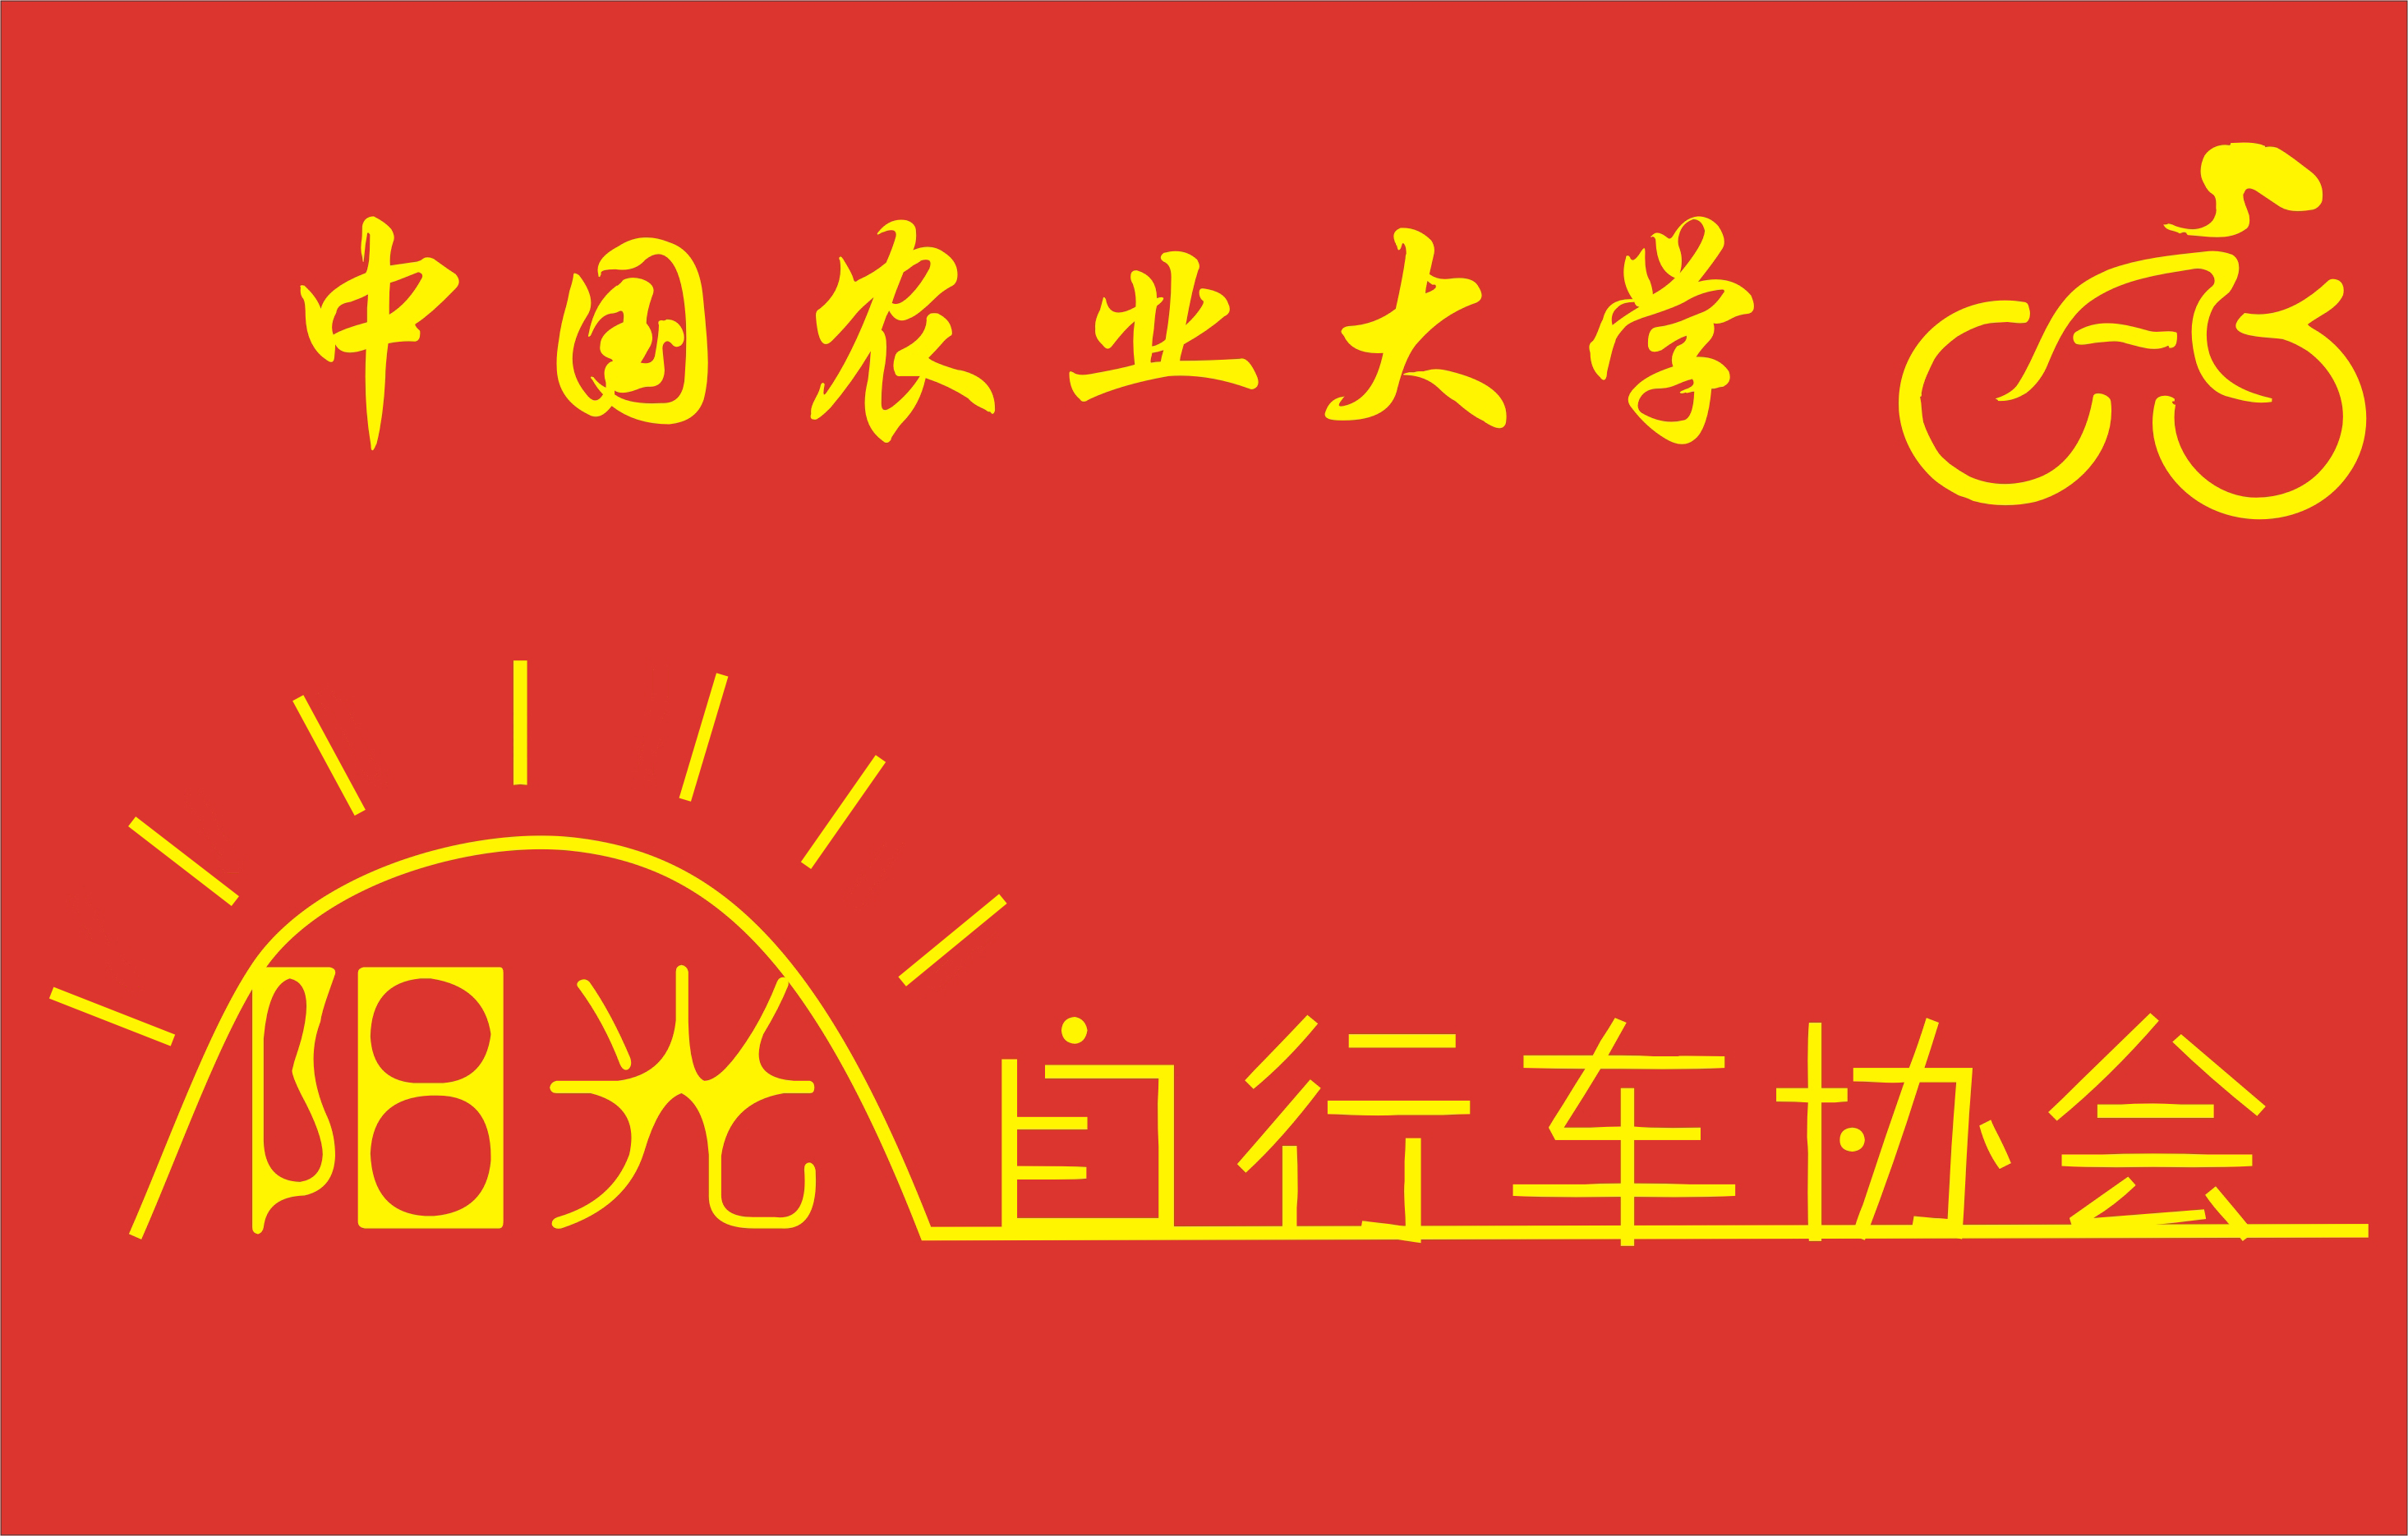
\includegraphics[width=1\linewidth]{fig/会旗.jpg}
\end{figure}

\tableofcontents
\newpage 
\setcounter{page}{1}
%-------------- 设置页眉页脚 -----------------%
\pagestyle{fancy}            
\fancyhf{}                  % 清空原有样式     
\fancyhead[RO,LE]{\zihao{5}\leftmark}
% \fancyhead[RO,LE]{\fangsong \zihao{5} \rightmark}
\fancyhead[LO,RE]{\zihao{5} ~\thepage~}
\lfoot{}
\cfoot{}
\rfoot{}
\setlength{\headheight}{12.7pt} 
\mainmatter
\chapter{日常活动}
\section{晚训}
\label{sec:晚训}

晚训绝不仅仅是一个日常锻炼!!!它更重要的意义是使队员间相互熟悉,增进感情。如果一个队伍的队员们在上路前都没有见过面,路上就很难再把气氛搞起来让大家开心。

晚训时间为每周的一、三、五晚上,具体的晚训时间根据实际情况定;一般来说,集合签到时间安排在 9:00-9:10,晚训结束时间不应超过 10:25(男生送完女生回宿舍后仍有洗澡时间)。当然,如果大家想坐下来聊聊天,就继续聊。
\begin{figure}[htp]
    \centering
    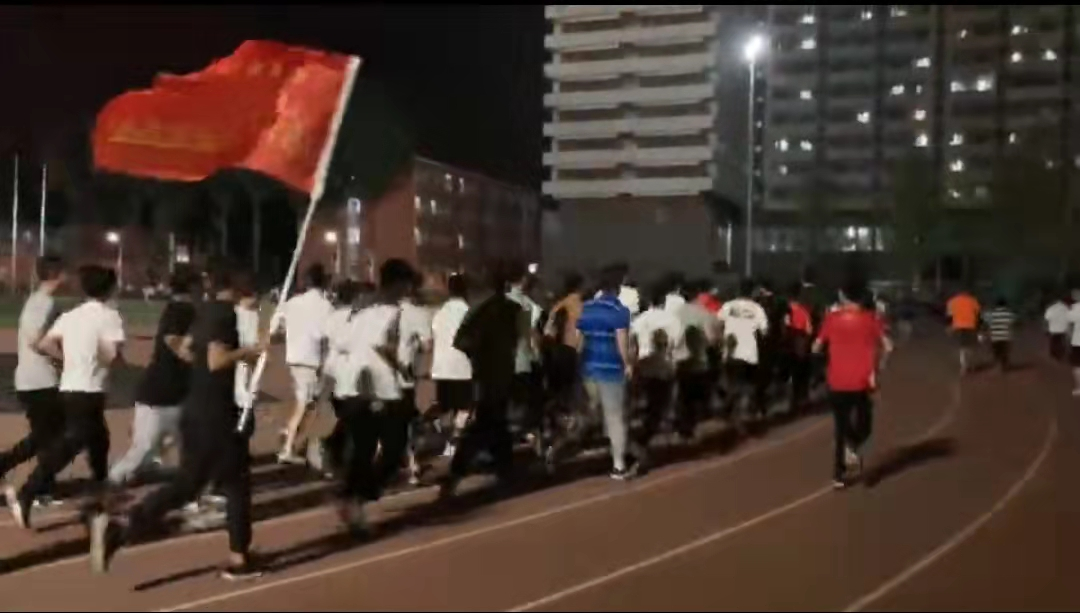
\includegraphics[width=1\linewidth]{fig/晚训}
    \caption{晚训}
\end{figure}

\clearpage
\subsection{通知安排}
晚训当天18:00左右活动部发晚训通知,晚训通知可参考 \pageref{ssec:晚训通知} 页

\subsection{人员安排}
需要有一个晚训队长负责晚训,刚开学由活动部安排执委带晚训,之后为培训新人,酌情给新人带。

\begin{tips}
根据往年经验,应当在学期初就安排好每一天由谁来负责晚训。如果当天被安排的人临时有事,由ta来负责找带晚训的人。这样可以减少很多问题。
\end{tips}

晚训队长要提前准备好旗杆和旗子,提前到晚训场地,并做好签到记录。在晚训期间,带领大家做好各项运动。晚训结束后,进行签退,并将晚训名单发到QQ群和微信群。
\subsection{活动内容}
\begin{itemize}
    \item 晚训前晚训成员在晚训队长处签到。
    \item 在跑步开始前,再次提醒大家签到,并开启闪动校园。
    \item 先热身跑2圈;然后做基本的准备运动:头部运动、肩部运动、扩胸运动、体转运动、振臂运动、弓步压腿、侧压腿、双手握脚踝30秒、手腕脚腕活动;之后继续慢跑:最后一圈为冲刺圈,能跑多快跑多快。
    \item 跑步结束后提醒大家増衣,关闭闪动。
    \item 跑完之后拉伸:围一圈压腰(20次)、拉小腿、拉大腿、俯卧撑\&平板支撑(秋季学期和春季初男生10个俯卧撑或平板支撑1min,女生40秒平板支撑;开始暑期积分之后,先20个俯卧撑,10个一组,然后平板支撑,男1min女50s)、拉肚皮、拉肩、拉背;
\end{itemize}
\subsection{注意事项}
\begin{itemize}
    \item 秋季学期起步5圈,之后大概一个月左右加两圈,寒冬时不再增加;春季学期起步7圈,之后每两周加两圈,直至加到15圈。
    \item 开始暑期积分时,跑步速度要逐渐加快且改为变速跑,每两圈变速\footnote{变速即男女生队伍中位置改变,第一排速度不变,最后一排依次冲到第一排直到男生/女生换位完成。变速跑会进一步消耗跑者的体能,实现更好的训练效果}一次;
    \item 跑步过程中会有口号。偶数圈开始跑时喊口号:车协,加油!加油,车协!(当冲刺跑恰好为偶数圈时,选择不喊口号。)如发现有新生因害羞等原因不好意思喊口号时,应善意提醒。
    \item 当有人掉队时,由队长,或队长安排其他老人陪着该同学跑圈;
    \item 晚训结束之后晚训队长要带大家一起聊天做游戏。刚开始大家普遍不认识时通常为自我介绍,如果觉得自我介绍比较无聊,可以转换成互相介绍身边的同学。夏天天气炎热时会组织一起吃瓜。  
    \item 大家解散时,男生要将女生送回宿舍。
    \item 晚训没有强制完成的要求,但是参加骑行活动往往需要参加过晚训。
    \item 暑期/冬训积分时:迟到\footnote{迟到是指在集中签到后,正式跑(非热身跑)前加入大部队参加晚训。正式跑的时候加入大部队的,不做签到。}需要扣掉一半的分值,
\end{itemize}

\section{周末单日骑行活动}

\subsection{活动前的准备}

\paragraph{活动前一周周六}

活动部部长需选拔一名活动经验较为丰富的老人与一名车协大一新人担任活动队长,并指导他们完成活动策划书,培训队长使其对活动的每一方面做到充分的了解。

策划书内容须包含:队长介绍,路线设计,报名信息和活动信息,设计宣传首语,主要目的地介绍。

时间:周六晚22:00前将word版策划发至执委群。

\paragraph{活动周周一}

宣传部收到策划,于周一中午2点前发出活动报名的微信推送。

队长应当在阳光车协微信群,QQ群进行文字宣传。

宣传过程中队长应当多参加晚训,与队员相互认识相互了解并且进行有效沟通,观察已报名队员的身心状态。

\paragraph{活动周周三}

周三晚 18:00 点报名截止,办公室整理活动名单并检查晚训情况,随后队长通知并安排没参加晚训的队员周四晚补训,未能参加补训者队长有权取消其活动资格。一般周五不得补训。

办公室还需要统计借用车辆并及时联系实践部借车。如果借头盔/车的数量超过了车棚的头盔/车持有量,要及时私聊老人借头盔/车。

\paragraph{活动周周四}

队长安排职务,并把做好的职务表发到执委群里给大家审核。如果大家没有异议的话,办公室把职务安排写到策划里,并把格式转成 PDF\footnote{PDF文件在不同的设备的传输过程中上不容易发生格式错误。} 发到执委群。



队长发布检车短信\footnote{检车短信模板见 \pageref{subsec:检车通知} 页},通知大家检车。在学期前期,不建议把检车地点定在车棚,新人不容易找到车棚。

队长将全体参加活动的队员拉入活动群中。活动群应包括QQ群与微信群,此外,还应把负责收租车费和保险费的办公室主任拉进群中

周四晚向全体参加活动的队员发短信通知周五中午检车。

\paragraph{活动周周五中午}

检车

地点:东区:东区车棚;西区:7 号楼和 8 号楼之间的空地处

流程:签到—办公室负责,每人签到拿取策划。

队长点名签到,手拿策划具体介绍活动,带领大家阅读策划书,提醒大家活动集合时间、地点、距离强度。带读安全协议,提醒所有人认真阅读安全协议并签字,出发前应上交安全协议,否则不予参加活动。

对全体队员进行团队安全培训:
\begin{itemize}
    \item 介绍前骑,后骑,队医,队长,以及他们的职责
    \item 介绍突发情况处理:摔车,掉队
    \item 介绍骑行手势及口号教学。
\end{itemize}

提醒前骑熟悉活动路线;提醒后骑提前准备好后骑包并于活动前一晚到办公室拿后骑包和防潮垫;提醒大旗活动前一晚到办公室拿大旗和旗杆并在活动出发前绑好。

借车:队长通知实践部成员带领所需借车的队员前往车棚取车。

检车:队长安排所有队员跟随实践部成员学习检车、修车并检查自己的车辆。

监督所有队员试骑车辆,队长观察情况,如有一些新人不会骑车应当马上进行教学或劝退活动。

所有活动成员在车辆检查完毕且检车相关流程全部完成后请示队长方可离开。

队长须在活动前一天晚对全体参加活动队员发短信提醒集合时间地点及活动相关事宜。

检车项目可参考:\pageref{sec:检车}页
\paragraph{活动日前一天晚}

提醒各职务尽到自己的职责

\begin{itemize}
    \item 前骑应准备好路书并发在群里,准备好手机支架
    \item 后骑应准备好后骑包
    \item 大旗应准备好旗子和旗杆
    \item 队医应准备好队医包
\end{itemize}

另外提醒所有人参加活动的成员第二天集合时间,提醒大家上好闹钟。
\subsection{活动中}
\subsection{活动结束后}
\paragraph{活动后一两天}
西区办公室主任进入活动群(或者提前进入活动群),收策划费和保险费。
\paragraph{活动周次周周三}

在QQ群中提交队记与视频照片,便于宣传片做推送。队长还应提交队长总结。

将队记和队长总结整理好放到执委QQ群中,便于下一次活动查阅。

\paragraph{活动周次周周日}

提交本次活动的检讨至活动QQ群和微信群。
\subsection{注意事项}
    \begin{itemize}
        \item 如果活动安排在周五,那么办公室一定要尽快买保险,不要拖到周五再买。因为保险只能买第二天的,不能买当天的。
        \item 如果连续两天安排了两次活动,两次活动队长要做好租车,租头盔,准备后骑包和队医包的工作交接。
        \item 如果活动出发时间较早,车棚有可能还没有开门,这就意味着需要提前跟车棚老板说,让他早点来开门。
        \item 同样的,如果活动回来的晚,要提前想好把车放到哪。
    \end{itemize}


\section{多日骑游活动}

单日活动中提到的事宜,多日活动同样需要注意,下面说说跟单日活动不一样的。

\subsection{活动前}

根据以往队长的经验和总结,提前获取每天的食宿安排信息,可能需要提前预定,联系店主。

根据实际情况做足够准备,包括物资上(夜骑需要准备前灯和尾灯,生活用品等)

\subsection{活动中}

每天中午,晚上安排发前站,提前找食宿点

每天晚上开例会,总结当天骑行情况,并说明第二天行程安排,安排第二天职务(前骑,后骑,大旗,队医,队记),前骑一般不连续安排,第二天及以后的职务安排可以更多考虑个人意愿,让更多新人尝试。

晚上组织后骑帮大家检车,补好当天的破胎,确保出发不受阻。后骑还应当在当天晚上检查一下所有人的轮胎是否有气,防止出现慢撒气没有发现的情况。

前骑需要在早上出发前为大家找好早餐点,并在大家集合后带领大家就餐。

凡是集合出发均须确保所有队员到齐,必要时点名,早上离开宾馆组织后骑查房,防止遗漏物品,集合时间须通知到位。

活动中一些其他的重要事情的决策和小事情决策均由队长下发。

活动过程中所有人不得单独离队行动,女生离队活动须有男生陪同。较远活动须向队长说明,有任何情况及时联系队长。(要求队员均存下队长手机号码)

遇突发情况若较为严重,及时选择就近医治或考虑送返。

运车和搭车问题:(如十一秦皇岛)提前一天联系物流货车托运自行车,并联系大巴车(可向当地老板了解情况)

若有个别队员因特殊情况须离队,根据实际情况合理安排运车和搭车,队长需要留在队伍当中。

\subsection{活动后}

多日活动总体情况,将出现的问题集中,对队员的表现变化情况做总结,给予表扬或批评。

将多日活动所有队记和摄影资料整理在一块。

提醒财务做出最后明细账单,队费多退少补。


\section{校内拉练}
校内拉练实属被迫无奈,如果有可能的话,尽量选择校外骑车拉练。很多东西,不进山不爬坡是感受不到的,希望校内拉练也可以让大家热络起来。虽然是无奈之举,但负责人和执委的认真筹划也可以让队员们感受到车协的快乐氛围。

\subsection{校内定向越野}
定向地点推荐西校区,西校区对大部分人都比较陌生,不会太枯燥。

活动负责人在学校内定点,在每个定位点设置一定的关卡,如特定姿势拍照打卡;队医知识、长途骑行经验问答;补胎、调蹭碟、装手机支架、调座管高度等常见简单问题的解决。按报名人数均匀分队。提前通知校车时间,避免迟到。活动结束后可安排西区约饭。

负责人定向开始前,收走除小队长以外所有人的手机,一队一张地图,各队按完成时间排名次,名次靠前有奖励。
\subsection{校内长跑}
其实就是一个加长版的晚训,比平常晚训多跑几圈,大概跑个20圈的样子,可以跑的慢一点。在热身环节可以带大家做一些小游戏,在跑完步之后,可以搞点桌游让大家玩一玩,也挺有意思的。
\subsection{讲座}
% \section{特殊活动}
% \subsection{露营}
% \subsection{夜爬百望山}
% \subsection{东西区对跑}
\section{室内活动}
\subsection{概述}
\subsubsection{活动预热}
和骑行活动一样,也应当提前发推送,在q群和微信群提前宣传,在晚训结束后宣传。

比较重要的活动如新生见面会,暑期宣讲会,可给新人发短信邀请。

\subsubsection{人员准备}
人员安排包括找活动负责人(策划人)和活动主持人。其中活动负责人需要提前编写策划,安排活动流程与任务分工;活动主持人负责制作PPT,准备主持词,主持整个活动。
\subsubsection{物资准备}
\begin{itemize}
    \item 考虑是否有抽奖环节,如果有,应当提前准备奖券和奖品。
    \item 准备小零食\footnote{打开拼多多,在多多买菜里买零食会非常便宜},周边产品(明信片,徽章),手环
    \item 会旗\footnote{要考虑好会旗的摆放位置,是否需要准备胶带等其他辅助摆放会旗的物资。}
\end{itemize}
\subsubsection{场地准备}
考虑到社工部的工作延迟,建议提前一周借教室。借教室的细节见 \pageref{sec:借教室}。

安排几个人提前来布置场地:摆放零食和周边,摆放会旗,直播设备。

最重要的是还要检查多媒体功能:声音大小,视频和音频播放、投屏、PPT播放和话筒声音大小。

在活动开始前20分钟左右,可以播放B站视频来预热活动。

\subsubsection{活动后}
应当安排两到三个执委进行最后的收尾工作,把教室里的垃圾清理干净,检查桌洞中有无落下的的个人物品,擦干净黑板。
\subsection{新生见面会}
新生见面会一般定于百团大战当天晚上。

参考时间为:19:00-20:15

新生见面会大约到场80人左右,除去老人,理事,执委,新人到场大概4,50人。

负责人分成两个方向,一个是主持人,一个是策划人。

负责人最好能在活动前一周就能完成好策划,前三天完成好PPT,以待有充分的时间进行协调和更正。

负责人不要把所有的活都览在自己身上,要学会充分调动其他执委部门。主持人可以找外联部,宣传部;活动的物资,奖品安排给办公室;见面会的游戏可以找实践部做裁判;教室的预约可以找会长,理事;场地的布置可以发动大部分执委。

负责人才策划中用到的人最好能够逐个通知到位,比如需要上台的要叮嘱准备好发言内容;需要干活的指出需要干什么。

游戏状况良好,新人参与比较积极,没有出现尬场,冷场的情况。推人争霸赛和画画接龙效果不错,台下有比较好的反应。吸纸片因为场地原因,只能一组进行展示,稍微缺少竞技性。





\begin{figure*}[!htb]
    \centering
      \subfigure{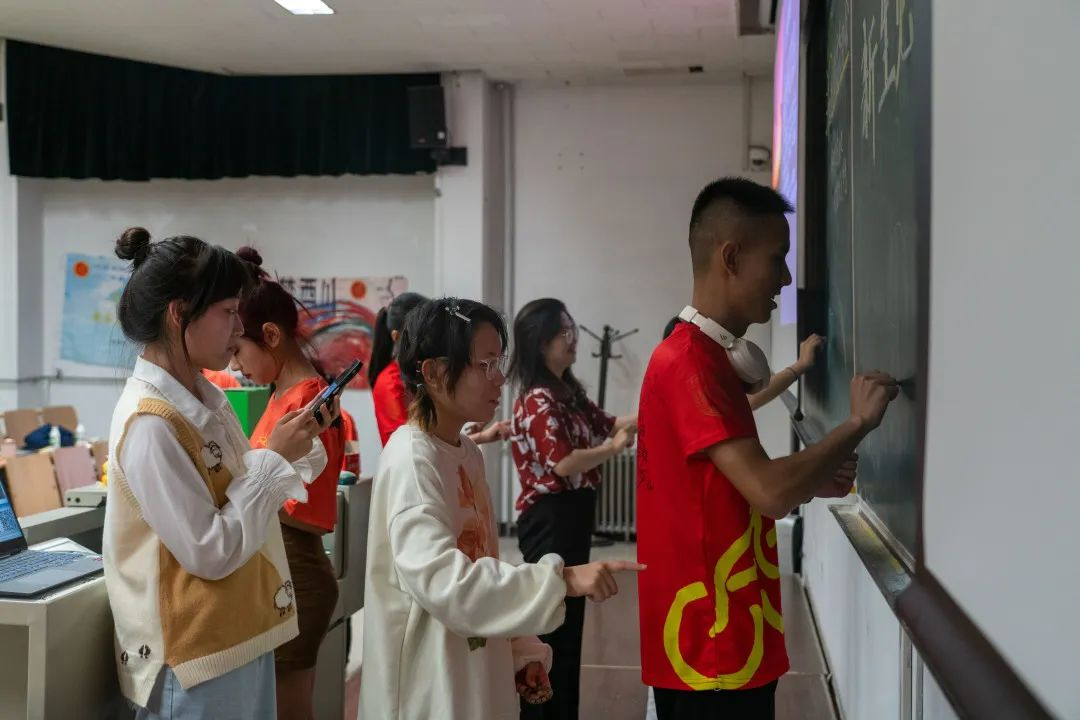
\includegraphics[width=0.45\textwidth]{fig/新生见面会1}} \quad 
      \subfigure{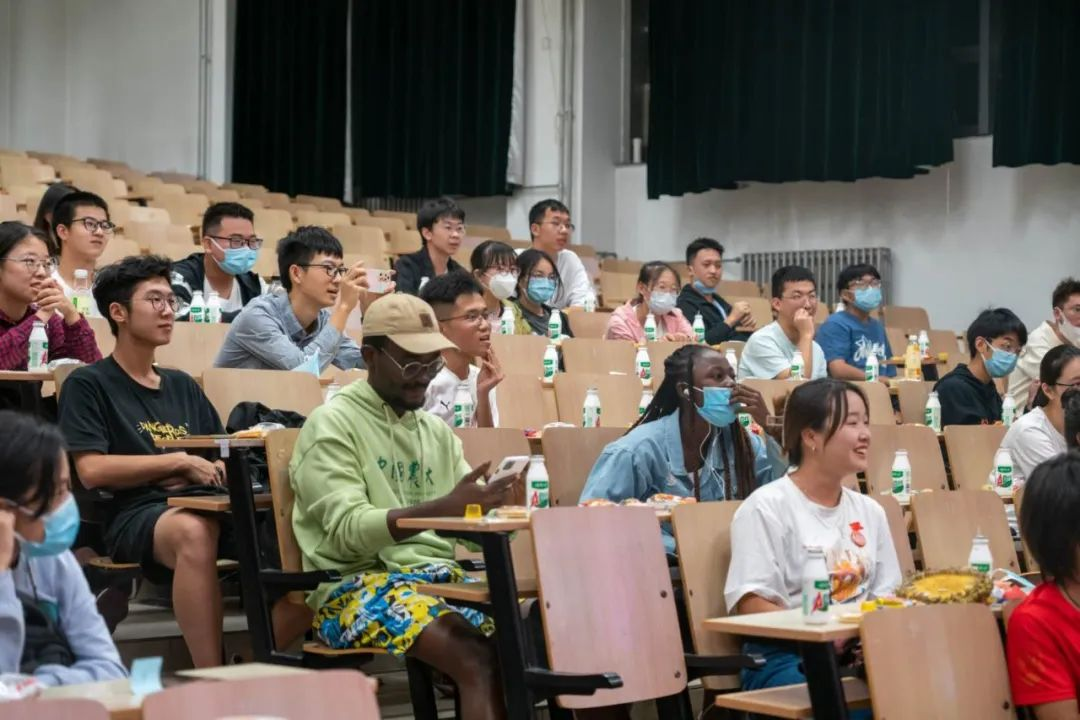
\includegraphics[width=0.45\textwidth]{fig/新生见面会2}} 
        \caption{拍于20229月25日}
  \end{figure*}


\subsection{暑期报告会}

执委会长带领执委会讨论,并由理事会最终确定负责人。

    举办时间在10月。

    负责人需在活动前一个月完成书面策划书并提交理事会审核。

    负责人须在筹备活动前翻阅车协历届办会资料,学习办会方法,努力探索积极创新提高活动质量。

\subsection{冬训宣讲会}


\subsection{暑期宣讲会}
\begin{figure}[H]
    \centering
    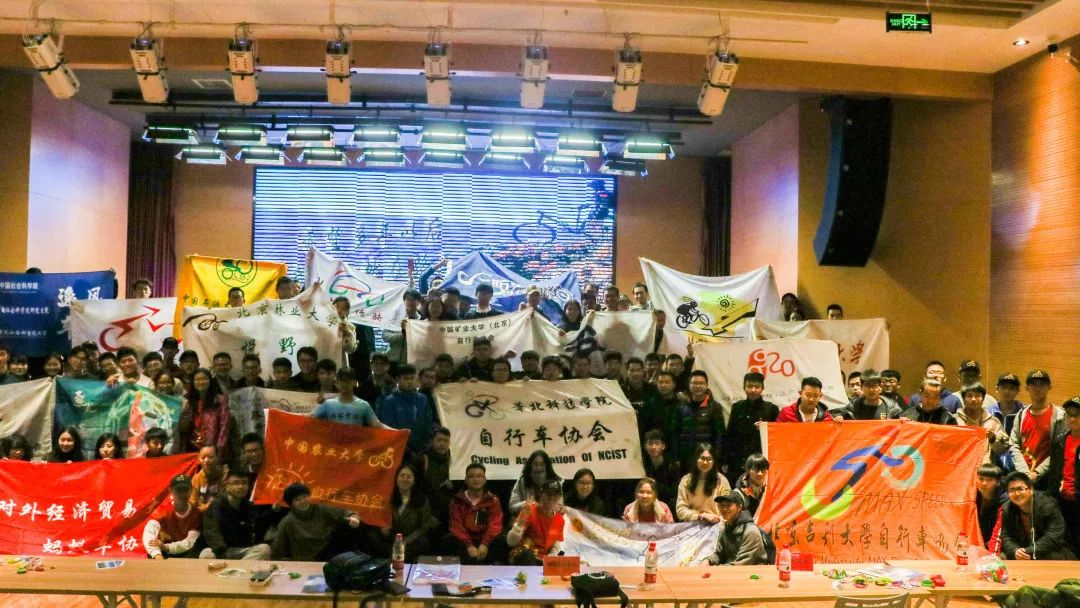
\includegraphics[width=0.7\linewidth]{fig/暑期报告会.jpg}
    \caption{摄于2018年11月10日}
    \label{fig:}
\end{figure}
   由理事长带领理事会讨论,并由理事长和执委会长作为负责人。

   理事长须与理事会讨论并制定暑期远征拉练选拔方案,并在大会上进行宣讲。

   暑期队长需要制作自己路线的ppt并在台上宣讲。
\subsection{换届大会}
\begin{figure}[H]
    \centering
    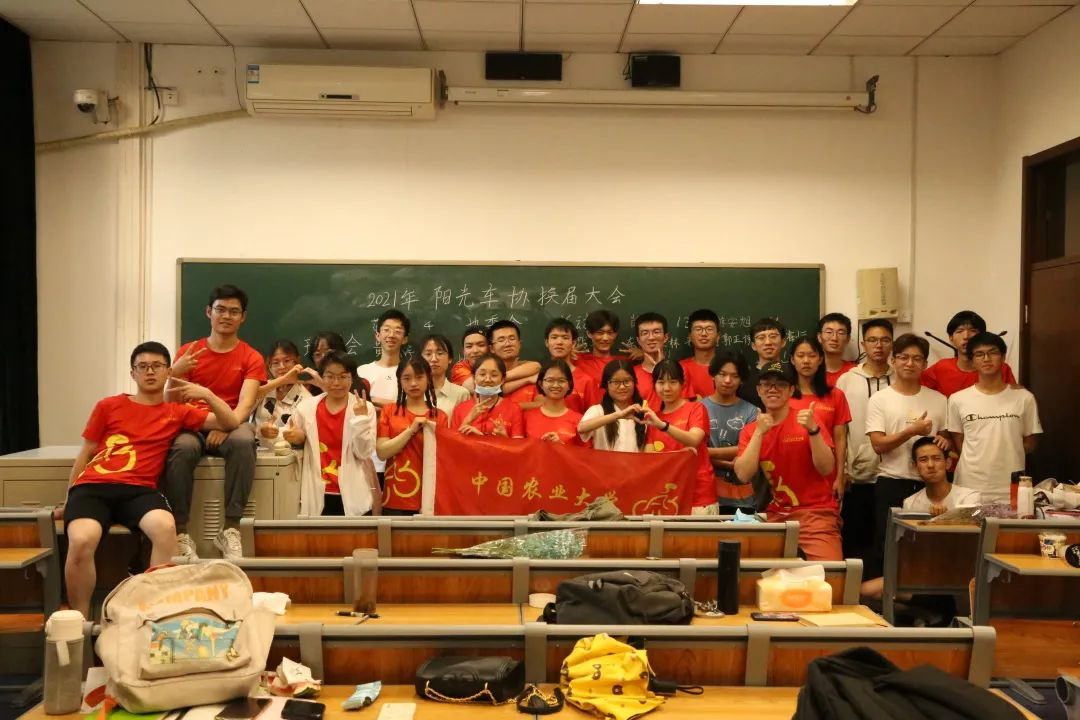
\includegraphics[width=0.7\linewidth]{fig/换届大会.jpg}
    \caption{摄于2021年6月20日}
    \label{fig:}
\end{figure}
\subsection{生日会}
生日蛋糕参考标准:20寸,388元

\subsection{冬训宣讲会}

\section{技能培训}
\subsection{队医培训}
\subsection{队长培训}

\section{学校主题活动}
\subsection{秋季百团大战}
物资准备:零食,车协会旗,暑期队旗,明信片,周边(徽章,手环)
\begin{figure}[H]
    \centering
    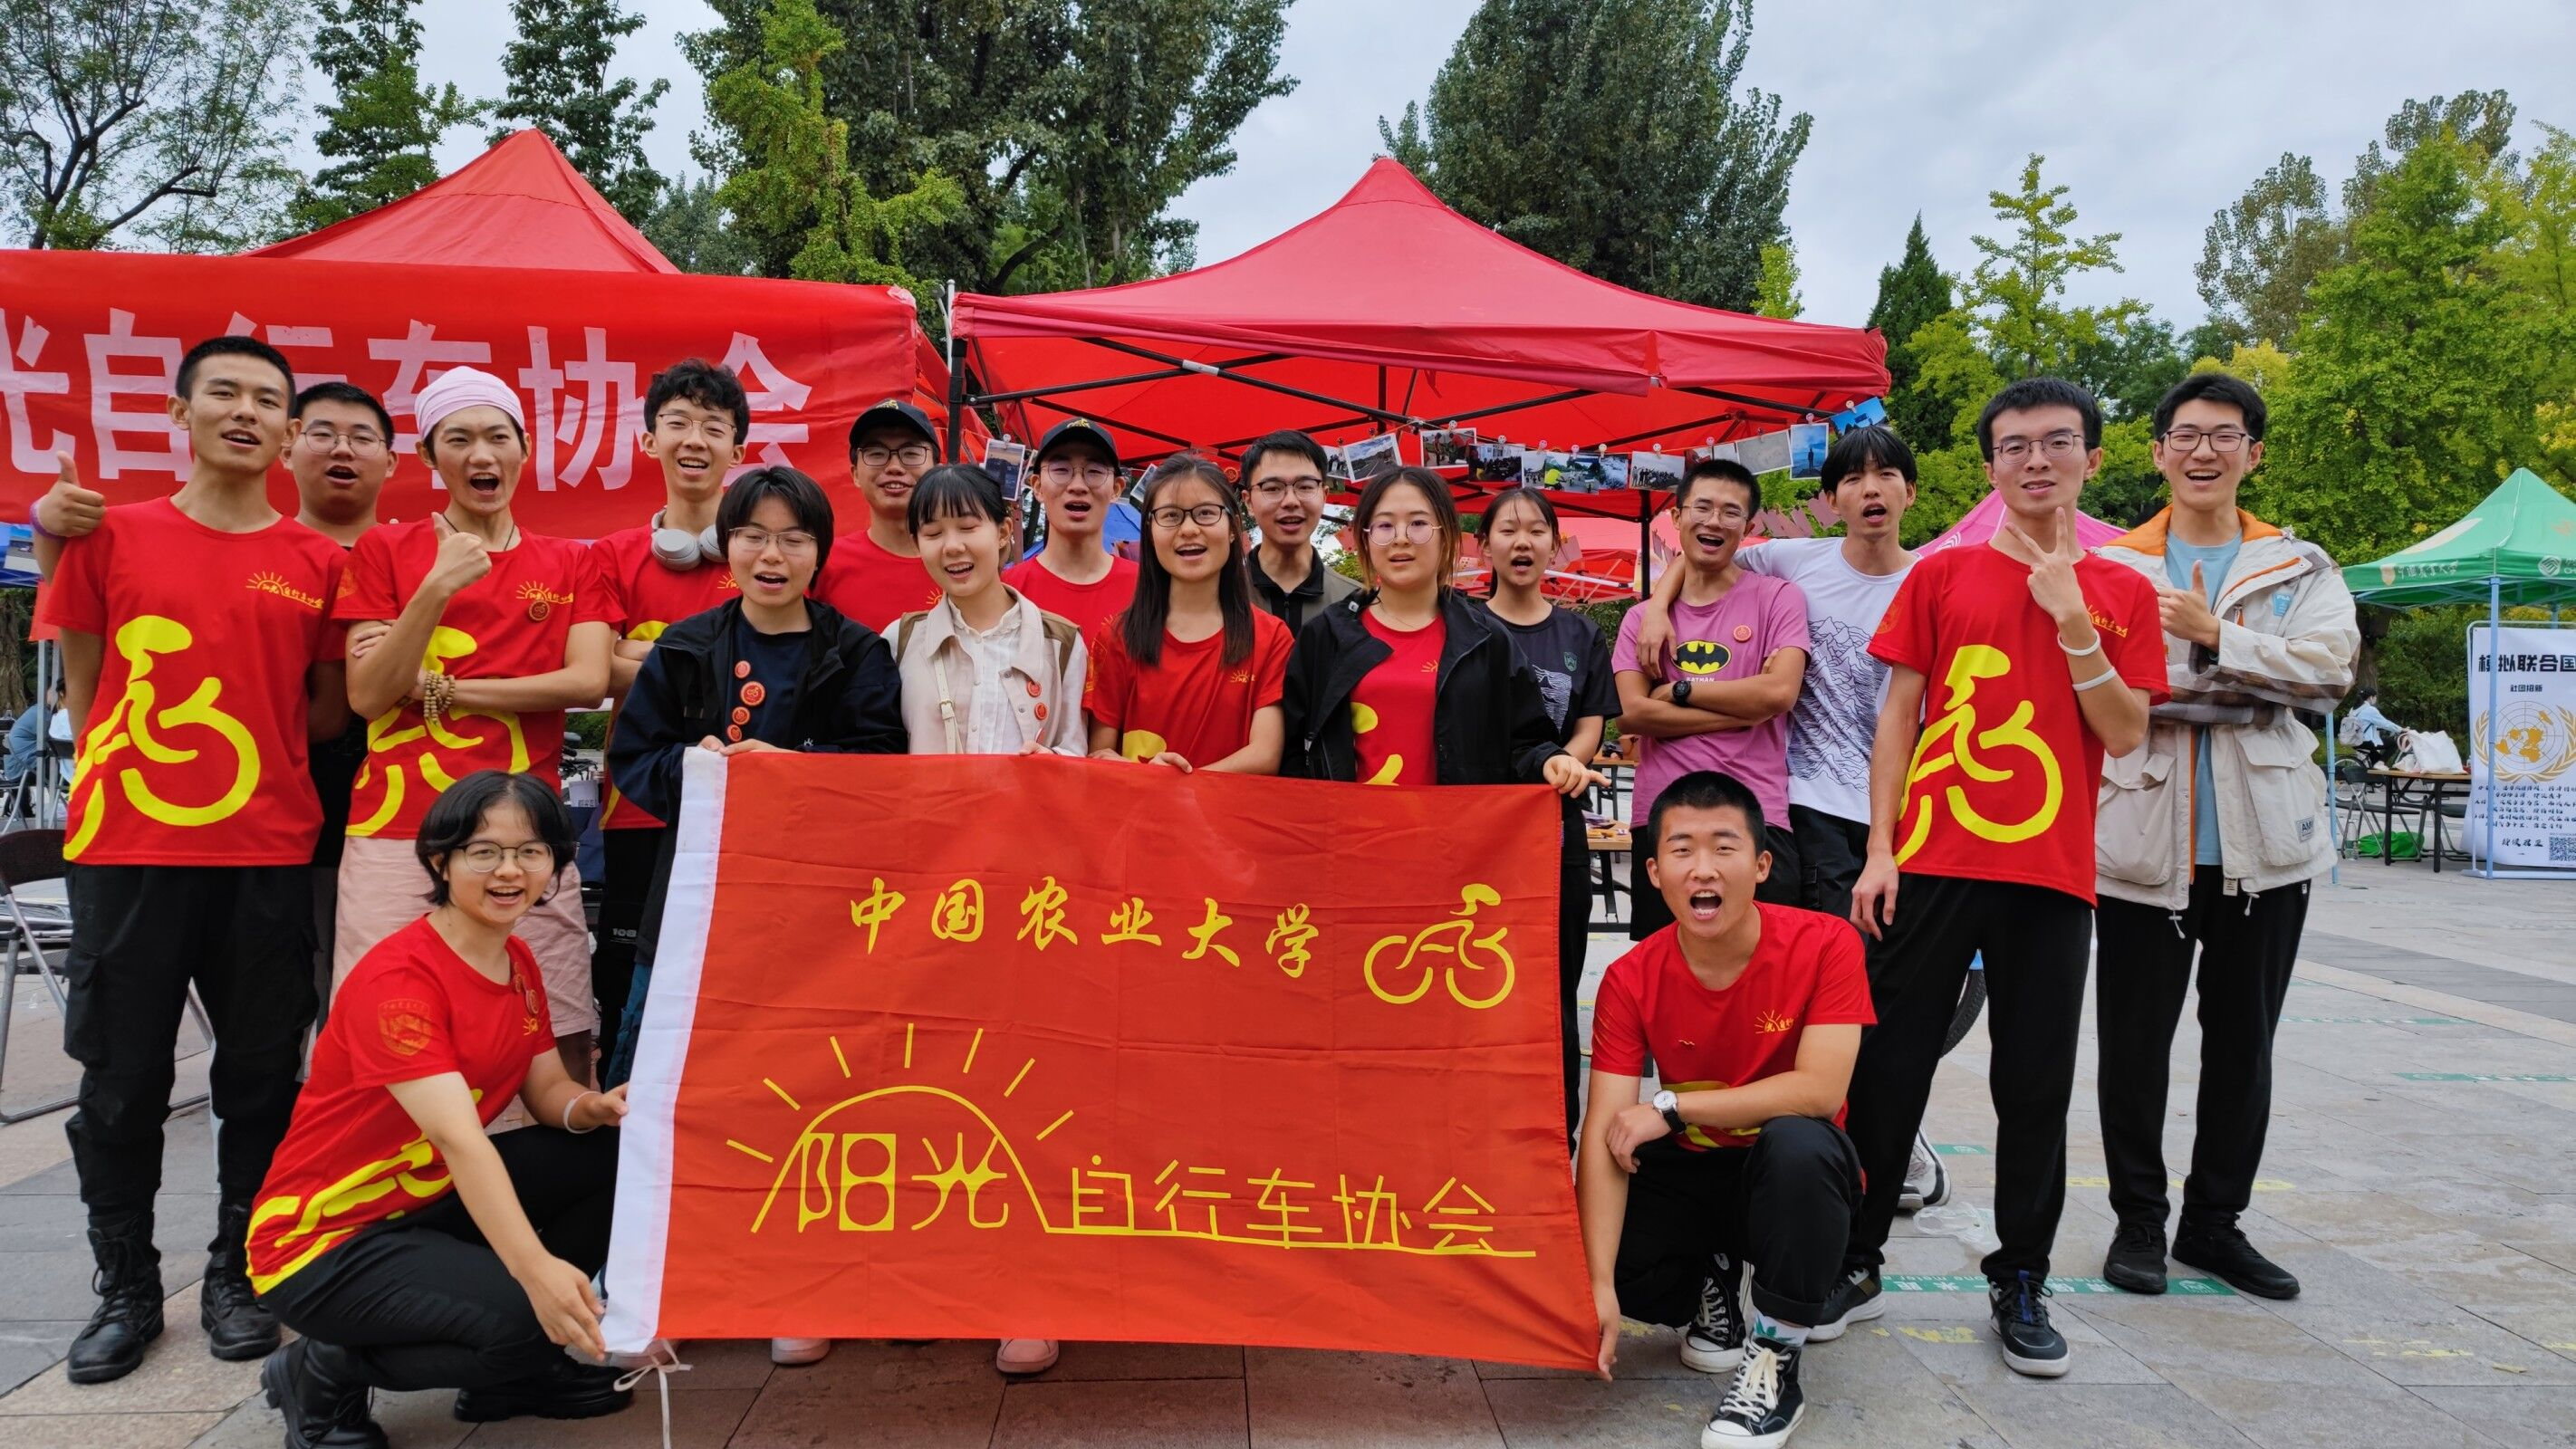
\includegraphics[width=0.7\linewidth]{fig/百团大战}
    \caption{摄于2021年9月25日}
    \label{fig:百团大战}
\end{figure}

\subsection{金色的希望}
\begin{figure}[htp]
    \centering
    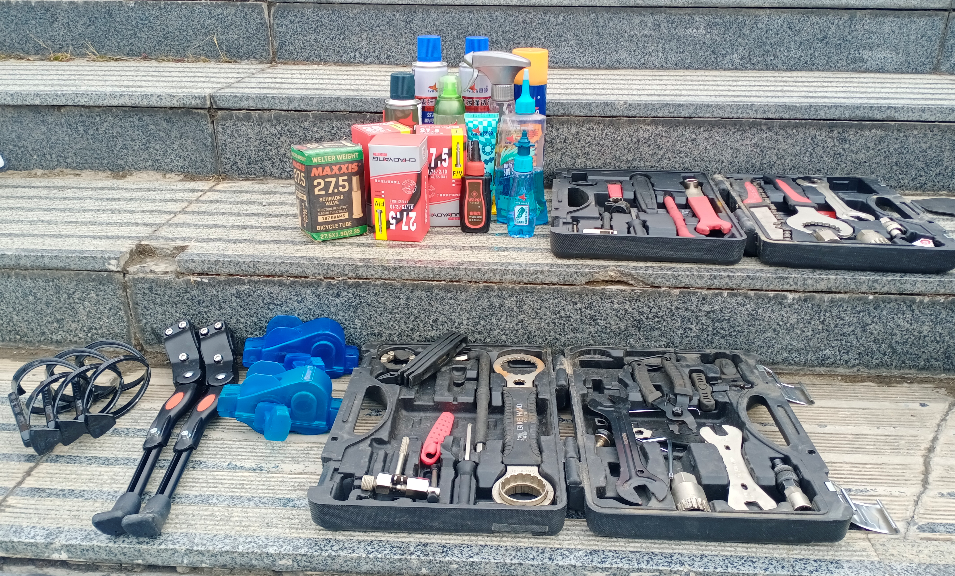
\includegraphics[width=0.7\linewidth]{fig/金色的希望}
    \caption{摄于2020年12月2日}
    \label{fig:}
\end{figure}

此活动是车协稳定的物资来源。一般来讲,我们的特色活动为:义务修车。此活动可以报销一批活动经费,一般会购买以下物资:

自行车保养用品:链条清洗剂,除锈剂等。

自行车车身装备:水壶架,副把等。

自行车维修工具:组合,工具箱等。

总计预算控制在2300左右即可。
% \subsection{校庆嘉年华}
% \subsection{春季百团大战}
% \subsection{五四嘉年华}
\subsection{五月的花海}
在之前的几次五月的花海中,我们主办的活动主要是运动打卡。即上传运动记录截图打卡,最后依照运动强度来评奖。此外,还有一个创意赛道,上传跑步(骑车)的轨迹,后面让大家投票选出最有创意的路线,给予奖品。

\begin{figure}[H]
    \centering
    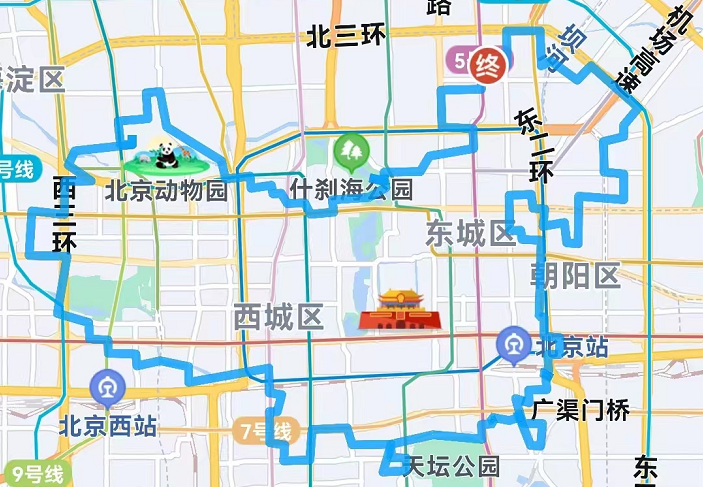
\includegraphics[width=0.7\linewidth]{fig/地图路线.png}
    \caption{于2022年10月1日完成,路书编号:3401283}
    \label{fig:百团大战}
\end{figure}

\section{检车}
\label{sec:检车}
本章中提到的检车是指广义上的检车,即包括了检车本身在内以及宣读安全协议等其他检车时要做的事项。
\begin{itemize}

\item 刹车灵敏度

\item 快拆

\item 变速

\item 前叉

\item 绑绳

\item 座椅高度

坐在坐垫上,用脚后把脚踏踩到最低点,腿蹬直。这个位置的坐垫就可以。过程中找个人帮忙扶着车子。

或站在车子旁边,坐垫的高度在腰部靠下的位置,不过没上面那种准。

正确的坐垫高度坐在坐垫脚是碰不得地的。

\item 蹭碟

\item 行李的捆绑

绑绳必须收紧并勾稳,前后左右对称,不得有任何绳或带裸露在外,避免卷进轮胎发生危险。
\end{itemize}
\section{体测}

\subsection{跑步体测}
跑步体测前要有负责人带着大家做热身,就和平时晚训热身一样,慢跑两圈+压腿等。热身既可以减少大家运动受伤的可能,也能增强大家的运动表现。

志愿者的职责包括:递水,递毛巾,驱赶跑道内圈干扰体测的人员,记录每个人的成绩。

和骑车跑步一样,志愿者也需要准备物资。凉水,热水,简单的补充能量的食品,中暑药物等。

\subsubsection{秦皇岛体测参考标准}

男生4000米 女生2800米

男生30分钟内(7.5min/km) 女生25分钟以内(8.9min/km)
\subsubsection{冬训体测参考标准}
不做跑步要求。
\paragraph{暑期体测参考标准}
男生:6000米(15圈),要求30分钟以内完成;(5min/km)

女生:4800米(12圈),要求28分钟以内完成。(5min50s/km)


\subsection{骑车体测}

体测要安排体测负责人。

负责人要招募体测志愿者,买物资。

物资包括:开水,纸杯,水果(西瓜,香蕉),饮料。

一般会租一辆燃油车来便于携带物资。

\subsubsection{秦皇岛体测}
不做骑车要求。
\subsubsection{冬训体测}
蟒山9公里爬坡:

男生60min、女生70min
\subsubsection{暑期体测}
选取妙峰山经典爬坡路段作为体测路段,全程约21km,累计爬升约900m。全体队员均由妙峰山山脚牌坊处出发

骑行队:

终点位于妙峰山山顶停车场(21km)

男生90分钟内完成,女生105分钟内完成

实践队和短途团:

男生终点位于妙峰山山顶停车场(21km),要求95分钟内完成;女生终点位于妙峰山山腰水站(14km),要求65分钟内完成
\subsection{给体测人的一段话}
跑马拉松的时候,你的身体和脑袋都要你停下来,你的身体不想要继续跑,但你还是使尽全力踏出每一步

马拉松的最后,最后一小段路是最难熬的,因为身体已经跑了好几公里,被推到极限,一公里接着一公里,潜意识里一直想要停下来,但是脑袋里另一个声音说不行,身体和心灵不断地对抗。

我们算出生理上的数据,也算出风的阻力,空气的阻力,鞋子的能力,这些都算得出来,但还有一块空白,无法解答的地方,该如何量化心理素质,要如何量化一个人超越极限的决心,做到科学上认为不可能的事情。

\href{https://www.bilibili.com/video/BV1pb411K74L}{挑战马拉松破2纪录片-breking2}
\subsection{体测排名计算方法}
如果只有一个项目(比如只有爬坡),显然我们可以按照用时多少直接进行排名。但如果有两个项目,那么我们必须要有一个算法来结合排名。

首先,要将单项用时转化成单项得分,然后再把单项得分乘上权重,得到最终得分。

参考计算方式如下:

符号说明:

\begin{itemize}
    \item 综合成绩 (百分制):  $S$ 
    \item 此人跑步成绩 (单位: 秒):  $S_{1}$ 
    \item 此人骑车成绩 (单位: 秒):  $S_{2}$ 
    \item 在同性中, 最长跑步用时:  $\max _{S_{1}}$ 
    \item 在同性中, 最短跑步用时:  $\min _{S_{1}}$ 
    \item 在同性中, 最长骑车用时:  $\max _{S_{2}}$ 
    \item 在同性中, 最短骑车用时:  $\min _{S_{2}}$ 
    \item 跑步得分权重:$\alpha$
    \item 骑车得分权重:$\beta$
\end{itemize}

\[S=\left(\alpha \times \frac{\max _{S_{1}}-S_{1}}{\max _{S_{1}}-\min _{S_{1}}}+\beta\times \frac{\max _{S_{2}}-S_{2}}{\max _{S_{2}}-\min _{S_{2}}}\right) \times 40+60\]

例: 小A(男)的跑步用时为  $1609 \mathrm{~s}$ , 骑车用时为  4$187 \mathrm{~s}$ ; 男生最长跑步用时 为  $1772 \mathrm{~s}$ , 最短跑步用时为  $1531 \mathrm{~s}$ ; 男生最长骑车用时为  $5438 \mathrm{~s}$ , 最短骑车用 时为  $4170 \mathrm{~s}$ .权重均为 $0.5$ 所以小A的综合得分为

\[S=\left(0.5 \times \frac{1772-1609}{1772-1531}+0.5 \times \frac{5438-4187}{5438-4170}\right) \times 40+60=93.26\]

注:在此方法中,最终得到的得分会落到 $[60,100]$ 中

\section{其他活动}
\subsection{刷楼}
一般在百团前一到两周。

海报大约需要六百张。

\subsection{包饺子}
车协会在冬至那天包饺子。

前期准备:找一个提供包饺子服务的食堂,2021年冬至联系的公二食堂,场地是公二的灿灿学堂。根据报名人数定饺子皮和饺子馅的数量。一斤皮对应一斤馅可以包出四十多个饺子。除此之外准备桌游和零食饮料,辣椒和醋食堂都有,搞点腊八蒜什么的就行。

活动流程:吃喝唠嗑。包饺子煮饺子吃饺子,唠嗑,桌游......

活动预算:2021年收费是26/人
\begin{table}[H]
    \centering
    \begin{tabular}{|c|c|c|c|c|}
    \hline
    ~  & 素馅 & 猪肉馅 & 牛肉馅 & 饺子皮 \\ \hline
    单价/斤 & 30 & 40  & 50  & 3   \\ \hline
    \end{tabular}
\end{table}

\subsection{包粽子}

\chapter{骑行技巧}
\section{放坡}
\subsection{放坡前的准备}
\begin{itemize}
    \item 放坡前务必检查头盔是否戴稳,手套戴稳。
    \item 再次检车,刹车灵敏度须合适,前叉须解锁,快拆杆须扣紧,仔细检查是否有松动物品,例如手电筒,手机支架,绑带,水杯等等。
    \item 除非天气实在是好到不行,不然都建议大家把爬坡时脱掉的衣服赶紧穿上,放坡时候的风实在是太大了,很容易导致感冒。
    \item 将座椅高度适当调低,最低到双脚能着地高度,以降低重心提高稳定性
\end{itemize}
\subsection{放坡中的注意事项}

\begin{itemize}
    \item 将车挡位调大(起步前调)
    \item 仅允许一列骑行,禁止任何队员超车,超速
    \item 注意避让路面上任意小石子,玻璃,树枝等障碍物
    \item 身体尽量往坐垫后部移动,将重心后移,手臂撑住车把
    \item 注意与右侧路沿和护栏保持距离,注意远离路中黄线(一般保持在路中黄线和路边白线间右半部分)
    \item 双手握紧车把,严禁手离车把或手搭车把
    \item 全程禁止急刹,如果刹车技能掌握较差,不要使用前刹。
    \item 入弯前100m开始减速,入弯后尽量放松刹车防止打滑,自然通过而不超速为最佳
    \item 大型弯道时,入弯前弯道内侧腿抬起,外侧腿伸直,(止脚踏蹭地,并可以稳定重心)车身向弯道内侧自然倾斜
    \item 转弯时,车把务必保持平稳,禁止晃动摇摆或突然转动
    \item 放坡时保持注意力集中,头脑清醒,若实在犯困或有其他情况,缓慢减速并提醒后方,选择稍平直视野开阔处靠右停车,待情况恢复后方可继续前行。
    \item 遇后方来车要提醒前方靠右,前方对侧来车提醒后方靠右,前方右侧有障碍物需提醒后方减速靠左。
    \item 遇突发情况,及时减速避让 ,并提醒后方,不得做多余停留   
    \item 中途发生事故,尽量往路边移动,并在事故点后方100m以外设置路障或者安排专人提醒后方来车,防止二次事故。
    \item 意外摔车时,尽量用手保护关键部位,做防卫动作,尽量控制摔车姿势,如弯道处宁可使车倾斜摔倒也不可翻车。尽量远离有悬崖一侧。侧滑时,可让身体自然翻滚几圈以分散冲击能量。
    \item 与前车的距离要比平路骑行时更大。
    \item 遭遇横风时,保持冷静,扶好车把,缓慢减速。
    \item 请勿牺牲个人勇气强行跟随前车速度放坡,即使与前车渐行渐远,不敢放,或觉得速度过快要量力而行。
\end{itemize}
\section{爬坡}
\begin{itemize}
    \item 拉练、体测不推车。

    \item 为提高爬坡速度,可锁死前叉,调高座椅高度
    
    \item 挡位须合适,踏频不得太快或太慢(建议1.5r/s)

    \item 禁止接近路中黄线

    \item 若因体力爬不动,导致车辆不稳,及时停车休息,勿硬撑
\end{itemize}
\section{过弯}
\begin{itemize}
\item 入弯提前减速。
\item 放松:肩膀放松,双手自然握住车把,一两个手指虚握刹车。
\item 视线:时时注意前方路况,紧盯弯道末端。 
\item 路线:选择路线如下图。
       \begin{figure}[H]
            \begin{center}
            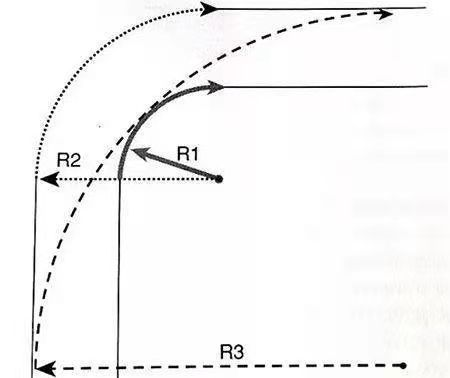
\includegraphics[width=0.6\textwidth]{fig/过弯}
            \end{center}
        \end{figure}
\item 动作:在过弯时,你应该让车身内方向倾斜,身体重心保持在轮胎中轴线上。身子和车子不能一起往弯内倾斜,髋关节往弯外方向偏移,使你的外弯脚承受更多的力,这样能让你在过弯时更好地保持平衡,也能防止摔车时脚被压在车下。内侧脚踏应该在最高点,尽量远离地面,外侧脚踏则在最低点,并将大部分体重压在外侧脚上。将内侧膝盖略向外展可以获得更大的稳定性。

可参考的过弯教学视频 

\href{https://www.bilibili.com/video/BV1xD4y1U7Qh}{bv号:1xD4y1U7Qh}
\end{itemize}

\section{雨骑}
轴承在滚动过程中更易进水,雨骑之后不要偷懒,抓紧抢救一下吧,日积月累总会暴露问题的。
\begin{itemize}
\item 清洗泥沙:车架上有泥沙,最好使用慢速流水的方式将泥沙冲走,不建议用高压水柱冲洗,很可能水会将泥沙冲进五通、轮组花鼓内部。
\item 车架倒立,控出水分:反转车身,将倒出内部积水;擦拭刹车、变速线;将座管取出擦拭干净,也涂上适量润滑油。往往最脏的部位是下叉位置。 
\item 擦干:用抹布擦干。由于车身有烤漆,大部分的油污都可用抹布擦除,擦不掉的可以用去渍清洁剂。铝轮圈以酒精擦拭,不可抹油,以免刹车失灵。
\item 上油:省去上油,链条很快就会锈掉。不宜过多,否则吸附污渍。上完用干净的布擦掉多余的链条油。
\item 在雨骑后要尽快换下湿衣服,防止受凉抽筋。
\end{itemize}

一般车协会提供有偿一次性雨衣。

雨衣售卖小技巧:假如是3元一件购入的雨衣,在活动前可以以3元一件的价格卖给小阳光,在活动中如果还想买的话(往往这时候一件下雨了)以5元一件的价格卖出。
\section{夜骑}
暑期、秦皇岛、五一、难度较大的拉练都可能夜骑,我们会尽量避免夜骑,但我们也从来不会惧怕夜骑。

建议自备手电筒,车协常驻人口往往人手一个,尾灯选带,队伍末尾的人一定要有。

适当拉开车距,扶好车把,集中精神,口号喊得更加积极,也可以更详细,比如白天的''小心``可以变成''小心石头``,我们可以轻松战胜夜骑。


\section{摇车}
什么时候摇车
\begin{itemize}
\item 起步:任何情况下的起步,都可以摇车。很多时候比如十字路口的停车后起步,人多车杂。站立摇车既可快速拉动车的速度也可随机停车。
\item 平路:长距离的骑行,放松是非常关键的。哪怕摇车能维持的时间很短,也该偶尔站起来摇一会车,让上身活动活动,让腿部的肌肉换个方式去发力。短短的十来秒,对于维持接下来的高强度或长时间骑行都有好处。长时间的用一个姿势骑行(特别是快速骑行时)乳酸不容易消解,肌肉一直处于紧张状态。
\item 缓上坡:缓上坡可以用来练习摇车,选择小的齿比,距离较长一点的缓上坡(至少2公里以上的吧),60~70的踏频(随着肌力增强踏频逐步加快)。摇车200米以上才有作用。
\item 短陡坡:选择大的齿比,距离300~500米,60~70的踏频(随着肌力增强踏频逐步加快),一摇到顶。
\item 冲刺:大齿比,距离300~500米(无氧能力也就这么远),踏频有多快就多快。冲刺摇车存在危险。
\end{itemize}
如何摇车
\begin{itemize}
\item 要诀:车摇人不摇,踏随车把动。
\item 车摇人不摇:很多人在初期摇车时大臂、肩部随之一起动,这不光要耗费大量体能还造成用力不集中。练习摇车先掌握要领再慢慢提高踏频。
\item 齿比与踏频:冲刺时摇车齿比较大,长上坡需要小齿比。摇车的时候,大约需要比正常坐踩增加1-2档齿比。因为摇车相对坐踩,作用力增加,如果保持原来的小齿比,会有踩空的感觉。一般摇车的踏频在60-70(即1秒踩1圈)之间比较合适。
\end{itemize}
\begin{figure}[ht]
\centering
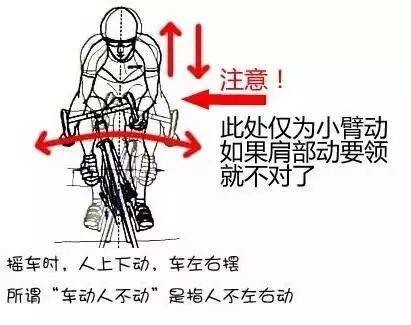
\includegraphics[width=7cm]{fig/摇车1}
\hspace{10pt}  %2张图片的水平距离
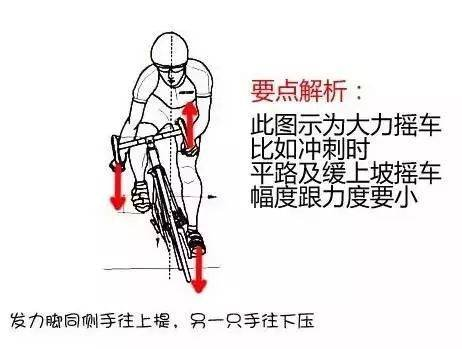
\includegraphics[width=7cm]{fig/摇车2}
\end{figure}

\begin{figure}[ht]
\centering
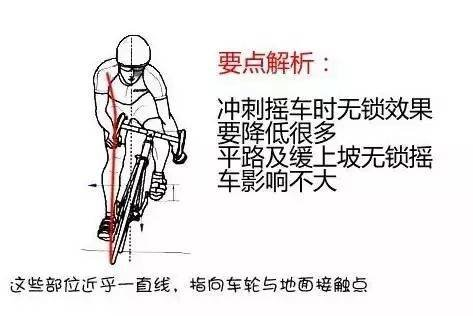
\includegraphics[width=7cm]{fig/摇车3}
\hspace{10pt}  %2张图片的水平距离
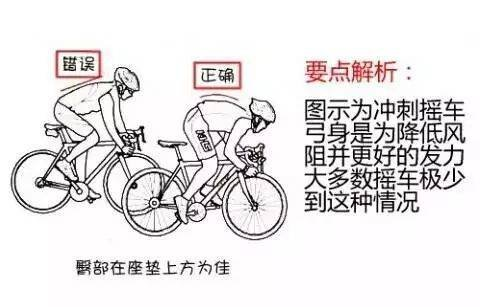
\includegraphics[width=7cm]{fig/摇车4}
\end{figure}

什么时候不宜摇车
\begin{itemize}
\item 砂石路面
\item 弯道
\end{itemize}
新手摇车常见后遗症
\begin{itemize}
\item 腰酸:这个原因就是没有摇到位过早提起所造成的。摇车时候应该两边脚踏都要最大程度让双腿打直,脚踏踩到底。一方面最大发力,另一方面可以减少腰肌的劳损。
\item 膝盖酸:分前脚膝盖和后脚膝盖(踩踏的脚为前脚)。

如果是前脚膝盖酸,体现为踩踏时觉得酸。这个是也是由于摇车不到位所致,双腿没有充分打直,脚踏没有踩到底,力量没有完全释放。只注重双腿助力,而忘记了要将体重的力量也压下去,双膝蜷着没有完全爆发。

如果是后脚膝盖酸,体现为脚在后面往上回时觉得酸。表示用力方式不正确,正常来说后脚几乎是不用力的。
\end{itemize}
\section{xc}
\begin{itemize}
\item 挡位需调小,防止某些坑或障碍踩不动急停导致摔车

\item 重心靠后一些,颠簸路段不能坐在座上,遇到急陡坡重心需要再往后靠。

\item 没走过或者不熟练的路段速度不能太快,但是也不能太慢,太慢会降低通过性,就比如说有的大坑会被卡停。

\item 刹车前刹为主,后刹为辅。不可急刹,急刹前刹会翻过去,后刹会抱死打滑,打滑了也不要慌,马上降低刹车力道就可以了。刹前刹如果比较用力重心需要相应往后移。一般情况是带一点后刹控制速度,转弯或者颠簸需要减速的时候用前刹快速减速。

\item 路线的选择很重要,好的路线会轻松不少,但是要对你的车在这个速度下的机动性足够了解,到不了的路线不能强求,不太好的路线有时候颠一下也就过去了。

\item 四肢要松弛有力,就是时刻准备接受冲击的状态,但是一旦感到冲击要发力去支撑住,尤其是手臂,一旦支撑不住有可能会造成非常大的重心前移,在陡坡上很可能导致翻车。四肢是你的第二套避震系统。

\item 注意力一定要高度集中,越野路段的摔车几率比平路高上不知道多少倍,摔车出去的一瞬间不要慌,可以的话最好人车分离,因为车上的一些边角还是能造成一些伤害的,尽可能保护好自己,在地上打个滚是个比较好的缓冲方法。
\end{itemize}
总结:不行就推车

篇幅有限,不能详尽说明,如果对越野有兴趣的小阳光可以去看《山地车圣经》,车协有电子书资源。
\section{过隧道}
\begin{itemize}
    \item 打开车灯,过隧道结束后要及时关闭
    \item 取下骑行眼镜/墨镜
    \item 拉开车距
    \item 如队伍过长,建议分队通过,每队三到四人。这是为了方便机动车超车
\end{itemize}
\chapter{骑行事项}
\section{基本准则}
\label{sec:基本准则}
\subsection{队伍队列}
\begin{itemize}
    \item 保持队形整齐,车距合适
    \item 原则上,全程队员严格听从前骑指挥,紧跟队伍行进,遇突发紧急情况时,队员要及时变通反应
    \item 视线保持在前方稍开阔,勿低头盯前车轮胎,勿左右分神
    \item 严格遵守交通规则
    \item 身体或车辆有任何异常,及时向队长或队医或后骑反映,并缓慢减速小心离开队伍解决
    \item 骑行时双手握紧车把,禁止放开双手,禁止手搭在车把上
    \item 若有人摔车,仅队医,其中一个后骑留下,其他人绕过并跟随大队伍继续前行,不得做多余停留。
    \item 有任何情况需要骑出队伍的,跟周围人打好招呼,并做出对应手势,仅后骑留下陪同。两列时,外侧人骑出队伍左侧,右侧人骑出队伍右侧,缓慢减速,让队伍正常通过。注意来往车辆!
    \item 需要归回队伍当中的,应做出相应手势,看到手势者应主动配合减速。
    \item 在保证自身安全的情况下做出骑行手势,但所有人口号必须喊到位(包括从前往后传和从后往前传),车技不好可以不做手势。
    \item 仔细阅读安全协议,严格守时守信。所有集合时间均为做好一切准备达到可以随时出发的状态。
\end{itemize}

按照以上规则,根据队长和前骑的要求在团队里骑行。(队形整齐,行进平稳),队伍行进过程中所有人听从前骑和队长指挥,不得指责前骑,若有建议,跟队长商量。

\subsection{踏频与档位}

就是一分钟以内脚踏所转动的圈数。对于骑友来说,骑行中保持一个有效踏频,省力,而且速度快。而且,有效合理的高踏频骑行,对膝盖的压力也是最小的,同时高踏频骑行还能起到瘦腿的作用。

30速的车子,你可以设置成2/6,2/7或者2/8,甚至2/9的档位,前提是你的体力跟得上踏频的运转。

踏频频率很高的话,它也一样会对你的关节有所影响,比方说当你的腿部运动达到每分钟超过83转的踏频,时间久了都会对膝盖都会产生一定的磨损。

\subsection{平路骑行}
\begin{itemize}

    \item 注意力高度集中,视野稍微放开阔,注意前骑或前方传来信号,

    \item 对突发情况能及时做出反应,减速或者加速,紧随前方步伐,切忌慌张

    \item 遇左右有障碍物如护栏,路沿,停放车辆等,要及时避让保持左右距离并提醒其他人

    \item 遇反向行驶或后方来车要减速避让,若两边均来车情况较乱首先稳住自己,再提醒他人 

    \item 两列骑行时,若遇路变窄难以通过(前骑未发出变一列信号),要主动与旁人沟通临时变一列通过

    \item 队伍超车时,紧跟前骑加速,从一旁绕过(超过后注意勿立马减速或挤到前面)

    \item 时刻做好捏后刹准备,一般减速只用后刹,禁止突然无故减速,禁止捏死刹车(尤其前刹),禁止只捏前刹(紧急刹车时应先捏后刹,再捏前刹)

    \item 遇路边公交车临时停靠,需要超车或等待,听从前骑信号而定,超车须果断跟紧(一般前骑会根据队伍当前速度和公车停靠时间等情况合理选择,队员需信任和服从),若遇公车强行加速果断减速避让

    \item 若遇外来车辆强行破坏队伍,要果断避让,待情况稳定后还原队形

    \item 遇路口处,要停车提前换小几个档位以便可以快速出发 ,停车尽量靠右

    \item 路口处通过时要紧跟队伍,稍加速通过,勿拖拉,勿中途停留

    \item 常规速度路况骑行下队伍前后两人车距为半个轮胎至一个轮胎左右。下坡快速骑行下队伍前后两人车距在5m以上,根据前骑要求而定车速越快,车距越大。左右两人车距为一辆车宽。
\end{itemize}
总结:该怂得怂,该勇得勇,遵守规则,灵活应变,胆大心细,整体感强
\subsection{常见交规}
\begin{itemize}
    \item 左转
    
    如果有专门的左转灯,当左转灯为绿灯时,由后骑负责拦左后方右拐的车辆,其他人正常左转。这种情况不建议把左转拆解成两次直行,即耽误了时间,更重要的是第一次直行之后,队尾需要摆到另一边,十分不便。

    如果没有专门的左转灯,应将左转拆解为两次直行。
    \item 直行
    
    当直行灯为绿灯时,由后骑负责拦左后方右拐的车辆,副前骑负责拦右前方右拐的车辆,其他人正常直行。

    特别指出,当路口为丁字路口时,即使直行灯为红灯,无需停车,适当减速即可通过
    \item 右转
    
    一般可直接右转
\end{itemize}
其他路口,根据具体信号灯指导走
 
交通标志:非机动车道和机动车道标识

有非机动车道的,一般禁止骑出非机动车道左侧白线外。(除非根据路况前骑选择临时占用机动车道,应跟随前骑)

队伍骑行禁止长时占用机动车道,禁止上高速,或无非机动车道的高架桥。

无明显非机动车道的,尽量靠右行,注意路边路沿。
\subsection{口号说明}
\begin{itemize}
\item 准备好了吗(没准备好吱声,准备好的人重复''准备好了吗``,都准备好之后最后一个人说''好了``,防止混乱)
\item 减速
\item 加速
\item 人齐了吗(答语:齐了/没齐,缺xx个)
\item 一列/两列
\item 坑
\item 小心
\item 左转/右转
\item 靠左/靠右
\item 减速带
\item 拉开车距
\item 扶好车把
\end{itemize}
关于手势

减速、靠边停车、加速、插入、右转、左转、我不行了(我车有问题了)你先走

口号一定要大声传给后面的人。

队形变换手势和口号由前骑发出,一列变两列时,队伍前部分适当减速。两列变一列时队伍前部分适当加速。一定和附近队员商量好谁前谁后。队形变换过程要求快而整齐。
\section{骑行职务}
\subsection{队长}
队长不要忘了安排人带防潮垫!!!


队长,乃一队之首,较之古之一县之长乃至一国之君有过之而无不及,时而不容有犯,不怒自威,时而需无操卖萌,掌握万千游戏之精髓,时而有如队员之父母,事事虽毋须躬亲,定要虑入牛毛之微。

总的来说,队长的工作包括,策划活动,安排活动,领导队伍,维持秩序,活跃气氛,关键决策。作为队伍的核心,队长要胆大心细。能一本正经的干正事,也能让每一个队员都感到温暖和快乐。

\textbf{活动前:}

\begin{itemize}
    \item 策划
    \begin{itemize}
        \item 新老队长对接工作;
        \item 参考之前的策划,尽量要有自己的创意,根据实际情况,如夏季还是冬季,新人较多还是老人较多等酌情更改策划;
        \item 景点还要考虑门票、学生证、身份证、集合时间地点等问题;
        \item 如之前没有过类似活动,需搜索目的地究竟哪里比较好玩,条件允许的话拉着前骑后骑探路,熟悉在哪休息,车子放哪;
        \item 路线、路况、难度、对队员和车况的要求、建议、景点介绍、主要流程安排、队长及队长联系方式;
        \item 做大致路线图;    
        \item 最迟周日中午12点发在群里;
    \end{itemize}
    \item 宣传
    \begin{itemize}
        \item 在q群和微信群提前宣传,将策划最精华的部分拿出来,整理语言,在群里宣传招募队员;
        \item 转发推送,拉人参加;(主页君和主页妞也要转发)
        \item 队长要多参加晚训和大家混熟,还要在晚训时宣传活动内容;(对于难度大、危险系数高的活动可以进行强调并劝退;)
    \end{itemize}
    \item 安排事务
    \begin{itemize}
        \item 周三晚报名截止后领取初始活动名单(找办公室索要),初步安排职务;
        \item .联合办公室统计未晚训人员并督促补训;(补训事宜:上周五,本周一三均有上课等正当理由不来参加晚训者可以予以补训,队长需到场检查,严禁周五补训。)
        \item 统计借车人数并向实践部反馈;
        \item 统计借头盔人数并向实践部反馈;
        \item 统计借或买手套手套的情况;
        \item 周三晚上报名截止,两名队长协商制定职务,于周四中午之前将名单发送至办公室;
        \item 提前与老队员进行沟通安排职务;前骑X2,后骑X2,均为老带新,大旗X1,队医,摄影X2,队记X2,建议男女各1;根据路线特点决定是否安排后助。职务安排参见职务工作要求,以队员体力能力为首要参考,报名意愿为辅助参考;
    \end{itemize}

    \item 检车

检车前一天晚上发短信通知检车事宜。


时间:周五中午12点30分

地点:东区:车棚;

      西区:7号楼与8号楼之间的空地;

流程:
    \begin{itemize}
        \item 签到—办公室负责,每人领取策划;
        \item 借车—队长通知实践部带领借车人员前往车棚取车,并填写租车信息登记表,提醒办公室收缴保险费;
        \item 队长发言—检车基本完成后,将所有队员聚拢,手持策划具体介绍活动;(强调出发集合时间地点;介绍活动强度及特色;团队骑行纪律、交通规则、和骑行安全等注意事项;关于安全协议,所有人必须签字在出发前上交;讲明迟到后果)
        \item 向所有人介绍前骑,后骑,队医;
        \item 对全体队员进行骑行手势,口号教学,对不会骑车或者不会换挡的进行现场教学,现场试骑车辆;
        \item 检车—队长安排实践部带领并现场教所有人检车修车;(刹车灵敏度,快拆杆松紧,前叉能否解锁,坐垫高度,变速换挡,链条传动系统是否生锈需要上油,轮胎气压)
        \item 租借头盔的领走头盔。

        \item 检车完成后所有人把车放回车棚并解散;
    \end{itemize}

    \item 出发前
    \begin{itemize}
        \item 活动前一天晚上再次通过微信或短信通知所有人出发集合时间地点以及注意事项;看看天气预报,如有雨雪需提醒队员携带雨具;

        \item 提醒前骑提前熟悉路线并发路书至微信群;

        \item 提醒后骑配好完整后骑包后骑拿后骑包看路线;

        \item 安排人带防潮垫及绑绳、桌游、雨衣等;

        \item 提醒大旗拿大旗绑绳旗杆并在出发集合前绑好;

        \item 提醒并确认队医配好队医包;
    \end{itemize}
\end{itemize}

\textbf{活动中:}

\begin{itemize}
\item 出发集合时收齐安全协议,到点准时点名;
\item 队长跟在队伍中后方以及男女生分界处,督促队伍队形整齐,口号响亮,手势规范及时,发现队员任何异

\item 对违反安全协议的队员及时予以纠正。

\item 适时与前骑沟通情况,安排队伍休息。

\item 路上出现队员摔车、体力不支队员掉队、车辆出现故障掉队的队员,应让其出队减速等待后骑帮助,并提醒队伍超越他并跟紧前队。

\item 在目的地游玩或坡顶休息的较长时间里队长要主动带领大家或让车协老人带领大家进行游戏活跃队伍气氛。

\item 根据队长和前骑的要求在团队里骑行。(队形整齐,行进平稳),队伍行进过程中所有人听从前骑和队长指挥,不得指责前骑,若有建议,跟队长商量。

\item 若有人摔车,仅队医,其中一个后骑留下,其他人绕过并跟随大队伍继续前行,不得做多余停留。
\item 队伍在坡顶集合后,队长集合所有队员强调注意事项,安排后骑带领大家检车,主要检查刹车性能、检车前后轮快拆轴、检查头盔是否正确使用;

\item 强调放坡规则:前骑根据路况控制速度;队伍一列放坡;车距保持在1~2辆车的距离;禁止超车;口号喊响亮;队伍最后是后骑、大旗、队医。
\end{itemize}

具体骑行规范请看第 \pageref{sec:基本准则} 页。

\textbf{活动后:}

\begin{itemize}

\item 活动结束后,队长需选择合适的地点和时间召集所有队员开会,进行职务总结和队长总结,包括工作总结,对问题的指出和批评,对优良表现的鼓励表扬,要求简明扼要,条理清晰,指出骑行中出现的问题,交流心得。
\item 多日活动须在开会时对第二天的进行职务安排,路线熟悉等。
\item 活动结束回到学校后,队长需要安排人对所有租借的车辆进行检查和适当维修,将情况如实汇报给实践部部长,实践部部长再将车辆情况反馈给车主。
\item 如出现车辆较大损坏,实践部部长和队长需要协助借车的队员联系车主商议修车或赔偿等事宜。
\item 提醒队记,摄影,迟到者的检讨等文件活动结束后第二周周三前整理并发送至微信群或q群;相应文件发送到QQ群相应文件夹;(队记、队长总结发送到执委群,图片视频发送到7群)
\item 活动结束后三天内,队长需要提交队长总结,总结内容须包含:骑行总结、职务总结、摔车情况、个人心得、攻略提示等,切忌流水账。
\item 督促租借头盔的队员清洁头盔,并回收交至实践部。清洁方法见\pageref{sec:头盔清洁} 页。
\end{itemize}

\textbf{迟到:}

\begin{itemize}
\item 检车

    队长点名签到,检车开始,不允许迟到。

    若未提前与队长说明原因,迟到10分钟以上将取消当周活动资格。

    检车请假的队员须在活动前与队长约定其他时间于活动前完成检车相关流程。
周末骑行活动出发

\item 活动

    迟到10分钟及以内写1000字以上书面检讨,并罚跑一定圈数或对车棚车辆进行擦洗。

    晚吃饭30s。

    迟到10分钟以上者取消活动资格,同样处以上述惩罚。

    报名活动后无故不参加活动者将被拉入车协黑名单,取消之后活动的报名资格,如想继续参加活动须向阳光车协理事会提交申诉,由理事会观察讨论后决定。
\item 多日骑行及暑期远征

视情况由队长决定处罚办法。

\end{itemize}

\textbf{安全协议及免责声明:}

\begin{itemize}
\item 活动前签到,所有队员须将免责声明上交队长,未上交将不允许参加活动,活动后由队长将全部免责声明交到办公室统一保管。

\item 活动时队内若有人违反安全协议相关内容,队长有权进行批评与纠正,若队员不听劝阻多次违反相关规定,队长有权将其请离队伍并送回学校,并限制其日后参与协会活动的权利。

\item 阳光车协理事会对安全协议及免责声明拥有最终解释权。
\end{itemize}


\subsection{前骑}

带队按计划完成活动路线。

\textbf{基本要求:}
会看地图,体力够好,懂基本交通规则,为队伍着想,一般为男生。

\textbf{活动前:}
\begin{itemize}

\item 路书:

活动前一天做出路书,制作方法见 \pageref{chapter:路书制作方法} 页。

不要单纯使用行者做路书,因为一些封路的路段行者不会实时更新,参考高德地图骑行导航制作。拒绝上路直接导航,标出途径点和休息点,优先找有卫生间和商店的地点,如我们的好兄弟加油站。一般骑行20公里左右或者1小时左右休息一次。

路书需要发至活动群确保所有人能看见。

\item 装配:手机支架、码表、充电宝。

\end{itemize}

\textbf{活动中:}
\begin{itemize}
\item 要熟悉路线,骑行过程中对路线有疑问时,可以和队长打招呼后离开队伍,加速去前面探路,或是选择合适地点,全队休整,打探路线。

\item 应对路况车流等情况,通过灵活运用手势口号和调整队伍速度及时躲避车辆、障碍和坑。如:前方遇到减速带,则稍减速并大声喊口号提醒前方减速带;迎面右侧或左侧有逆行车辆,则提醒队伍靠左或靠右躲避。用手势传递信息与后骑和大旗配合在必要时刻拦车。

\item 前骑要控制好时间,一般情况下,连续骑行一小时左右休息十分钟,休息地点常选择有厕所的地方如加油站或是商店。休息地点要宽敞,提醒队员摆放车辆。

\item 两个前骑应提前做好沟通和明确分工合作,分一列还是两列骑行。道路狭窄或道路变宽:加速并通过手势及口号提示队伍变为一列;减速并通过手势及口号提醒队伍变为两列。

\item 前骑需要在一天的活动保持极高的专注力和应变力,设定两个前骑相互辅助相互提醒,心中责任感要强,当遇到突发状况时,一定要保证队友也可以通过再前进,切忌急刹车!!!对实时路况做出快速反应,并为后方队伍传达信号。

\item 多喊口令,前骑比所有人的视野都开阔,需要把路上可能遇到的危险告诉后方的队员。当遇事不决,不知道该怎么处理时,喊减速。

\item 骑行时要及时了解队形,在回头看队伍之前一定要先看前方,确保安全,双前骑时配合要有默契,一个往前看,一个往后看,忌同时往后看;注意前方车辆的转向灯等。

\item 前骑控制好速度,要保持匀速,忌忽快忽慢,并根据骑行时间、温度、路况、队员状态及时灵活的调整速度。骑行时要等所有队员归队时再加速。

\item 不定时回头看队伍,路口处,前骑注意来往车辆(外侧前骑注意左后方右转车辆和左前方左转车辆,右侧前骑注意右后方左转车辆和右前方右转车辆)必要时,留一个前骑拦住对应车辆。另一个前骑带队伍通过。严格遵守交通规则!!!

\item 前骑方位感要强,会利用一些参照物推理出正确方向,善于利用路碑、路标等外物,不要依靠手机导航;有队友超越前骑时,要及时指出,开会批评。

\item 视野要开阔。前方有障碍绕行时,根据速度及队伍长短选择合适的距离打出手势,绕行时一般从左边绕行,绕行前要看后方有无车辆,是否有足够的时间来完成绕行;过公交站有公交上下人时一般要停止前进。前方有路口时,尽量提前看红绿灯,根据灯亮情况来调节速度,尽可能让队伍到交通灯附近时是绿灯,遇到红灯停车时,要尽量靠右停,避免队员''扎堆``堵路的情况,若停车时占右转车道,可根据情况将车挪至路口;过桥洞时要减速,观察洞外有无行驶车辆。''近看``''远看``,多数情况下目视距离偏近些,当后方有汽车驶过时要借助其灯光看远些,并记住所视范围内的路面信息(是否有行人、路况等)。

\item  团队爬坡和放坡适合控速,遇到扁担破提前提醒并加速,在坡顶等人并带队放坡,下坡时拉开车距。原则上整体放坡速度不应超过30km/h。
\item 到达休息点后,把位置发至活动群,方便掉队的人追队。
\end{itemize}
\textbf{活动后:}

活动总结。
 
\subsection{后骑}

掌握修车技能,体力较好,会看地图(至少会导航)。

\subsubsection{具体工作:}
\begin{itemize} 
\item 修车

路上任何时候队伍中出现车辆故障后骑要第一时间予以解决。

作为后骑,卸车轮补胎是基本功,大多数情况下,出问题都是因为扎胎。这种东西不通过实践来学习是不可能学会的,当次活动的后骑在检车时要多向老人请教,比如如何不蹭碟,如何换刹车线,变速线,来令片。

每支队伍的两个后骑各带一个后骑包,活动前一天配好,确保工具齐全。

后骑包:补胎工具一套:磨胎棒一根、撬胎棒3根、补胎片10个左右;补胎胶一支、组合一套、气筒一只、备胎27.5和26各一个(注意统计一下嘴型)、截链器一个、来令片一对。

\item 拦车

队伍外侧后骑应骑出队伍半个身位以便观察完整队伍以及前后来车。后方来车时及时向前骑传口号。配合前骑在必要时拦车。(尤其队伍需要左转)

\item 检车

放坡前,后骑帮所有人检车(刹车,快拆,解锁前叉,档位调大)。

\item 认路

很多人都以为认路是前骑的事,所以活动前后骑就不是很关心路线,根据活动结果来看,后骑不认路会严重影响队伍的前进速度,也会给队长和你陪的人更多的心理压力。所以每次活动的后骑要多向前骑询问路线,做到掉队后可以找到队伍。

\item 陪人

有人掉队后骑其中一个留下,保证有一个后骑跟随大队伍。车坏了熟练修好车,骑不动了要和人聊天做心理工作(讲故事吧)。

陪掉队人员时,后骑负责带路追上队伍,因此后骑需要了解路线会带路。

陪人是后骑的天职,不管你愿意还是不愿意。掉队在平时活动和拉练中都是无法避免的事,一个优秀的后骑会给掉队的队员安全感。因此,后骑往往还需要掌握尬歌,没话找话等能力。

\item 杂活
    \begin{itemize}
    \item 收垃圾:准备若干袋子,在休息时收集队员制造的垃圾并及时清理。
    \item 捡东西:若前方队伍有人掉落物品,后骑留下捡起。
    \item 查房:因为前一晚很累,第二天难免着急丢下自己的东西,所以在集合后后骑要去各房间检查,找到落下的东西后对主人提出批评。
    \item 查饭桌:检查饭桌及周围有无落下东西。
    \item 转桌子:转桌难道会影响抢饭??
    \item 查车:在多日骑行活动中,当天骑行结束,应当去检查每个人的车是否正常(主要是检查胎是否漏气)。
    \item 补胎:当天晚上补当天破的胎。
    \end{itemize}
\end{itemize}

\subsubsection{注意:}
\begin{itemize}
    \item 注意检查后骑包每个工具能否正常使用,如打气筒漏气否,截链器之前有没有损坏过链条。

    \item 要对破胎做好标记,避免当天晚上补胎的时候不知道是哪个胎破了。

    \item 在路上遇到胎破了的情况,不要就地补胎,会很浪费时间,换上备胎继续前行。在当天晚上,后骑要把胎补好交给第二天的后骑。

\end{itemize}

\subsection{前站}
\begin{itemize}
\item 配置:体力好、嘴皮子好、认路、尽量几名男生配合一名女生。
\item 流程:
在队伍需要统一找餐馆吃午饭、晚饭、住宿时发出。

在距离目的地约30分钟骑行距离时队伍停下整顿,队长指定2-3人打前站,随后队伍休息。
 
前站需以较快的速度尽力飞奔到目的地,挨家挨户了解吃饭住宿情况,衡量价格条件,并合理安排分房,妥当后尽快联系队长。摆好碗筷,倒好水。在队伍到达时,及时迎接大部队。

\item 注意事项:一般不要点饺子,面此类自己吃的东西。

\end{itemize}
前站:在离终点一定距离(一般为一次骑行的距离)提前出发为队伍寻找食宿地点的小队,2-4人,要求体力较强。

前站根据预算找好吃饭地点,点好菜并发位置给大队伍,在队伍到来前排好座位,倒好茶水,并安排人在路口显眼处接待大队伍,安排好停车。安排住宿时,队长收齐所有人身份证交给前站。前站安排晚上队员的住宿分配,按新老混合,随机分配原则。一般先安排住宿再通知所有人集合去吃饭,迟到有小惩罚。
\subsection{队医}
队医

一、须掌握必要的运动伤害处理技能,有耐心细心。

二、熟悉如何配置队医包以及队医包内所有药品物品的使用方法。

三、有队友摔车受伤或出现其他意外情况应及时上前处理。

四、在团队放坡时主动到队伍后方后骑前面。



\subsection{摄影与队记}
其实每个人都可以写队记,拍照片。专门安排职务的目的是避免出现恰好所有人都没有写队记,拍照片的情况。

照片和文案之后会在活动回顾的推送中用到。特别好看的照片还会被印成明信片。

照片和队记要及时上传至QQ群。
\subsection{大旗}

注意限高啊!!!

有大旗代表有车队,大旗需紧跟队伍。选择体力好,车技稳的人。

\subsubsection{位置:}大旗应在团队最后方靠近汽车道位置,向外飘出半个车位,前骑通过大旗的位置确定队伍整齐度和团队情况。

\subsubsection{具体工作:}
\begin{itemize}

    \item 骑行集合时间前把大旗绑好,提前去办公室拿绑绳和旗。

    \item 协助后骑向前传达口号以及拦车。

    \item 休息时,若后方还有队伍或者掉队人员,大旗把车停在休息点路口外显眼处,以便后来者发现。

    \item 拍合照时,大旗及时拿旗。

\end{itemize}


\subsection{心理委员}
心理委员一般只有在暑期远征或冬训的时候才会安排。在长途骑行中,往往会出现很多问题,容易出现自闭的现象,因此,会安排一名心态极好的同学来做心理委员。

尽可能在问题产生之前就及时沟通,解决问题。
\section{意外情况处理方案}
\subsection{掉队}
掉队不是什么大问题啦,当队员实力低于路线难度的时候是很自然发生的事情。碰到这种情况,需要一个后骑跟在队员的身边陪ta一起掉队。

当大部队到达休息点时,队长应当主动联系掉队的人,了解后面的情况。
\subsection{摔车}
当队伍发生摔车,一个队长,一个后骑和队医需要靠边停下陪同摔车者,并对摔车者进行初步治疗。

前骑应该适当减速,但是不要停下!不要停下!不要停下!在附近找一个临时休息点(一定不能是路边这种不安全的地方)等待掉队人员追上。

如果摔车者伤势严重,队长需要给前骑打电话说明情况,在需要的情况下应当将摔车者送往医院。


\chapter{路线总结}
\section{A级路线:夜间}
\subsection{夜游京城}

路书编号:2906265,2906268 路书上连不起来所以分成两部分

\begin{figure}[htp]
    \centering
    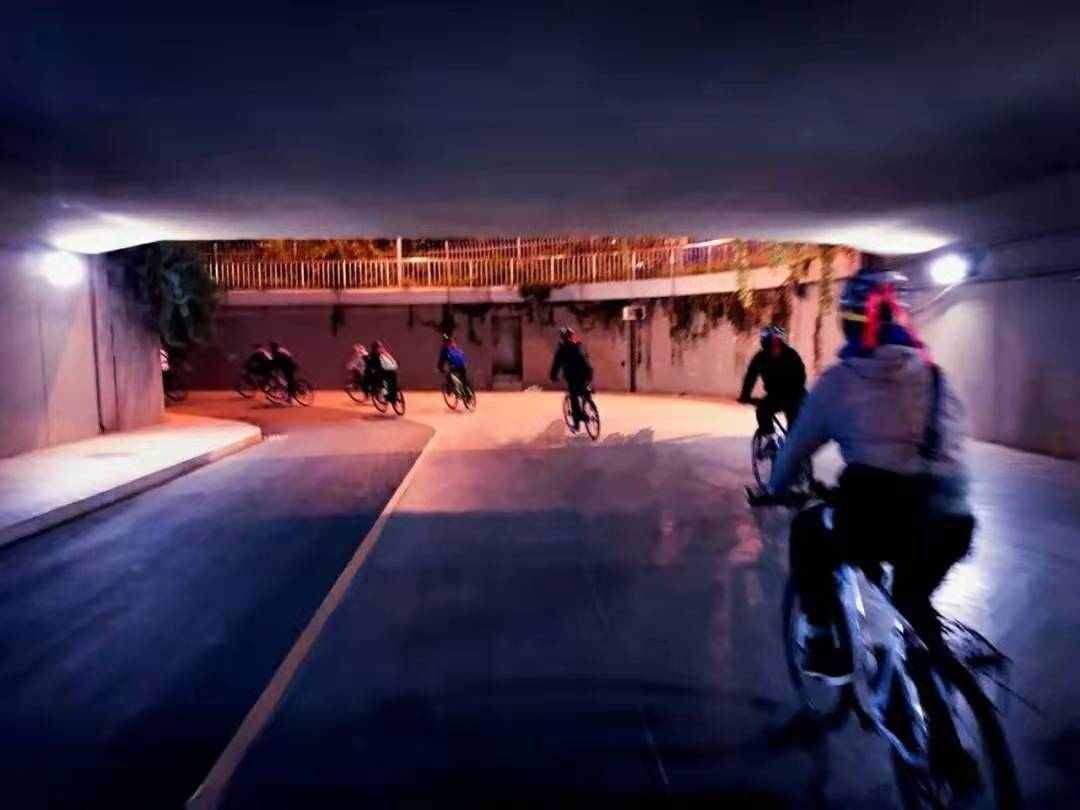
\includegraphics[width=0.7\linewidth]{fig/夜游京城1.jpg}
    \caption{图片摄于2020年10月23日}
\end{figure}

\begin{tips}
    夜游京城经常容易忘买保险,2021年和2022年都忘记买了,一定要叮嘱办公室买保险!
    \end{tips}

注意:在刷长安街前,要把队伍化整为零,不要所有人一起列队过去,更不要挂旗。其实夜游京城可以不带旗杆,只带一面旗子用于拍照。
\subsection{夜爬百望山}
\subsection{奥园刷圈}
路书编号:3033808 

奥园刷圈是一条经典路线。在这里可以偶遇很多大佬,汽车少,路宽(机动车路宽),非常适合刷速度。

但是也存在一定的危险性。危险性有三,一是需要上机动车道、二是车速较快,需要更好的控车技巧、三是奥园刷圈一般需要跟车,一旦发生急刹等突发情况,往往面临的就是连环摔车。

注意:

\begin{itemize}
    \item 路书中前往奥园的路上有一段路需要上立交桥。这其实是禁止自行车上的。如果介意的话,可以绕开。
    \item 奥园刷圈路段有一段是没有自行车道的,存在一定的危险性。事实上,即使有自行车道,在刷圈时一般也不会走,而是选择机动车道。
\end{itemize}

\section{B级路线:骑游}
\subsection{银杏林}
\subsection{凤凰岭}
\subsubsection{时间安排}
集合→骑行出发→到达凤凰岭→山脚午餐→登山→景点游览及小活动→下山→骑行返程

7:20东区一队出发;

8:08两队到达西区;

10:30到达凤凰岭;

10:55队伍进入凤凰岭景区开始游玩;

15:00全体到达休息点集合完毕;

15:04返程;

约18:30全部回到学校,队伍解散

\subsubsection{路书}
1269952
\subsubsection{注意事项}
\begin{itemize}
    \item 学期初的活动,提前队长培训。
    \item 强调口号,全面检车、教学,发飘带。
    \item 休息点在温泉村以及凤凰岭山脚下的小镇,大部队基本维持17~18的速度。
    \item 了解购票系统,可以关注凤凰岭公众号。
    \item 一般采用绕北线一圈的方式游玩,比较符合时间。
\end{itemize}
\subsection{八大处}
\subsection{十三陵}
\subsection{怀柔水库}
路书编号:2724293
\begin{figure}[ht]
    \centering
    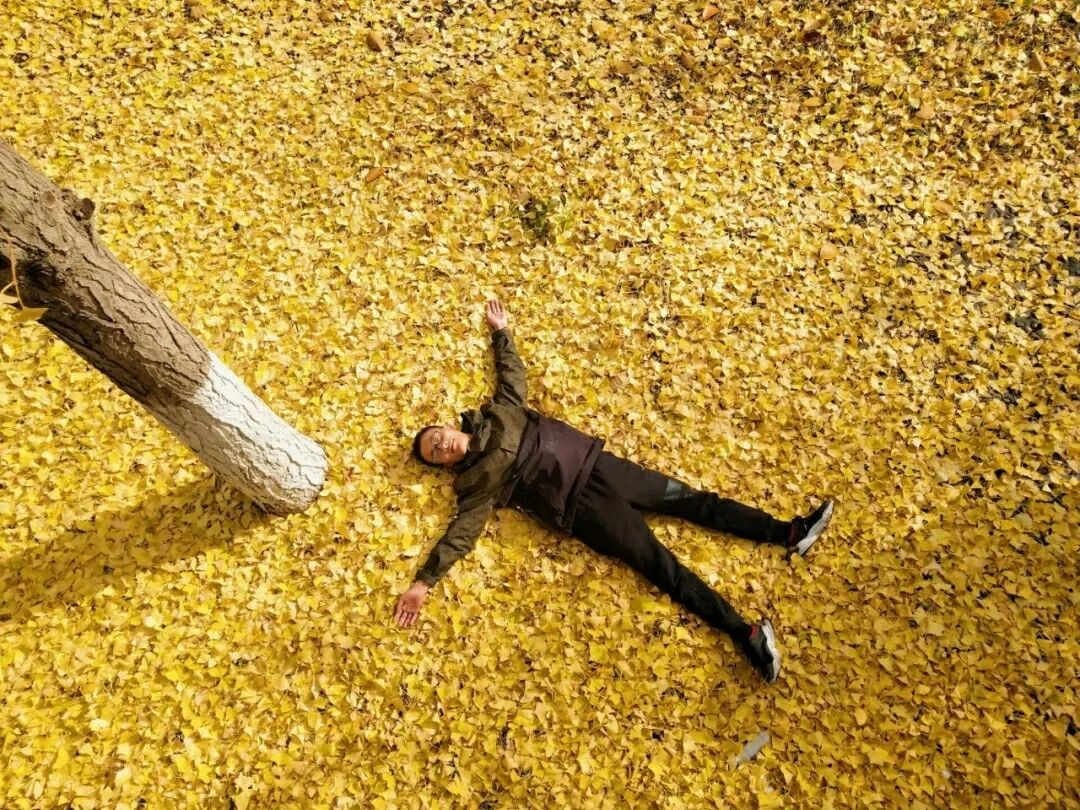
\includegraphics[width=0.8 \textwidth]{fig/怀柔水库1.jpg}
    \caption{摄于2019年11月10日 图中人物为2020届会长李琛}
\end{figure}
\section{C级路线:秋季拉练}
\subsection{太舟坞}
\subsubsection{时间安排}
2984345、2984347 这两段,参考用时5小时。(只计算了骑行时间,不包括开会,休息。集合)
\subsubsection{路书}
\begin{itemize}
    \item 农大东校区骑到太舟坞起点:3025598
    \item 从憋死猫xc放坡进入北京植物园(难度较大,推车情况比较多),几乎不存在反爬的可能 3025592
    \item 车协标准太舟坞路线:2984347(中间有一段连不上)。注意:中间需要抗车一次。另外,路况较差,而且有几个急弯,两边没有护栏,尽量避免傍晚放坡。
    \item 憋死猫放坡进入北京植物园:3025594。可以先从xc路线放坡下来,然后再从这根路线骑回憋死猫。
\end{itemize}
\subsubsection{注意事项}
\begin{itemize}
    \item 太舟坞的坡很陡,是容易前轮翘起那种陡,不建议安排在学期初期,容易劝退新人。
    \item 路比较烂,有行人,有急弯,两边有悬崖,无围栏,放坡的时候一定要小心小心再小心
    \item 中间有一段路需要把车抬过栏杆
    \item 最后大约有300m的究极陡坡,值得挑战
    \item 这也是车协唯一一个允许推车的路线
\end{itemize}
\begin{figure*}[!htb]
    \centering
      \subfigure{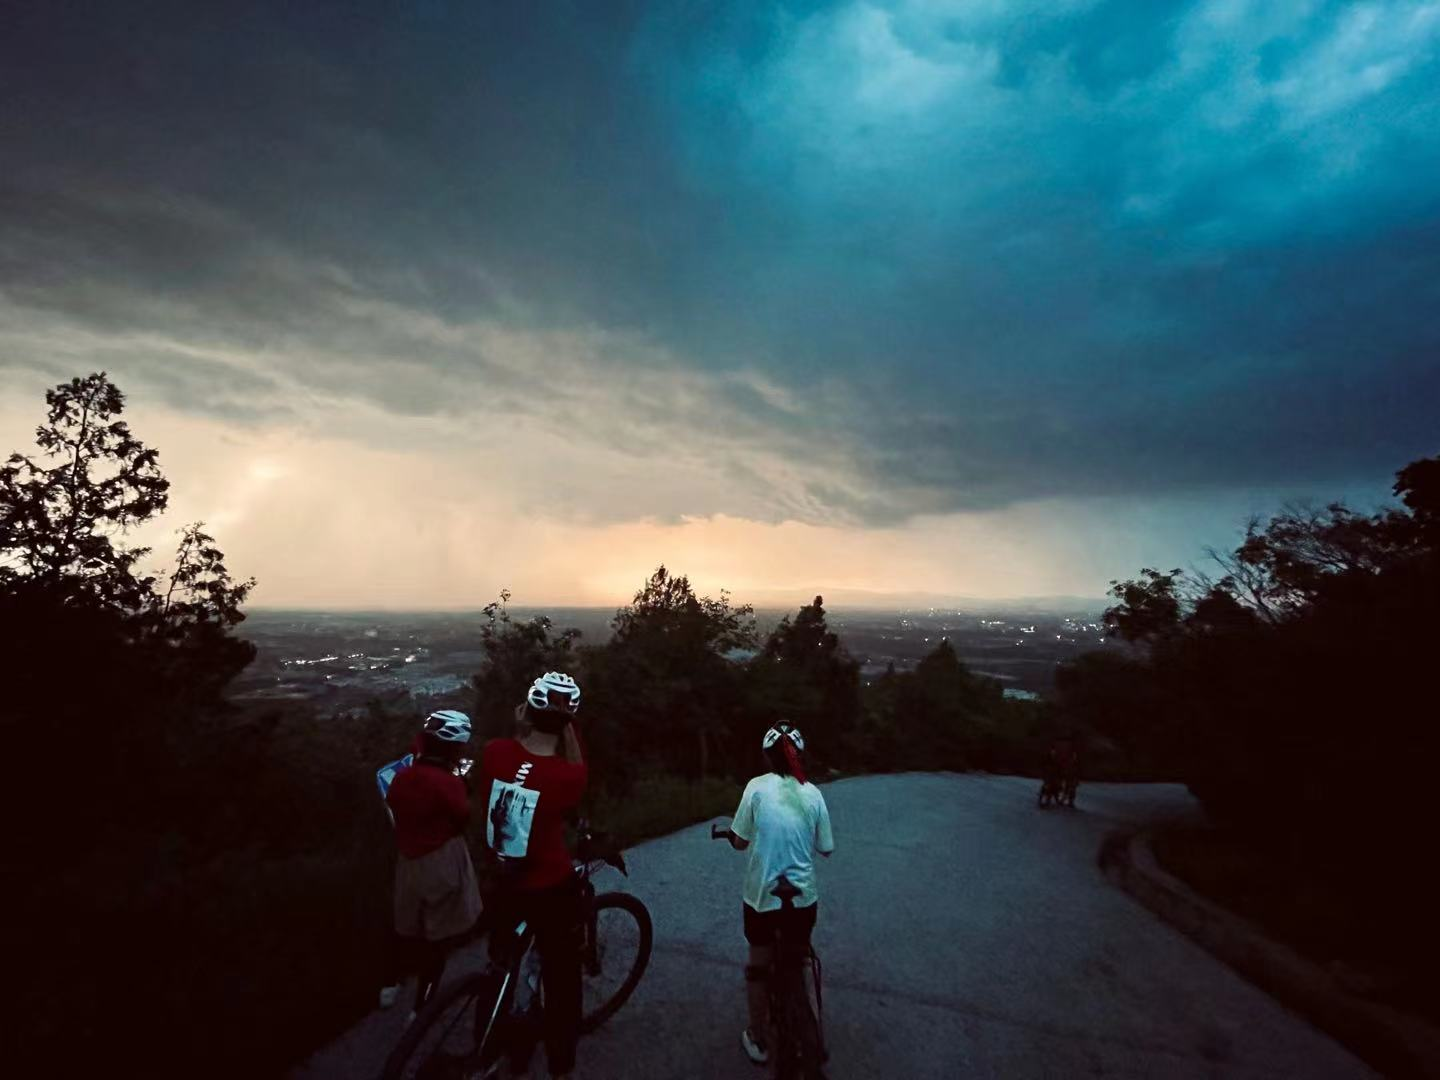
\includegraphics[width=0.45\textwidth]{fig/太舟坞2.jpg}} \quad 
      \subfigure{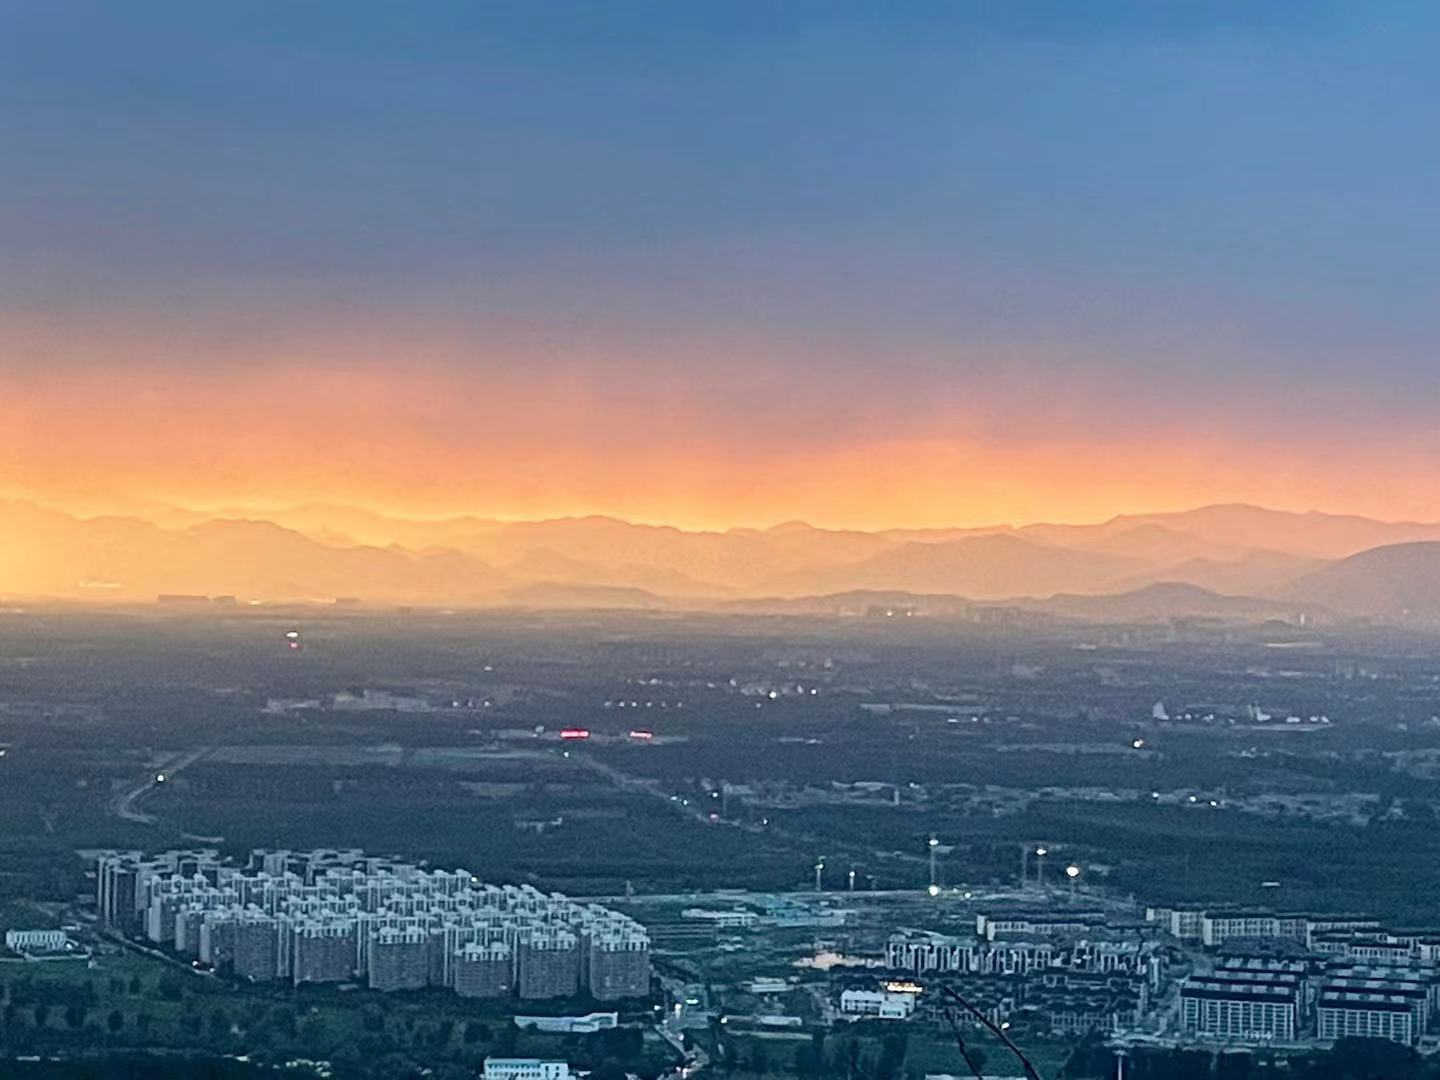
\includegraphics[width=0.45\textwidth]{fig/太舟坞1.jpg}} 
        \caption{拍于2021年6月30日}
  \end{figure*}
\subsection{戒台寺}
--斋饭时间
\newpage
\subsection{莽山}
\label{subsec:莽山}
\subsubsection{路线介绍}
路书编号:3100740,也可以直接用导航软件搜索,燕山文化广场,即可到达爬坡起点附近。

途中有两个容易走错的地方。
\begin{itemize}
    \item 上清桥,位于2km处。路书上看起来这里应该右转,但是这里应该选择中间的方向,随着这个方向往前走,最终会变成右转方向。另外,在选择中间方向的时候,应当选择中间车道。中间车道才是自行车道,右侧车道是对向来车的车道。
    \item 中央财经大学旁的高架桥,位于23公里处。这里要选择上高架桥,而不是下面。
\end{itemize}

从农大到蟒山,主要分成三段路:农大东(西)校区——辛庄桥加油站——燕山文化广场——蟒山山顶。其中第一段路为12km,第二段路20km,第三段路为爬坡路段9km。前两段路基本不存在因为体能掉队的可能。其中,辛庄桥加油站和燕山文化广场附近都可以找到厕所和商店,而蟒山山顶没有厕所和商店。

至于蟒山爬坡路段,9.2公里平均坡度5.2\%。其路段的坡度不是很均匀,开始1公里和最后1公里比较缓和,中间较陡,部分陡坡坡度可达到7-8\%。但是路况不是很好,会有一些坑洼,放坡时一定要解锁前叉。

之前去的几次都时间比较晚了,光秃秃的,也不怎么好看。据说在恰当的时候来,可以看到红叶。

另外要注意的是,蟒山半山腰是没有信号的,可以考虑带上对讲机。

爬坡前的燕山文化广场,有休息点,有厕所。
\begin{figure*}[!htb]
    \centering
      \subfigure{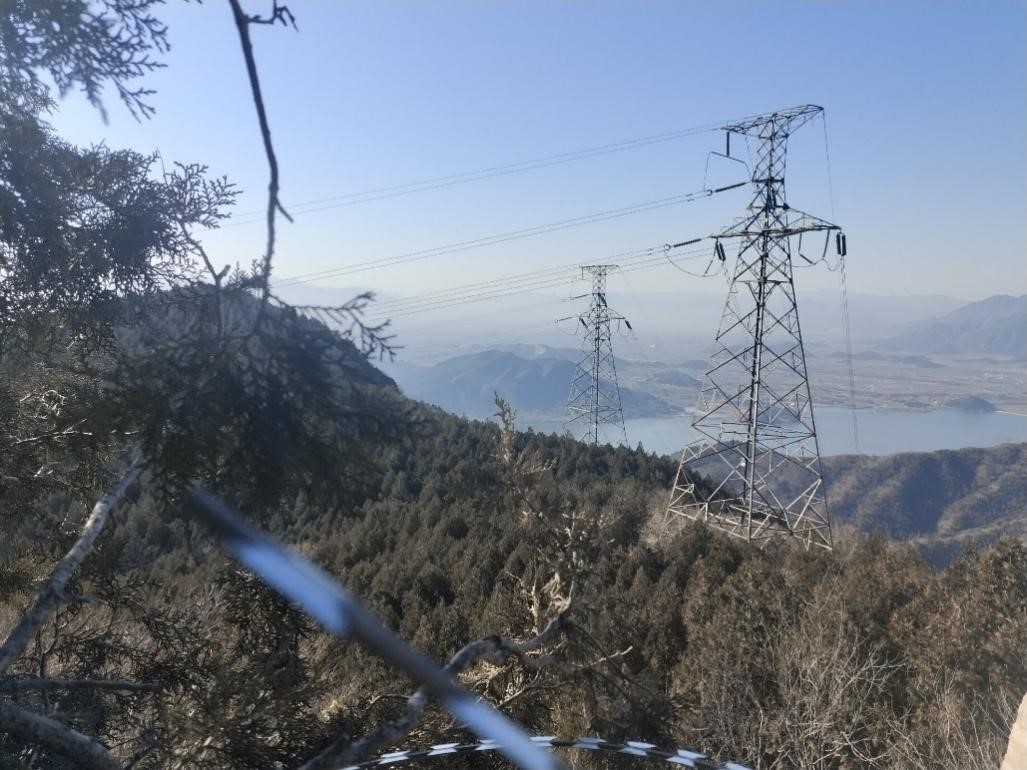
\includegraphics[width=0.45\textwidth]{fig/蟒山1.jpg}} \quad 
      \subfigure{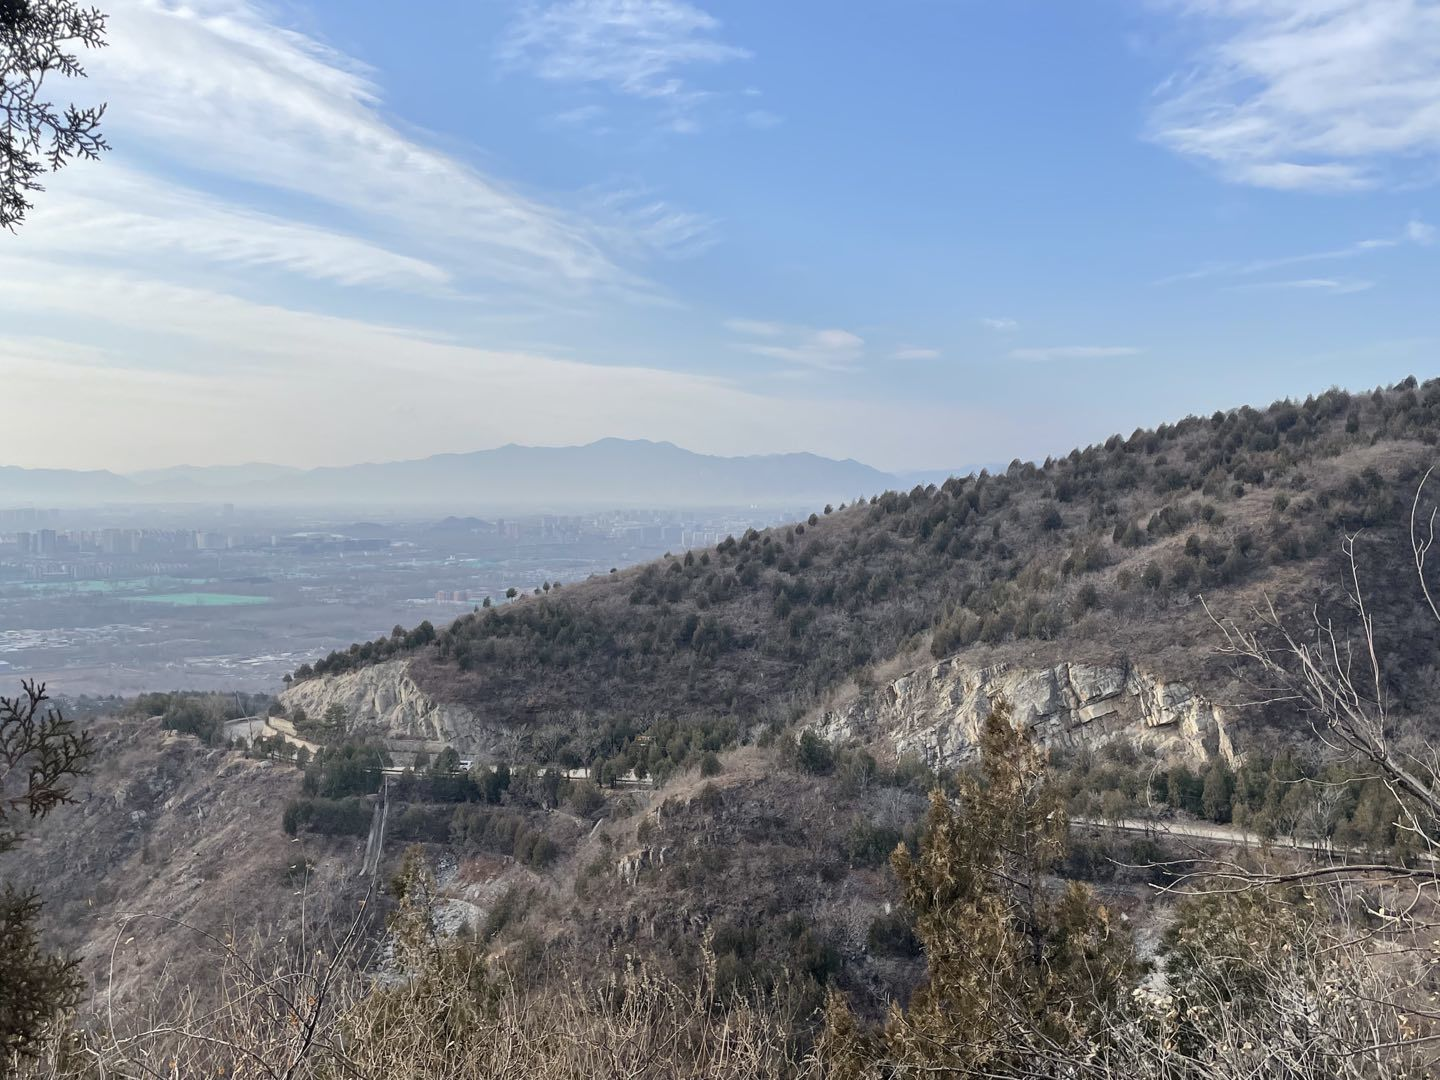
\includegraphics[width=0.45\textwidth]{fig/蟒山2.jpg}} 
        \caption{拍于2021年12月4日和2021年12月11日}
  \end{figure*}
\subsubsection{时间安排}

无论东西校区,前往爬坡起点大约需要2小时20分钟(在加油站休息15分钟左右的前提下)。爬坡路段,最慢的人大概需要90分钟(如果车坏了,还需要额外加时间)。

在2021年的冬训体测中,早上7点40出发,10点到爬坡起点,晚上4点半回到东区。

莽山作为2020/2021年的冬训体测地点,两次体测标准相同,均为男生60分钟女生70分钟。

\newpage
\subsection{大杨山}
路书编号:2915447
\section{D级路线:春季拉练}
\subsection{潭王路}
\begin{itemize}
    \item 路书编号:2982362
    \item 全长120km
\end{itemize}
参考时间:
\begin{itemize}
    \item 6点30出门:
    \item 预计晚上7点到东区
\end{itemize}
\subsection{禅妙阳连爬}
路书编号:2998176
\subsection{韭园}
路书编号:2998459

韭园可以算是暑期拉练的必有项目。主要是因为它可以让大家感受到更加复杂的地形,达到更加全面的训练目的。毕竟暑期路上并不全是好路。


\subsection{妙峰山}
\label{subsec:妙峰山}
路书:农大东区到妙峰山 \#3035456  \#

\begin{figure}[ht]
    \centering
    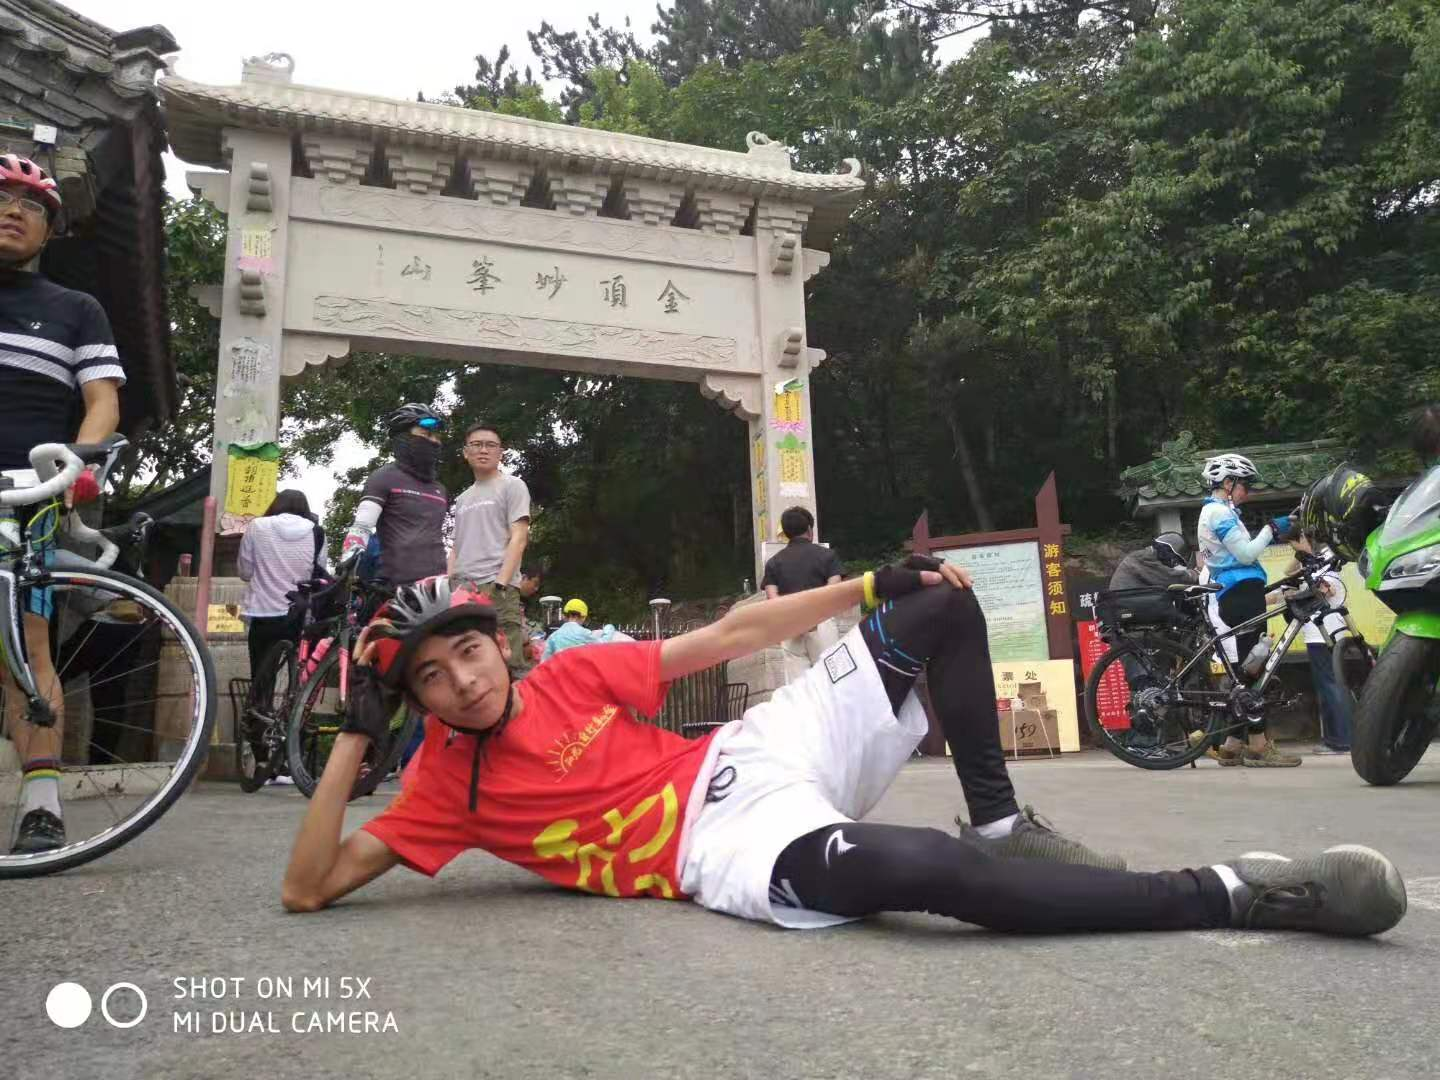
\includegraphics[width=0.8\textwidth]{fig/妙峰山1.jpg}
    \caption{图片摄于2018年5月26日,图中人物为2019届会长张焱辉}
\end{figure}

\section{E级路线:多日活动/特殊活动}
\subsection{黄花城水长城}
返程路书:2972779


\subsection{五一(赤壁山)}
路书编号:
\begin{itemize}
    \item 第一天1390541
    \item 第二天xc 2991897
    \item 第二天返程1400333
    \item 第三天2992783
\end{itemize}

\begin{figure}[ht]

    \centering
    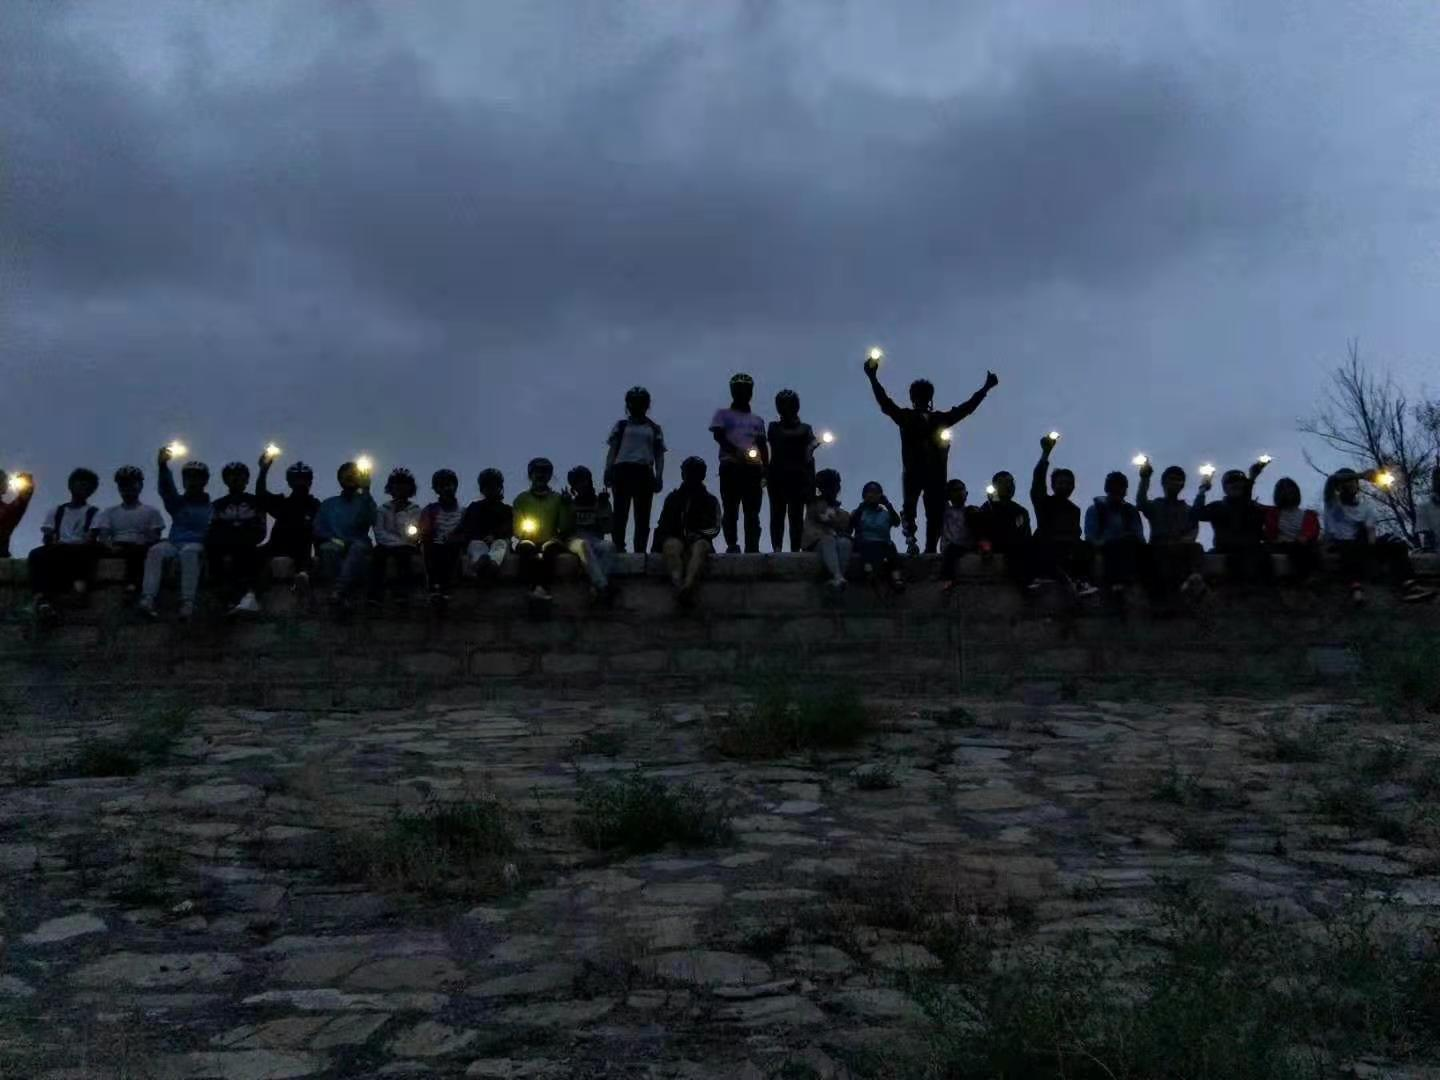
\includegraphics[width=0.3\textwidth]{fig/五一第一天2018年.jpg}
    \hfill
    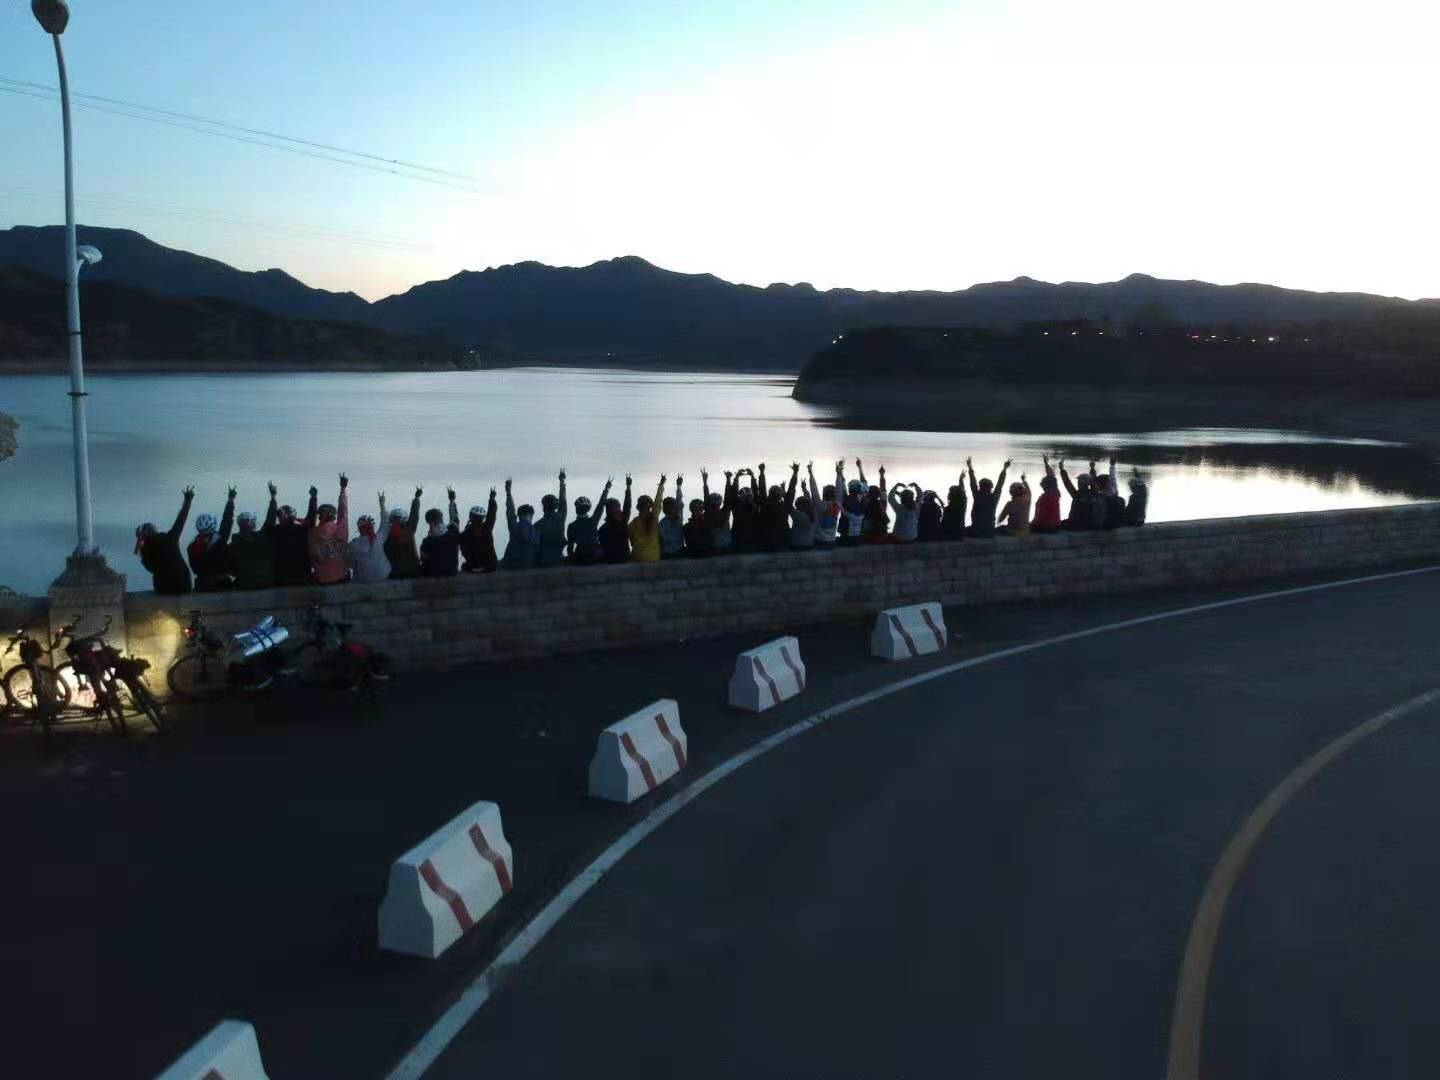
\includegraphics[width=0.3\linewidth]{fig/五一第一天2021年.jpg}
    \hfill
    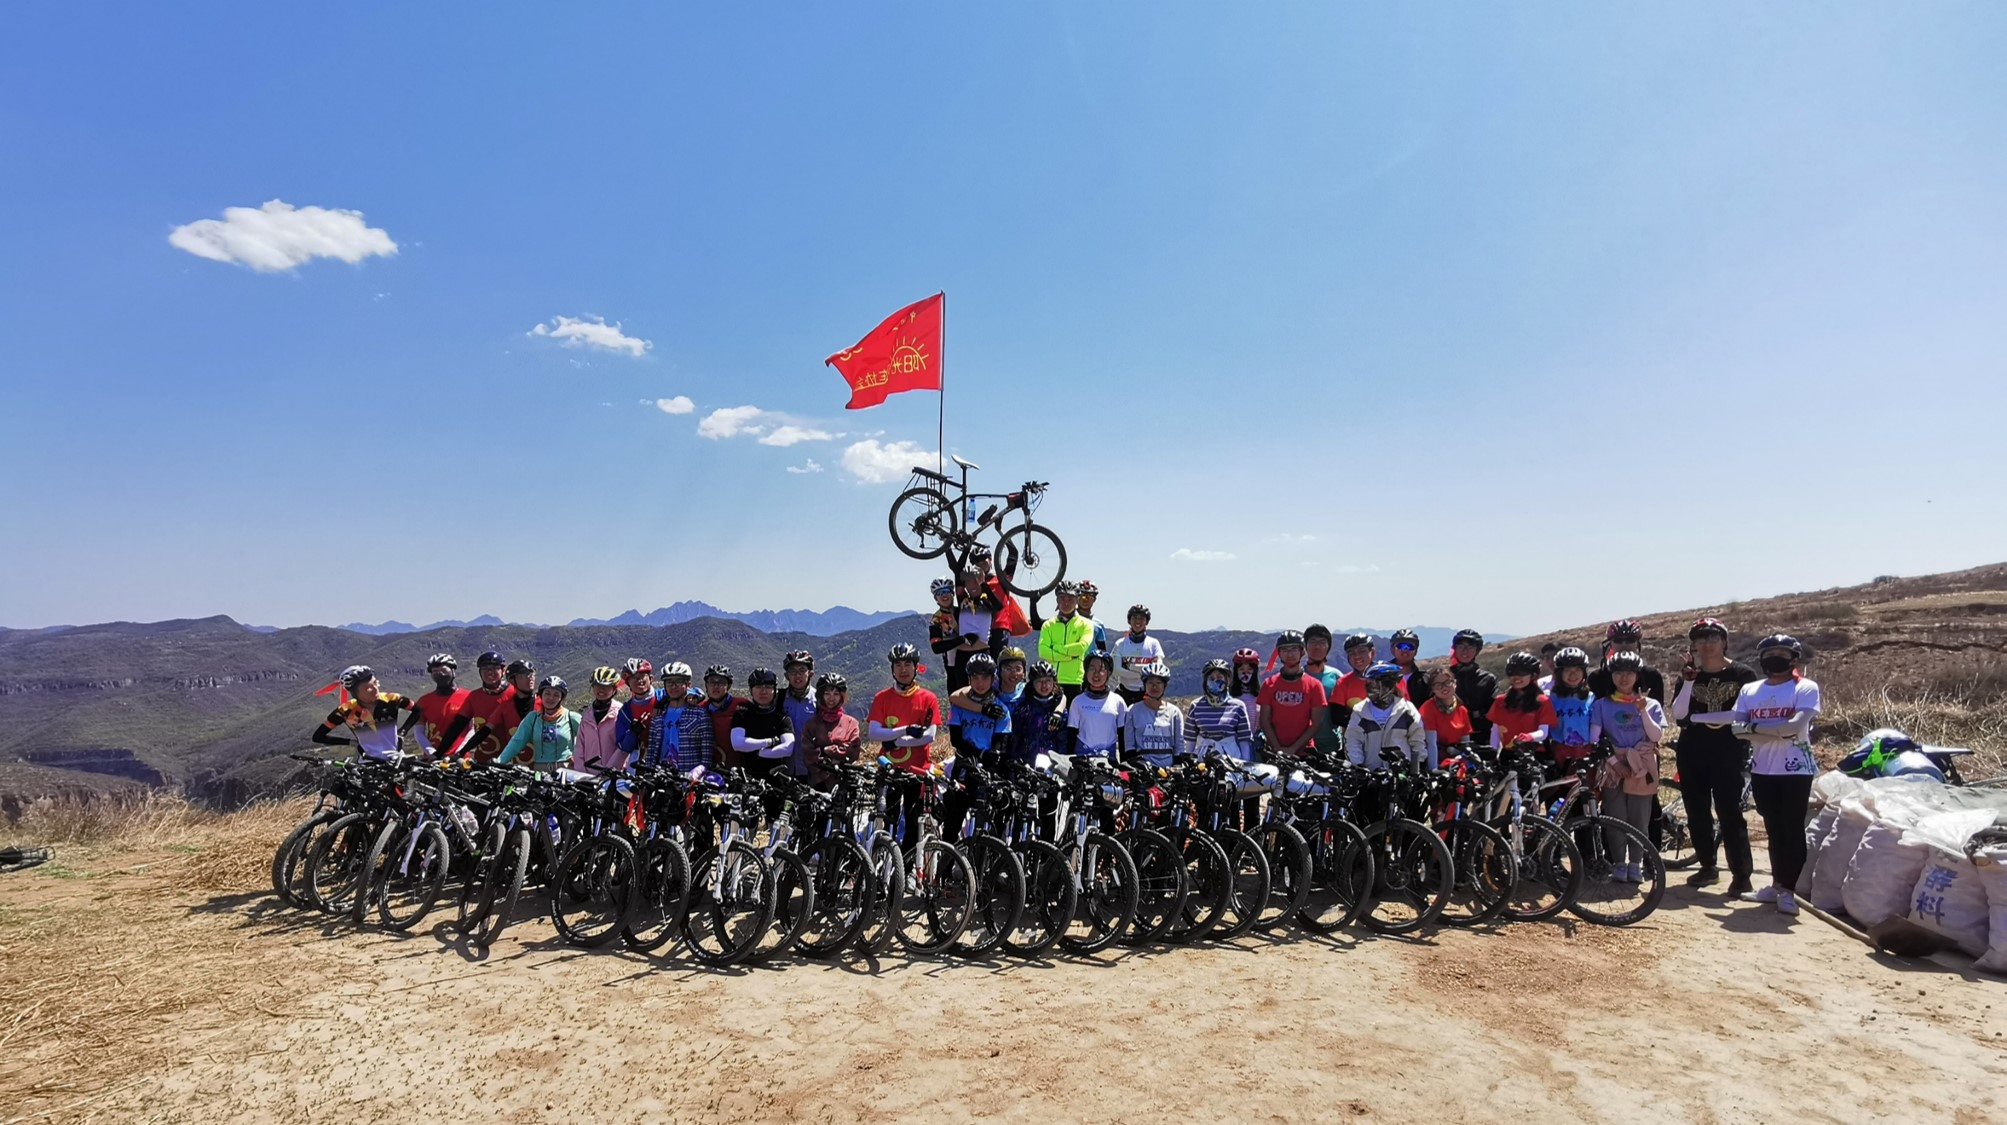
\includegraphics[width=0.3\linewidth]{fig/五一第二天.jpg}
    \hfill
    \caption{五一}
\end{figure}
\subsection{黑龙潭}
路书编号:2713774 返程2752063
\subsection{百里画廊}
路书编号:2713766
\subsection{幽州大峡谷}
路书编号:2604307,2605074

注意,第一天晚上应当到达幽州村,也就是要比去的时候的路书多骑几公里。



\begin{figure}[H]
    \centering
    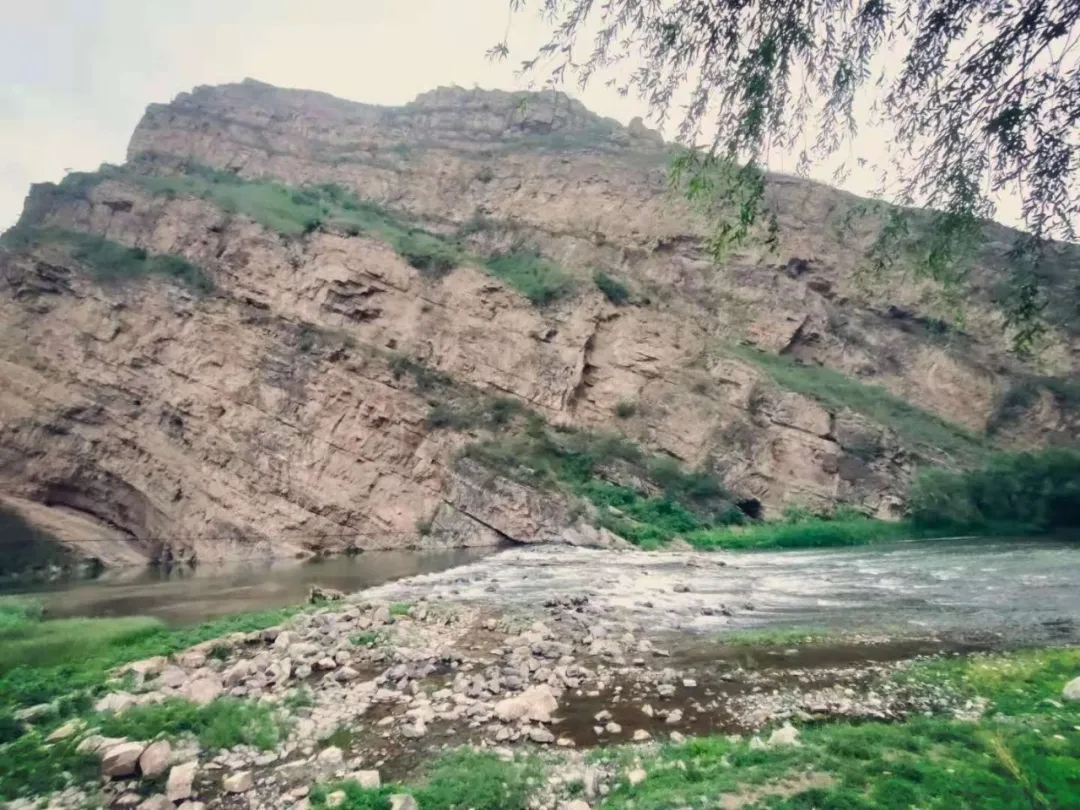
\includegraphics[width=0.45\linewidth]{fig/幽州大峡谷1}
    \hfill
    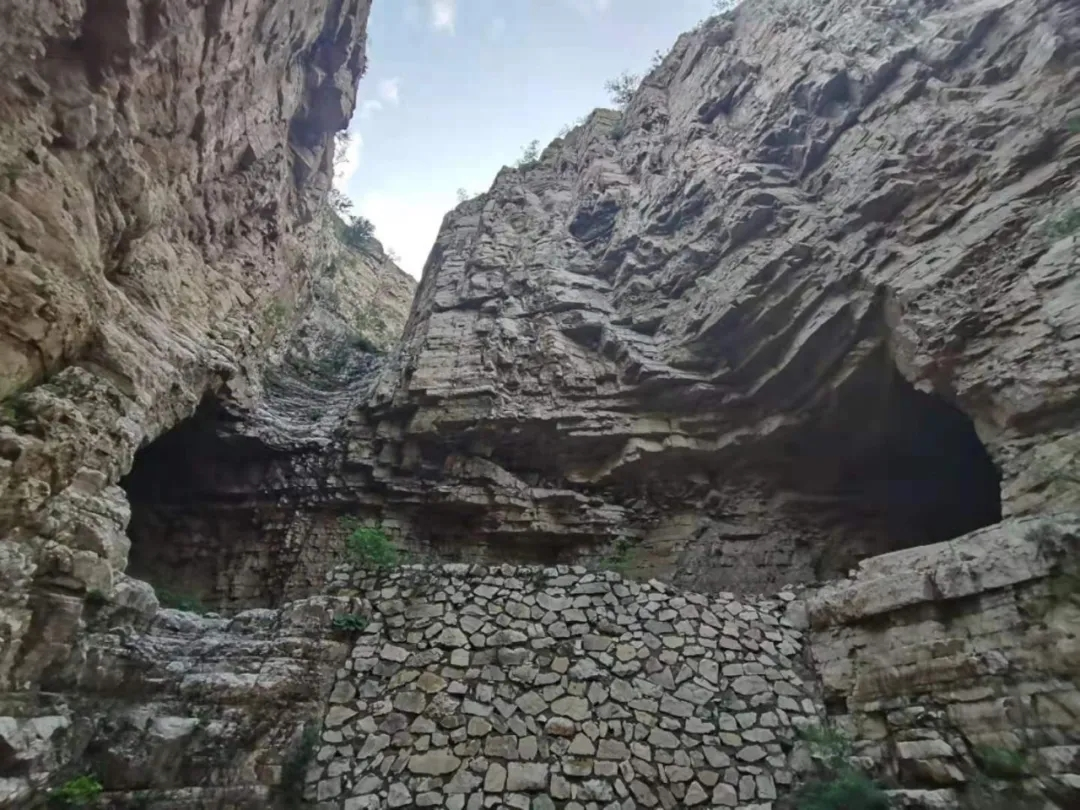
\includegraphics[width=0.45\linewidth]{fig/幽州大峡谷2}
    \caption{幽州大峡谷}
\end{figure}



\subsection{秦皇岛}
我说车协千万好,不如一次秦皇岛。
\begin{figure}[H]
    \centering
    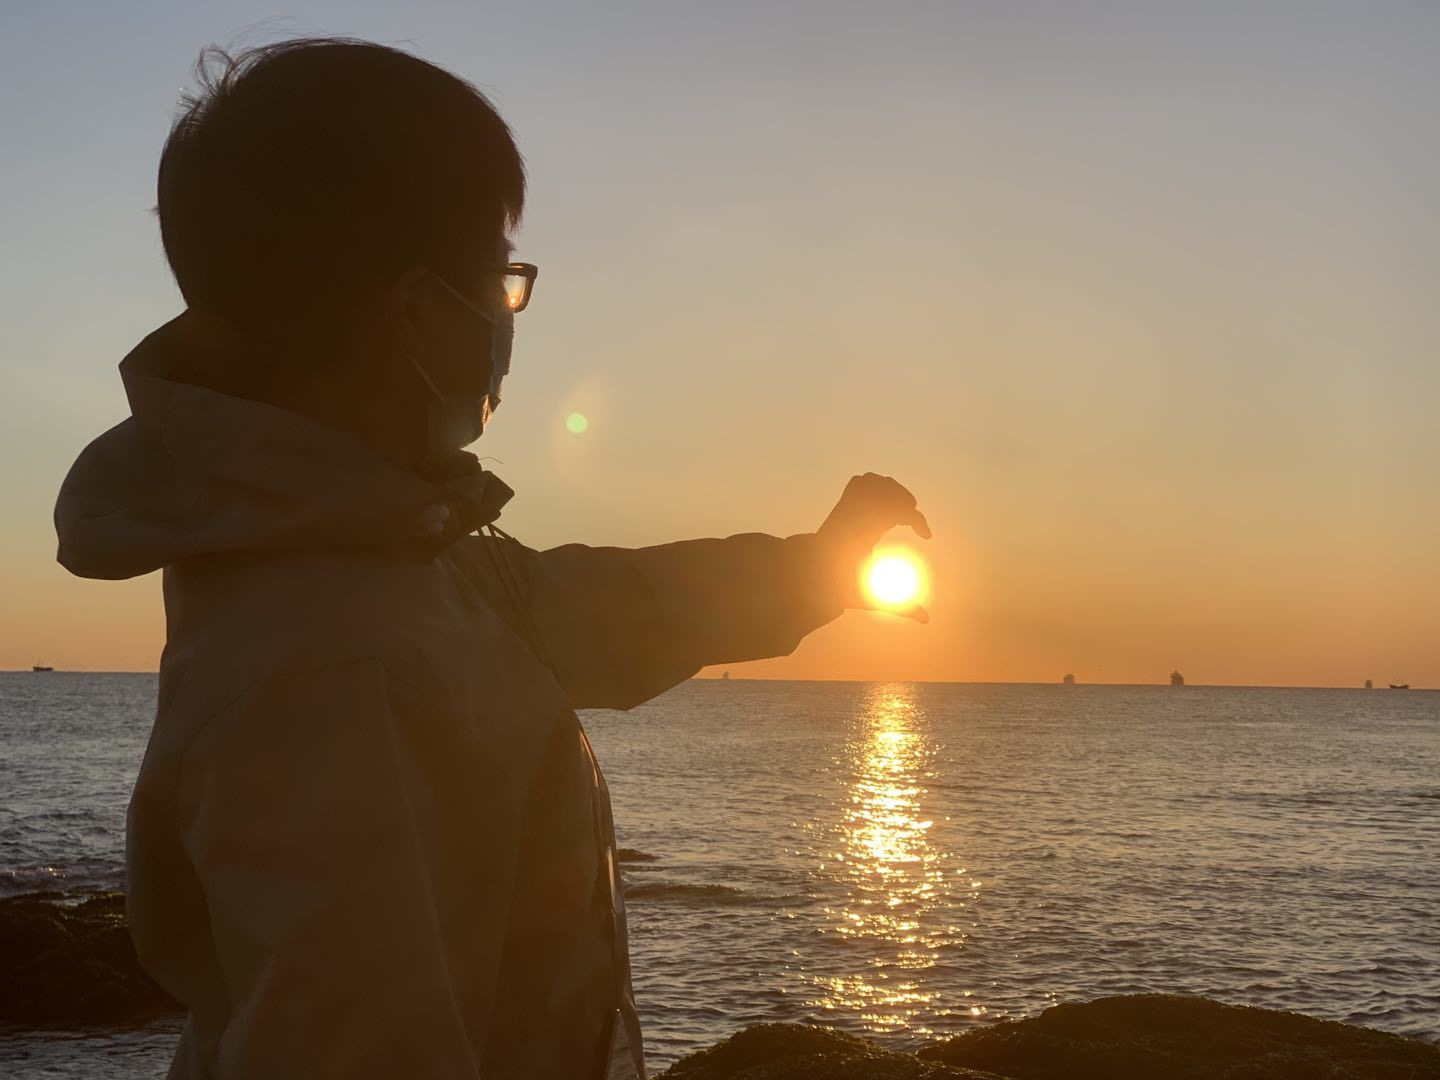
\includegraphics[width=0.45\linewidth]{fig/秦皇岛日出.jpg}
    \hfill
    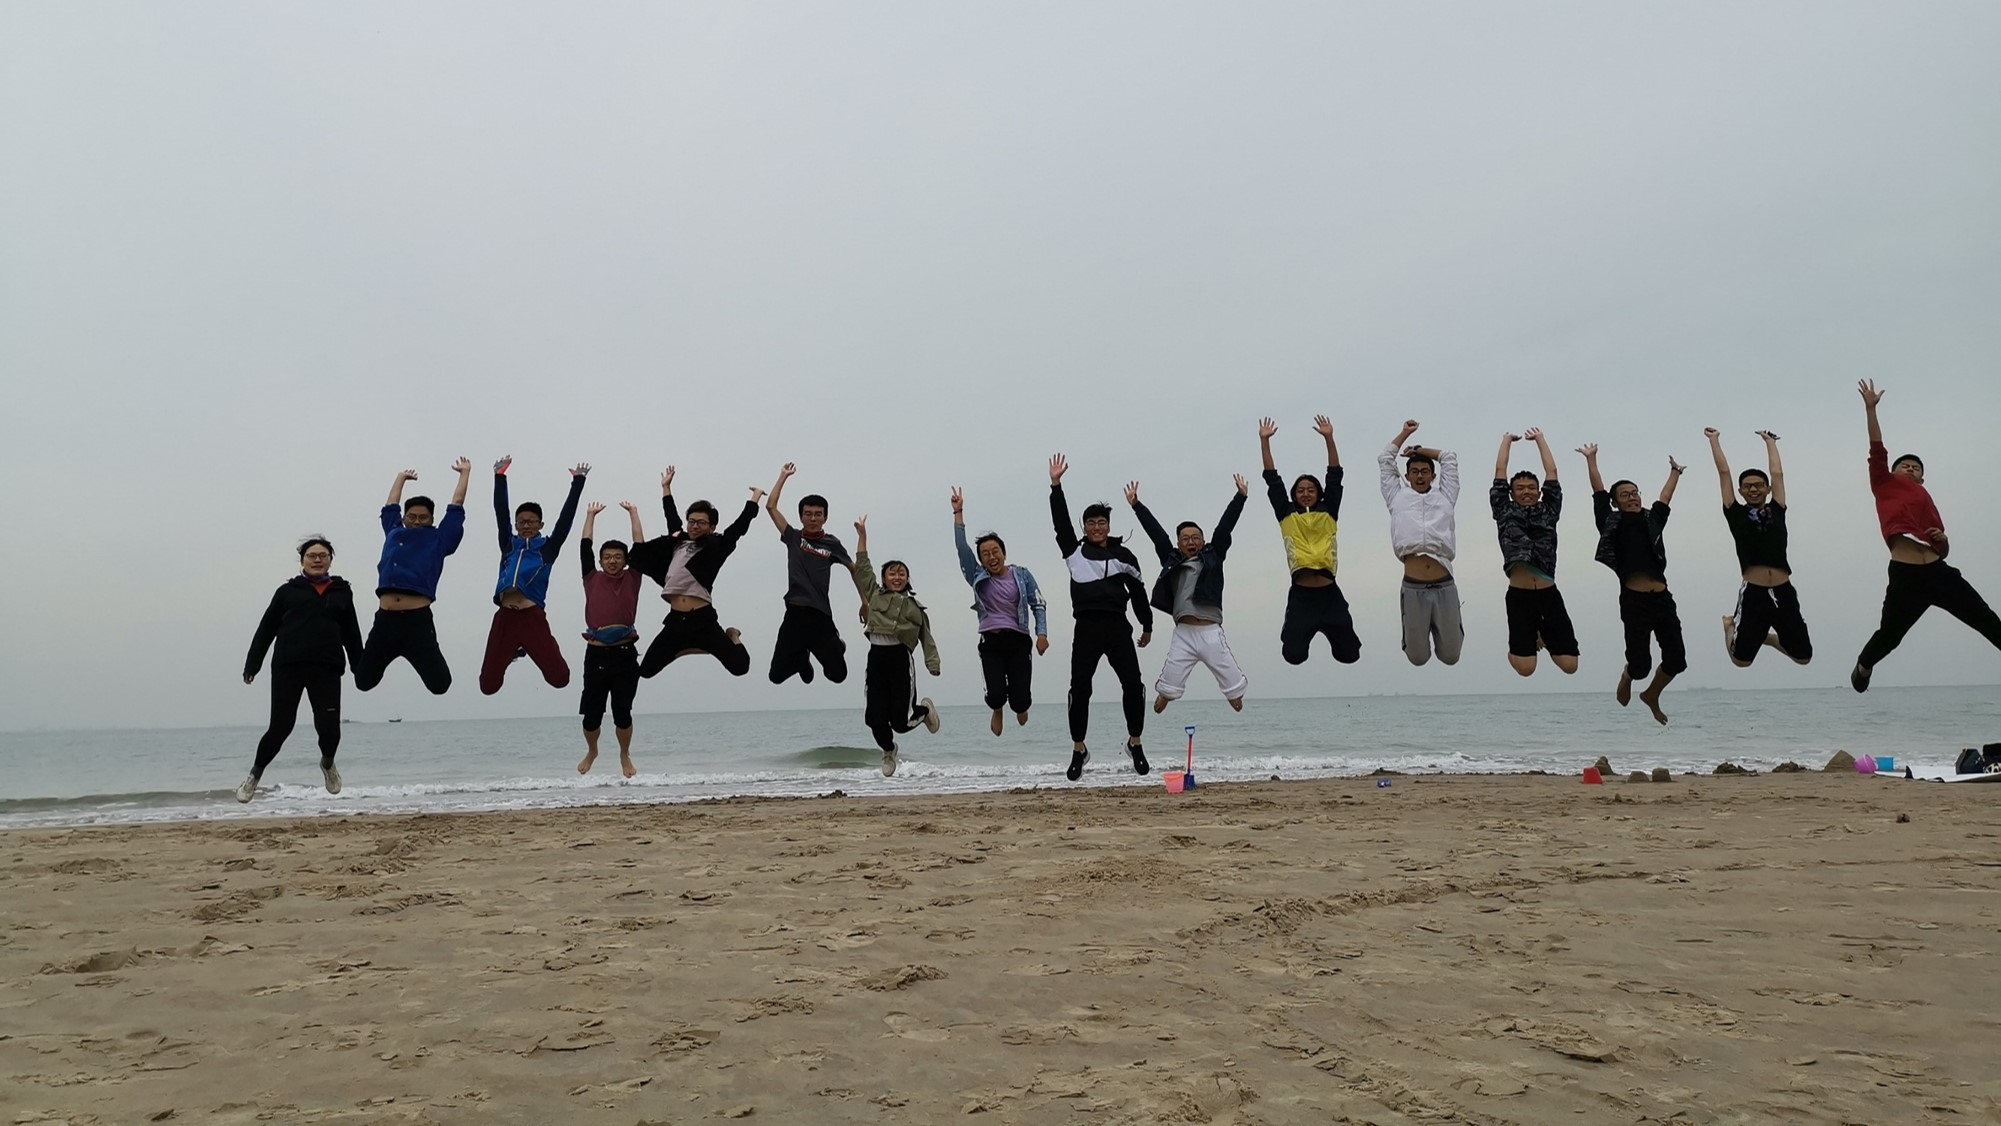
\includegraphics[width=0.45\linewidth]{fig/秦皇岛跳.jpg}
    \caption{秦皇岛}
\end{figure}

\subsubsection{预计费用}
2021年

总计 600 

第一天 晚饭、 住宿

第二天 午饭、 晚餐、 住宿

第三天 午饭、 晚餐、 住宿

第四天 住宿

第五天 聚餐,住宿

第六天 拖车、 大巴
\subsubsection{联系方式}
夏阿姨电话:13933569624
\subsubsection{日程安排}
\begin{itemize}
    \item 第一天
    
农大东区—河北省廊坊市华北科技学院(60km)

上午:进行安全培训,安全培训后分散吃午饭。

12点30准时从东区主楼出发。到达华科。
\item 第二天

上午:华科到天津市蓟县(50km) 中午在蓟县吃午饭

下午:蓟县到玉田县(34km)晚上进行团建游戏

\item 第三天

上午:玉田县-丰润区(40km)

下午:丰润区-卢龙县(69km)

\item 第四天

卢龙县-北戴河(60.5km)

午饭自由组队,不要一人出行。所在位置需及时于队长保持联系。

\item 第五天

早上可看日出

之后分三队:一队留在北戴河一队坐车去山海关;一队骑行去秦皇岛

\item 第六天

返程
\end{itemize}


\chapter{暑期远征}
\section{暑期选拔}
\subsection{暑期宣讲会}
宣讲会上一般要包括以下内容\notes{这里应当和前面的 {\textbf 室内活动——暑期宣讲会} 联系一起}
\begin{itemize}
    \item 路线公布
    \item 选拔方案公布
\end{itemize}
\subsection{队员选拔方案}
\begin{enumerate}[label={\chinese*、}]

\item 队员招募对象

身心健康,并注册成为阳光车协会员的所有人。
\item 选拔对象

具有被招募资格,在规定时间内报名并提交自述的所有人。
\item 预报名

注:报名表中所选择的队伍仅为预报名,最终报名队伍以暑期自述为准。
\item  选拔时间

4月9日-5月29日
\item 选拔内容
\begin{enumerate}
\item 积分

\item 体测

\item 团队评议

\end{enumerate}

\end{enumerate}

\subsection{预报名}
于4月15日23:00以前将报名表发至sunnybikefromcau@163.com,收到回复邮件后即为报名成功,逾期无效。报名表见附件。

邮件主题及报名表命名为''暑期报名+校区+姓名+性别``(如''暑期报名+东区+李琛+男``)

4月18日将在微信公众号上公布报名结果

注:报名表中所选择的队伍仅为预报名,最终报名队伍以暑期自述为准。
\subsection{暑期自述}
自述是一份必须要交的材料,内容包括:
\begin{itemize}
    \item 请注明自己选择哪支暑期队伍?(为了让更多的人体验到骑行的乐趣,我们增设了调剂选项,请你在自述中说明是否愿意接受调剂以及调剂意愿)
    \item 请简单做一个自我介绍。(说说自己的爱好,除了骑车跑步,比如特长、性格特点以及对大学生活的规划和愿景)
    \item 请列举自己在协会做过的事情或参加的活动,简单谈谈其中的收获和感想。
    \item 请认真做一个自我评价。说说自己在与人相处和待人接物上的优缺点,这些特点和能力在团队中将有怎样作用或影响,你将如何进一步完善和培养自己的能力为团队建设做贡献。
    \item 谈一谈你对自行车的认识和理解(自行车是一个怎么样的交通工具,骑行是一项怎么样的运动)
    \item 你为什么想去暑期(说说它最让你向往期待的部分),为暑期你即将做哪些准备。你最终报名哪支暑期队伍(同时请在自述开头注明),谈谈你对这支队伍的了解和期待;暑期路上你将为这支队伍付出什么,在队伍中担当怎样的角色,期望收获什么。
    \item 暑期回来之后你有什么打算,在后期的资料整理(图片、文字)、刊物编辑和未来的协会工作中你能做什么。
    \item 暑期路上,假如队长出现决策失误,给队伍行程造成了影响,你将如何应对以维护队长威信;假如某位队员出现了体力或情绪问题,你将如何帮他(她)化解情绪,融入团队。
    \item 报名实践队的会员,自述内容需额外说明:
    \begin{itemize}
        \item 谈谈对学校要求学生参加暑期实践的理解和认识;
        \item 通过自己对路线的了解,对在此路线上可开展的实践活动(或是可以发现的社会问题)发表自己的意见。
        \item 对实践队的活动形式、行程计划、人员分工等提出自己的意见、建议或者疑问,我们将在后期准备工作中充分参考大家的想法,把此次实践做得更好。 
字数不限,能表达清楚自己的想法就好。
    \end{itemize}
\end{itemize}
1、请务必在自述开头说明自己最终报名哪支远征队伍;自述中至少包含以上1—8点内容。
2、凡是报名暑期的会员必须提交合格的自述一份,如截止日期三天后仍未上交者,视为自动放弃暑期,取消选拔资格。
3、自述内容不会对外公开,只有理事会和队长可以看,作为评议时的参考,请大家务必认真对待。

自述上交时间:即日起至5月16日 23:00截止。

邮件主题命名为''最终报名队伍自述+校区+姓名+性别``如''骑行队自述+东区+蒋泽庆+男``

自述提交方式:发送电子版文档至暑期选拔公共邮箱sunnybikefromcau@163.com.

\subsection{暑期积分}

积分上限为40分,包括晚训及拉练两部分。

\begin{itemize}
    \item 晚训

 选拔期间,共16次晚训,每参加1次计1分

 要求无迟到无早退并完成规定训练内容,如发现迟到扣0.5分,早退扣0.5分,训练内容未完成扣0.5分,单次晚训分数扣完为止,不计负分。

\item 拉练

 共5次拉练,分别在第6、8、9、11、12周周末

 单日拉练计4分,五一小长途拉练计8分,总计24分

 5次拉练至少参加3次

\item 加分项
\begin{itemize}
    \item 晚训负责人加一分:本次积分过程中会选择3个固定的晚训负责人,积分期间分别负责带周一、三、五晚训,满4次即可加一分。
    \item  拉练活动队长加一分:每担任一次活动队长可加一分
    \item  秋季学期冬训队成队队员加一分
    \item  五一职务满贯加一分:在五一小长途活动中,担任队伍职务中的前骑、后骑及前站至少各一次,可加一分
\end{itemize}

\item 减分项
\begin{itemize}
    \item 活动迟到扣一分,当日活动队长及担任职务的队员迟到扣两分
\end{itemize} 

 

\item 积分及申诉要求

满25分者且参加过至少三次拉练者自动获得体测资格

不满足上述条件但拉练次数不少于两次且积分不少于20分者可向理事会提起申诉,经同意后获得体测资格。

注:若积分过程中出现特殊情况,及时向理事会反馈,会根据具体情况做出调整。

\item 申诉要求

申诉资格:拉练次数不少于两次且积分不少于20分。

内容要求:详细说明每一分没积到的原因,并谈谈自己对于暑期的看法。字数需在1000字左右。

\end{itemize}
\subsection{体测}

积分达到要求即可获取体测资格,包括跑步体测及爬坡体测两项。\notes{这里的体测应当和 {\textbf 日常活动-体测} 里联系起来。}
\begin{itemize}

\item 跑步体测:5月26日(周三)

男生:6000米(15圈),要求30分钟以内完成;

女生:4800米(12圈),要求28分钟以内完成。

\item 爬坡体测:5月29日(周六)

选取妙峰山经典爬坡路段\footnote{妙峰山路线详见 \pageref{subsec:妙峰山} 页}作为体测路段,全程约21km,累计爬升约900m。全体队员均由妙峰山山脚牌坊处出发

骑行队:

终点位于妙峰山山顶停车场(21km)

男生90分钟内完成,女生105分钟内完成

实践队和短途团:

男生终点位于妙峰山山顶停车场(21km),要求95分钟内完成;女生终点位于妙峰山山腰水站(14km),要求65分钟内完成。

\end{itemize}

\subsection{团队评议}

体测通过即可参加,包括参选队员互评及队长评测两项,各占50分。由参评队长及队员根据选拔期间个人观察以打分问卷形式打出。\notes{把团队评议的表格放到附录}

互评时间:5月29日晚(东区)
\subsection{积分及体测奖励}

积分:

 第一名:骑行驮包或音响

(以最后一次拉练结束后的积分排名为准)



体测:

第一名(男\&女):骑行驮包或音响

第二名(男\&女):组合

(体测名次为跑步和爬坡的综合排名)这是不是可以加个公式什么的
\section{成队事宜}
\begin{tips}
    成队前禁止建群。
\end{tips}
\notes{后面要在常见问题里写,为什么不能建群}


\begin{table}[H]
    \caption{个人/团队物资清单}
    \centering
    \begin{tabular}{|c|c|p{10cm}|}
    \hline
        \multirow{5}*{私人物品}
         & 衣物类 & 冲锋衣x1(带内胆),速干衣x2(队服+会服),运动鞋x1,拖鞋x1,一套平时逛街的休闲衣裤,短裤x1,长裤x1,薄外套x1,骑行服(选带),袖套,头巾,内衣若干,袜子若干,帽子(选带防晒用),雨衣 \\ \cline{2-3}
         & 装备类 & 骑行眼镜,头盔,手套x2(长指短指),车前灯,尾灯,手机支架,码表,护膝,管包,绑绳,防潮垫,驮包,备胎,魔术扣 \\ \cline{2-3}
         & 电子产品 & 手机,数据线,充电宝,音响,刮胡刀\\ \cline{2-3}
         & 日用品 & 牙刷,牙膏,毛巾,防晒霜,沐浴露,洗发水,水杯,笔,本,队记本,指甲刀,口罩 ,眼罩\\ \cline{2-3}
         & 其他 & 身份证,学生证,半价证明,现金,银行卡 \\ \hline
         \multirow{5}*{公共物品} & 装备类 & 补胎工具两套,打气筒x2,扳手x1,截链器x2,组合x4,润滑油x2,变速线x2,来令片x4,除锈剂x2,备胎x1(各型号),平嘴钳x1,镊子x1,记号笔x1,对讲机x3\\ \cline{2-3}
         & 日用类 & 电吹风x2,插排x2,针线盒,洗衣粉,垃圾袋,晾衣架,晾衣绳 \\ \cline{2-3}
         & 药物类 & 见队医物品清单 \\ \cline{2-3}
         & 宣传类 & 旗杆,队旗,会旗 \\ \cline{2-3}
         & 娱乐类 & UNO,狼人杀,扑克牌, \\ \hline
    \end{tabular}
\end{table}

\begin{table}[H]
    \centering
    \begin{tabular}{|c|c|c|c|}
    \hline
        基础物品: & 医疗物品: & 药品: & 队医包常备药品 \\ \hline
        一次性换药盘 & 创可贴 & 外用: & ~ \\ \hline
        一次性镊子 & 纱布敷料 & 云南白药喷雾(红+白) & 纱布敷料 \\ \hline
        一次性冰袋 & 无菌敷料 & 红霉素软膏 & 创可贴 \\ \hline
        一次性口罩 & 酒精湿巾 & 活络油 & 脱脂棉球 \\ \hline
        密封袋 & 卫生湿巾 & 花露水 & 碘伏棉球 \\ \hline
        小剪刀 & 脱脂棉球 & 云南白药(粉) & 换药盘 \\ \hline
        温度计 & 碘伏棉球 & 酒精湿巾 & ~ \\ \hline
        保温毯 & 碘伏棉签 & 内服: & ~ \\ \hline
        自粘弹性绷带 & 十滴水 & 碘伏棉签 & ~ \\ \hline
        生理盐水 & 仁丹 & 生理盐水 & ~ \\ \hline
        生理盐水 & 八味景天丸 & 绷带 & ~ \\ \hline
        普通棉签 & 红景天胶囊 & 十滴水 & ~ \\ \hline
        布洛芬 & 仁丹 & ~ & ~ \\ \hline
        维生素C & 金嗓子 & ~ & ~ \\ \hline
        葡萄糖口服液 & 西瓜霜 & ~ & ~ \\ \hline
        正露丸 & 纸巾 & ~ & ~ \\ \hline
        盐口服液 & 密封袋 & ~ & ~ \\ \hline
        金嗓子润喉片 & 镊子 & ~ & ~ \\ \hline
        西瓜霜润喉片 & ~ & ~ & ~ \\ \hline
        健胃消食片 & ~ & ~ & ~ \\ \hline
        仁和感冒药 & ~ & ~ & ~ \\ \hline
        999感冒灵 & ~ & ~ & ~ \\ \hline
        溃疡贴 & ~ & ~ & ~ \\ \hline
        枇杷露 & ~ & ~ & ~ \\ \hline
    \end{tabular}
    \caption{队医物品清单}
\end{table}


\subsection{运车}
需要带上身份证。
\subsubsection{中铁快运}
优点:
\begin{enumerate}
    \item 价格低廉
    \item 整车运输,不需要拆车
    \item 上门取件+送货上门
\end{enumerate}

缺点:
\begin{enumerate}
    \item 慢,平均时间为 4 到 5 天
    \item 略有暴力,可咨询当地站点可否打木箱
\end{enumerate}

价格:

打包费30元,运费依距离、重量而定。起步25kg,一般不会超过。

运车流程:

拨打电话 95572 告诉客服你需要运车,客服会很热情的帮你解决一切问题。服务态度好。

注意:运车的时候需要身份证,可能还需要提供购车发票,其实也就是证明你这个车是你的。这个东西看当地中铁的要求,有的要求的严,有的要求的不严。
\subsubsection{快递}
选顺丰或者德邦,千万不要选乱七八糟的快递。

优点:
\begin{enumerate}
    \item 快,2到3天,可以和自己的车多待几天
    \item 可以打木架,更加结实
\end{enumerate}

缺点:
\begin{enumerate}
    \item 相较中铁快运更贵
    \item 很多快递公司(特别是小地方的快递公司),没有运输这种大小的件的能力。
    \item 寄车就没有不暴力的
\end{enumerate}

价格:

运费依距离、重量而定。
\begin{table}[H]
    \centering
    \begin{tabular}{|c|c|c|c|}
    \hline
        车店 & 打包费  \\ \hline
        美利达 & 100  \\ \hline
        捷安特 & 100  \\ \hline
        德邦(纸箱) & 100  \\ \hline
        闪电 & 200  \\ \hline
        顺丰(整车,木架) &  300  \\ \hline
        德邦(木架/m³)  &  300  \\ \hline
    \end{tabular}
    \caption{北京地区运车参考价}
\end{table}

运车流程:

车店拆车打包,上门(车店)取件。

坚决抵制非专业的快递公司拆车打包,车店打包妥当,再寄出。

或:快递公司整车邮寄。
\subsubsection{物流}
物流比快递便宜,但往往有特定的线路,多打听找到联系方式。

优点:
\begin{enumerate}
    \item 便宜
    \item 可以车店直接发出,车店一般知道联系方式。
\end{enumerate}

缺点:
\begin{enumerate}
    \item 不方便,物流提供的是城市对城市的服务,也就是说到地方后要收货人去公司自提。
    \item 不确定性,物流时间往往不好预估。
\end{enumerate}
运车流程与快递相同。
\subsubsection{注意事项}
\begin{enumerate}
    \item 最好把上面码表这些小装备配件取下来,以免丢失。
    \item 最好用旧毛巾把车架,车把这些容易蹭的地方包起来,以免刮伤表面。
    \item 提前预估时间办理,以免人到了车还没到。
    \item 装自行车的纸箱两侧要有给搬运预留抓拿的地方。
    \item 封箱前请仔细检查拆下来的小配件有没装箱。
\end{enumerate}
\subsubsection{拆装技巧}
\begin{enumerate}
    \item 打包前先把后拔变速到最大飞上,前拔挂到最小盘上,让后拔尽量微里靠,找东西挡住后拔变速器进行保护。
    \item 把水壶架拆了,前轮碟片这一面朝里,让碟片躲在车架三角架中间,用扎带固定好不让前轮窜动。另一侧用车行打包的塑料保护件盖好。
    \item 前轮快拆杆是必须要拆下来的。
       \begin{figure}[H]
            \begin{center}
            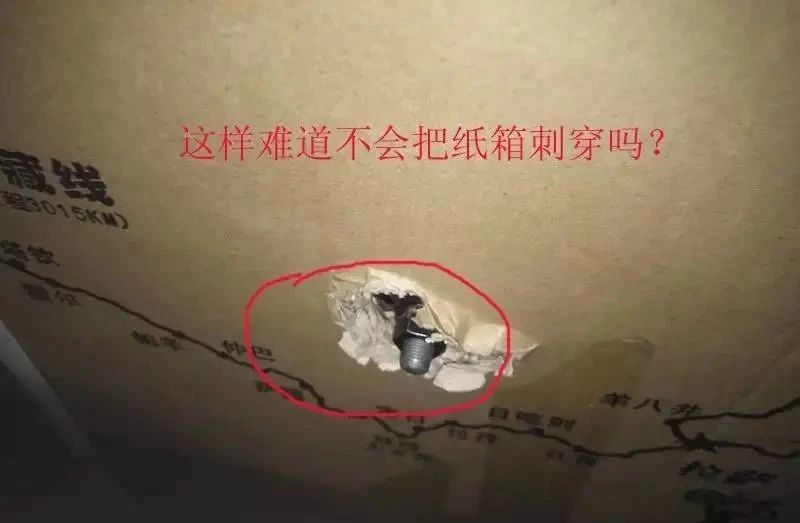
\includegraphics[width=0.6\textwidth]{fig/快拆杆}
            \end{center}
        \end{figure}
    \item 油碟前轮拆了之后,必须在来令片之间塞一塑料片,用硬的纸板也可以,以避免刹车把无意压住后左右来令片合在一起,此时绝对不可以去捏刹车把。
    \item 车把的拆卸。
    \notes{这里改成并排放两张,不然太占空间了}
       \begin{figure}[H]
            \begin{center}
            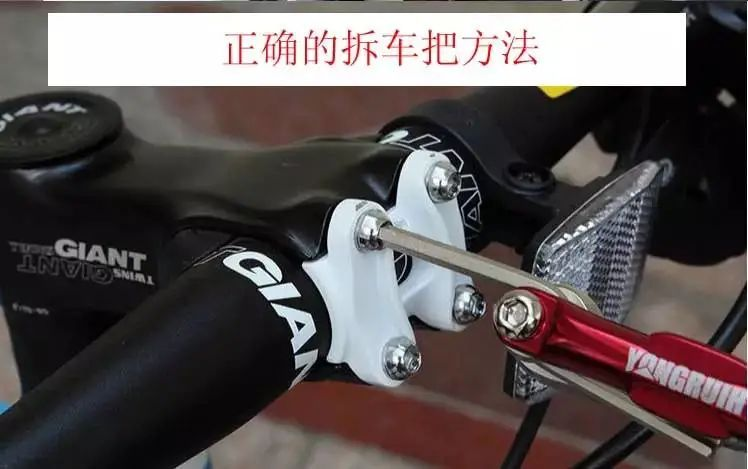
\includegraphics[width=0.6\textwidth]{fig/拆车把1}
            \end{center}
        \end{figure}
       \begin{figure}[H]
            \begin{center}
            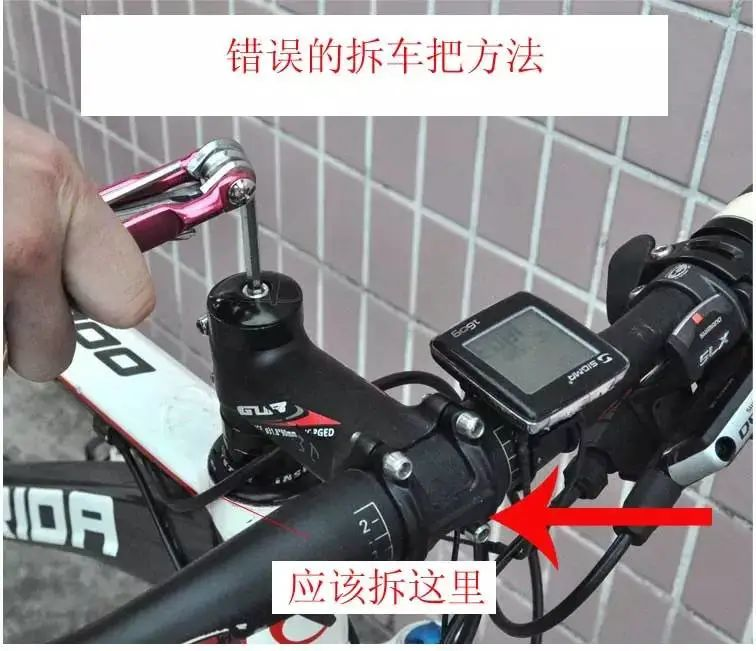
\includegraphics[width=0.6\textwidth]{fig/拆车把2}
            \end{center}
        \end{figure}
    \item 车把、前叉安装注意正反。
    \item 脚踏安装不好,整套牙盘报废。安装脚踏经常出现的问题有两点:左右与松紧。

一般是用15的开口扳手。

脚踏上面一般都有标记L、R。

必须用手去对正旋转进去,差不多了才用工具稍用力紧下即可。严禁最开始就用工具去安装,一但有点歪工具用力拧进去就会把曲柄的螺纹损坏。

踏板太松会将曲柄的螺纹孔摇滑丝。滑丝之后,你得更换整套牙盘,除非你上淘宝网购单边损坏配件!

\end{enumerate}
\section{暑期远征}
\subsection{车票}
无非就三种选择:飞机,火车,大巴

一般来讲,我们推荐火车硬座。

如果是正常买票的话,跟我们平时出行没什么区别,此处不再赘述。\notes{学生票购买方法}

\begin{tips}
    硬座是车协传统,在硬座可安全到达的情况下,优先硬座,情怀在。
\end{tips}
\notes{没说清楚这个硬座的意义}
\subsection{高原骑行注意事项}
1,防高反的重点是防感冒;

2,防感冒的重点是及时加减衣物;

3,晚上睡觉窗户不要关闭太严;

4,晚上睡觉床边备好饮用水;

5,高海拔地区不要大吼大叫,不要猛烈跳跃,久蹲不要突然站;

6,贴身必须穿速干面料衣服;

7,保暖层衣服必须拉链式,便于打开散热,便于穿脱;

8,放坡前必须做好保暖措施,分体雨衣一半的作用是下坡防风;

9,放坡头部保暖是重中之中;

10,路上要喝热水,一定要有保温水壶;

11,感冒了建议坐车去低海拔站点休整,感冒状态建议不要洗澡;

12,身体不适及时就医,高原不要硬撑,你撑不过的;

13,高海拔地区不要饮酒,更不能酒后洗澡;

14,体力不好的不要硬跟体力好的,按自己节奏安排行程;

15,高原骑行,买东西可以节约,但请别在吃上省钱,不吃哪有力气骑车,不吃身体哪有抵抗疾病的能力,多吃水果(苹果、香蕉、梨等);

16,长时间放坡要间歇停下休息;

17,下坡不要紧跟大货车,队友间保持安全距离,不要占道超车,不要夜骑;

18,经过塌方、落石地段多观察,确认安全情况下快速通过;

19,休息地选择宽阔地带,不要靠近山体、悬崖、河边;

20,不要去撩流浪狗,流浪猫、土拔鼠等动物,你爱它,它不一定爱你!

21,新手不要站起来摇车,陡坡不要强撸,膝盖保暖护膝必备;

22,睡觉前请给家人报个平安,不要关机睡觉;

23,紧急情况,就近拦车求助,并及时拔打110或120;

24,如遇客栈停电发电时,请不要充电,以防电压不稳定烧毁;

25,出发前请为自己购买一份户外保险;

26,高原骑行,适时休整,劳逸结合,过度劳累可能会引发其他疾病。

\subsection{一些经验}
\notes{这里说的太笼统了,要对每一句话做解释。}
\begin{itemize}
\item 气象人可以抓来看风向
\item 不要相信你的巧克力
\item 不要带电脑(不听老人言,吃亏在眼前)
\item 对讲机很有用,建议一个队三个(真好用)
\item 除锈剂那些液体没有盖的别带了
\item 磨砂洗手液好用的一批
\item 建议队伍里多搞大防潮垫(单人防潮垫没怎么用过),买厚的
\item 北方路线可以洗澡堂,住不能洗澡的宾馆,便宜
\item 住网吧包夜
\item 吃不完的干粮带走,馒头花卷什么的
\item 脚撑好好买
\item 终点设置在一个阳间点的地方
\item 带一个可以装随身物品的小包
\item 打木架可以找木匠
\item 补好的胎装进盒子里或用扎带扎好,没补好的裸着,做好区分
\item 出发前检查老车,外胎、变速、链条、刹车……
\item 打木架可以找木匠
\item 找不到地方寄车的时候问一问当地人,比如电动车店
\item 去冷/湿的地方带保暖救生毯
\item 免胶补胎片片很好用
\item 后骑带吃的,但不要放进后骑包里
\item 关注途径点的公众号,随时关注道路及防疫信息
\item 不要随便相信陌生人,他不用对你负责,遇事多打听
\item 不要相信阴间黑暗快递,最起码要有单号
\end{itemize}
\section{暑期后}
\subsection{视频剪辑}
\subsection{暑期报告会}
\chapter{常见小游戏}
小游戏主要是在大家休息的时候,为了防止冷场而设立的
\notes{这里太乱啦,把小游戏整理整理}
\section{室内小游戏}
这里的小游戏主要是用于生日会和新生见面会。用于热闹氛围的。

注意,大多数情况下,很难让所有人都参与游戏,只能有几个人参与游戏。因此,游戏要有观赏性,让台下的人也觉得很有趣,而不是只让台上的玩好。

\section{室外游戏}
这里的游戏主要用于校庆嘉年华,五四嘉年华,拉练中的休息时间。

\section{狼人杀}
\section{麻将}
\section{三国杀}
\section{扑克}
\section{竞慢}
\section{轮胎放气}
\section{小姐牌}

玩此游戏首先需要找到一副或一堆散牌,剔除大王和小王。要有人负责发牌,一人发一张,一个一个人的轮着发,发一张看牌是啥,玩对应的小游戏,小游戏结束,再给下一人发牌。


游戏牌介绍:

A:命令牌。

得到此牌的人,可以命令参与游戏的任何一人喝一杯酒。

小游戏结束,此牌失效。

2:小姐牌。

得到此牌的人,需要大声喊:''我是小姐!``,充当小姐。

当别人输酒时,别人可以喊:''小姐何在?``这时,小姐必须回应:''小姐在此,大哥吃好喝好。``并且要跟着喝一杯酒!

下一小姐牌出现,上一小姐牌失效。

注意:和气最重要,如果遇女士得到此牌不好意思,可以跳过切勿强求。

3:星期天游戏。

从得到此牌的人开始喊:星期天。

下个人喊:逛公园。

再下个人喊:逛的啥。

再下个人喊:天上飞的/地上跑的/水里游的。(注意是3选1!!)

挑战在这里,之后的人接着喊对应的动物名。如上个人喊天上飞的,这时就必须喊麻雀、乌鸦等。必须是2个字的,且不能跟人重复,还不能包含老、大、小!老鹰、大雁、都算输。

输的人喝酒。小游戏结束,此牌失效。



4:自由pk游戏。

得到此牌的人,可以指定1人跟他PK游戏。共同商量玩法,玩啥都行,猜媒、猜有无等。输的人喝酒。

5:照相机。

得到此牌的人,只要叫''照相机``,全桌的人不许动,保持静止3-5秒。谁动罚酒一杯。没人动,自罚一杯。(5照相机有效时间和2小姐牌一样)

使用后失效,未使用下一张出现自罚一杯后失效。

6:几棵柳树扭几扭。

依次向下顺着说,几棵柳树扭几扭。(举例说:拿到6的人可以说''3棵柳树扭3扭``,那么下一个人就说''4棵柳树扭4扭``),依次继续,谁输谁喝一杯。

小游戏结束,此牌失效。



7:逢7过。

就玩逢7过的游戏。(就是那个7、17、27................以及7倍数喊过的游戏)。

8:尿片牌。

只有拿到8才能上厕所,没有8去厕所必须喝酒。

9:自罚一杯。

10:神经病牌。

得到此牌的人,先喊:''我是神经病``。

之后,此人说任何话,你都不能搭理他。谁搭理他谁输酒。

有人中招后失效,未有人中招时下一张出现自罚一杯后失效。



J:左边喝。

得到此牌的人得左边的人喝。

Q:右边喝。

得到此牌的人的右边的人喝。

K:定量。

首次出现,得到的人喝一杯。喝后规定下一个拿到K的人喝多少,那个人就得喝多少。
\section{炸金花}
\subsection{游戏规则}
游戏人数可为2―4人,使用一副扑克牌,去掉大小王,共52张牌。游戏开始后,玩家先将底注投入,从庄家开始逆时针顺序每人发三张暗牌,第一次开局随机选择庄家。用户可以通过''看牌``或者猜测对方牌来进行''下注``、''跟注``或者''放弃``,最后剩下来的2个人,则可以随时开牌,或者玩家数大于2人以上,但是已有玩家选择''封顶``时,则由系统开牌,并根据比较规则来判断胜负。

封顶:本次下注后,其他玩家跟注后必须开牌。

\subsection{牌型说明}
\begin{itemize}
\item 豹子:三张同样大小的牌。
\item 顺金:花色相同的相连三张牌。
\item 金花:三张花色相同的牌。
\item 顺子:三张花色不全相同的相连三张牌。
\item 对子:三张牌中有两张点数同样大小的牌。
\item 单张:除以上牌型的牌。
\end{itemize}
\subsection{牌型比较}
\begin{itemize}
    \item 豹子 >顺金 >金花 >顺子>对子>单张;
    \item 顺金、顺子按照顺序比点。AKQ >A23>KQJ>...234;
    \item 单牌大小比较:A>K>Q…..>2。
    \item 对子大小比较:先比对,对同等大再比单牌;
    \item 比牌牌型等大,先开为负。
\end{itemize}






\section{贴贴}

偶数个人,其中一个人抓,另一个人跑。其余的人两两一组。跑的那个人可以贴到别的组上,然后那个组的另一个人就得跑。

\newpage

\chapter{骑行装备}
\section{人身装备} 
    \begin{itemize}
        \item 头盔
    
        头盔对骑行者的重要意义不言而喻,不带头盔者严禁上路。\notes{这里的每一个装备都应当有照片}
    
        检查头盔是否有裂痕或其他明显损坏
    
        头盔前沿与眉部平齐而不遮挡视线
    
        捋顺并收紧束带至头盔不能自由移动,与头部贴合完好并左右对称。
\begin{figure}[htp]
    \centering
    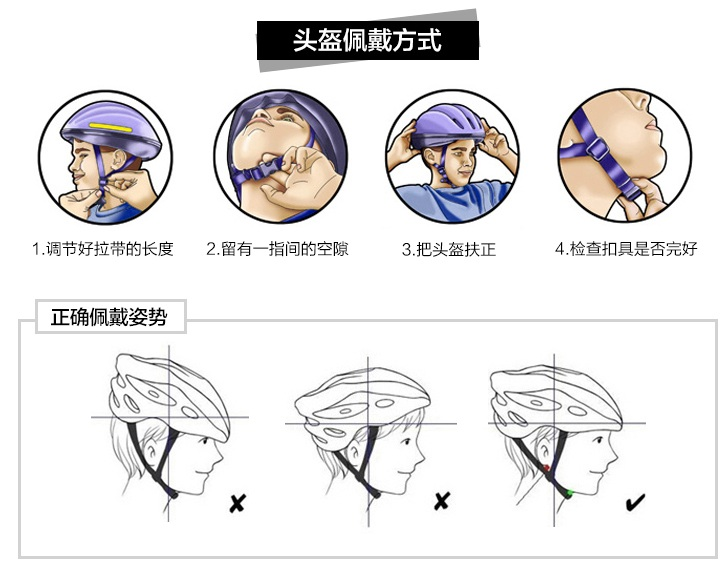
\includegraphics[width=0.7\linewidth]{fig/头盔佩戴方法.jpg}
    \caption{头盔佩戴方法}
\end{figure}

        \item 绑腿
        
        如果裤腿太宽松的话,有可能会被卷进链条,绑腿可以绑紧裤腿,避免发生意外。
        \item 暖足贴
        
        冬天骑车,最冷的就是脚指头,简直要冷到骨子里了。强推暖足贴。
        \item 手套    
    
        平常骑行的过程中可以起到有效的缓冲作用,在摔车时,可以为你的手提供一层防护。
    

        \item 头巾  
        
        头巾不仅仅可以防止你被晒黑。更重要的是它可以避免你的脸被晒伤,被风吹到干裂
    
        头巾有很多种用法,可以裹在脖子上和脸上,防止晒伤。还可以绑在额头,防止汗水低落在眼睛上影响视野。
    
        可保护脸部不被晒伤,还可挡风遮尘。有的车友把头巾直接罩在头上,头巾中间开两个洞露出眼睛,算是比较另类而实用的使用方式。另外还可以在头盔内衬一条头巾,能够吸收额头上的大量汗水,避免汗液滴到眼睛里影响视线。

        \item 冰袖
    
        也叫袖套,是用尼龙或涤纶与氨纶或莱卡面料混合制成,通风与速干性能较好,套在手臂上能起到一定的防晒作用,甚至会起到降温的作用。

        \begin{figure}[H]
            \caption{啄木鸟冰袖}
            \begin{center}
            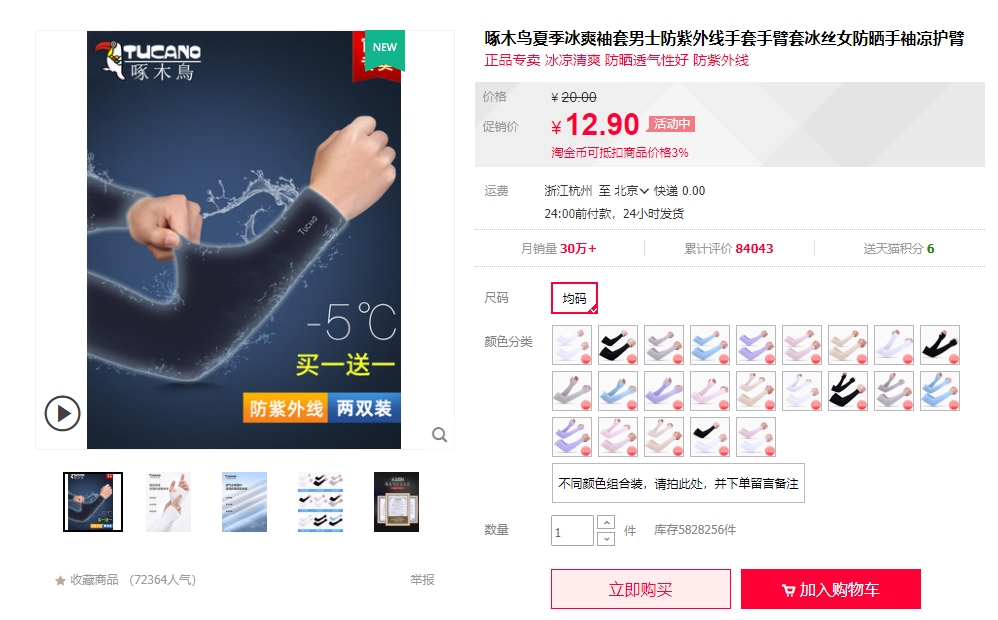
\includegraphics[scale=0.3]{fig/啄木鸟冰袖.png}
            \end{center}
        \end{figure}

        价格大约在10元到20元一双,不用买太贵的,意义不大。
        \item 骑行眼镜
        \item 骑行服

    \end{itemize}
    
    \begin{itemize}    
        \item    冬季穿衣技巧
    
    首先说一些常识

不要穿纯棉的衣服,出汗往身上一贴冷的一比\notes{不要把穿衣技巧放到装备里啊。。。放到附录也比这里合适。成队前禁止建群。}

骑起来的时候下肢比上身和手脚抗冻,停下来就没区别了

出门前看天气,善用彩云或者windy等app,了解山区和城区的温度差异

刮风4级以上,体感温度-5度

最好不要玩命骑出一身汗,然后放长坡

北京最冷的月份是12月下旬到1月上旬,一般过完年就开始暖和了

冬天常规的骑行服分三种功能,排汗、保暖、防风:
排汗一般为速干材质,贴身穿着,协助透气及排出水分,不会像纯棉材料吸水裹在身上

保暖一般为抓绒材质,在排汗外穿着,防止冷空气入侵,锁住热量

抓绒材料在大风和放坡的时候无法阻挡冷风侵入,此时就需要防风衣物了

以上三种材料不一定单独出现,有些产品会包含其中两种属性,大部分骑行服品牌都有自己的冬装,购买的时候首先要看自己的需求和衣服材料是否对应,其次看产品说明适应的温度,适应温度越低的一般就越厚越保暖。

不同温度下的推荐穿着(只对应北京气候,南方的魔法攻击不在参考范围,本人怕冷,比较抗冻的可以在此基础上减一层):
10-15℃,上衣排汗+薄长袖骑行服,下身抓绒短裤

5-10℃,上衣排汗+抓绒长袖骑行服,下身抓绒长裤,薄长指手套

0-5℃,上衣排汗+抓绒防风(软壳)骑行外套,下身防风抓绒长裤,厚长指手套,戴鞋套

-10-0℃,上衣抓绒排汗+马甲+抓绒防风(软壳)骑行外套,下身骑行秋裤+防风抓绒长裤,医用一次性手套+厚手套,两双袜子中间裹一层锡纸,戴鞋套,大耳罩子

-10℃以下,台子不香吗?


有一个很简单的看自己穿的衣服合适不合适的方法,骑车当天穿好衣服站在外面,如果觉得冷,但不是冷的受不了的那种,那基本是合适当天骑车的穿着。如果觉得很舒服,不冷不热的,那就是穿多了,骑起来一定热,要么边骑边脱衣服,要么出一身汗以后停下来变的更冷。
\end{itemize}
    
\section{车身装备} 
    \begin{itemize}
        \item 外胎
        
        如果是单纯骑铺装路的话,可以考虑把普通的山地车外胎换成光头胎,速度会更快。带来的问题就是会导致车辆的通过性更差。

        \item 内胎
        
        注意:长途中应当多准备26寸法嘴的内胎,因为26寸法嘴的内胎可以装在:26寸法嘴,26寸美嘴,27.5法嘴,27.5美嘴的轮组中。\footnote{如果对此条感到疑问,可以自行尝试一下}同样,27.5法嘴的内胎也可以装在27.5法嘴,27.5美嘴,29法嘴,29美嘴的车中。如果觉得法嘴的内胎装在美嘴的车中不稳,可以向车店讨要用于固定法嘴的小零件。(或提前自行上网购买,关键词:美嘴转法嘴固定座)
        
        \item 车锁
        
        像下图这样的车锁基本不用考虑了,因为它的可靠性很差。即使没什么工具,两块石头三两下也砸开了。真$\cdot$防君子不防小人

        但是你钥匙丢了就很方便了,dddd.

        \begin{figure}[H]
            \begin{center}
            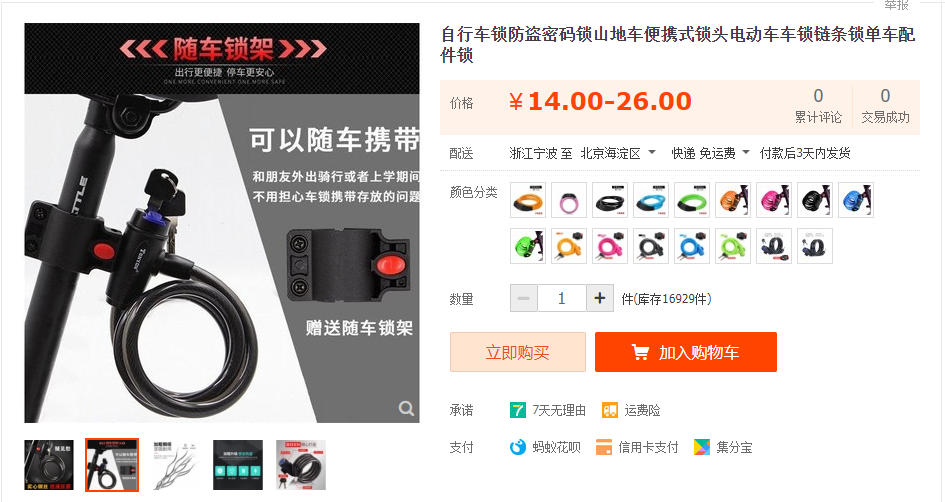
\includegraphics[scale=0.3]{fig/劣质车锁.png}
            \caption{劣质车锁}
            \end{center}            
        \end{figure}

        建议买100元起步的可以放在车上的折叠锁,比较方便,美观,结实。另外,既然选择了带锁,就一定要把钥匙带上!!!

        \begin{figure}[H]
            \centering
            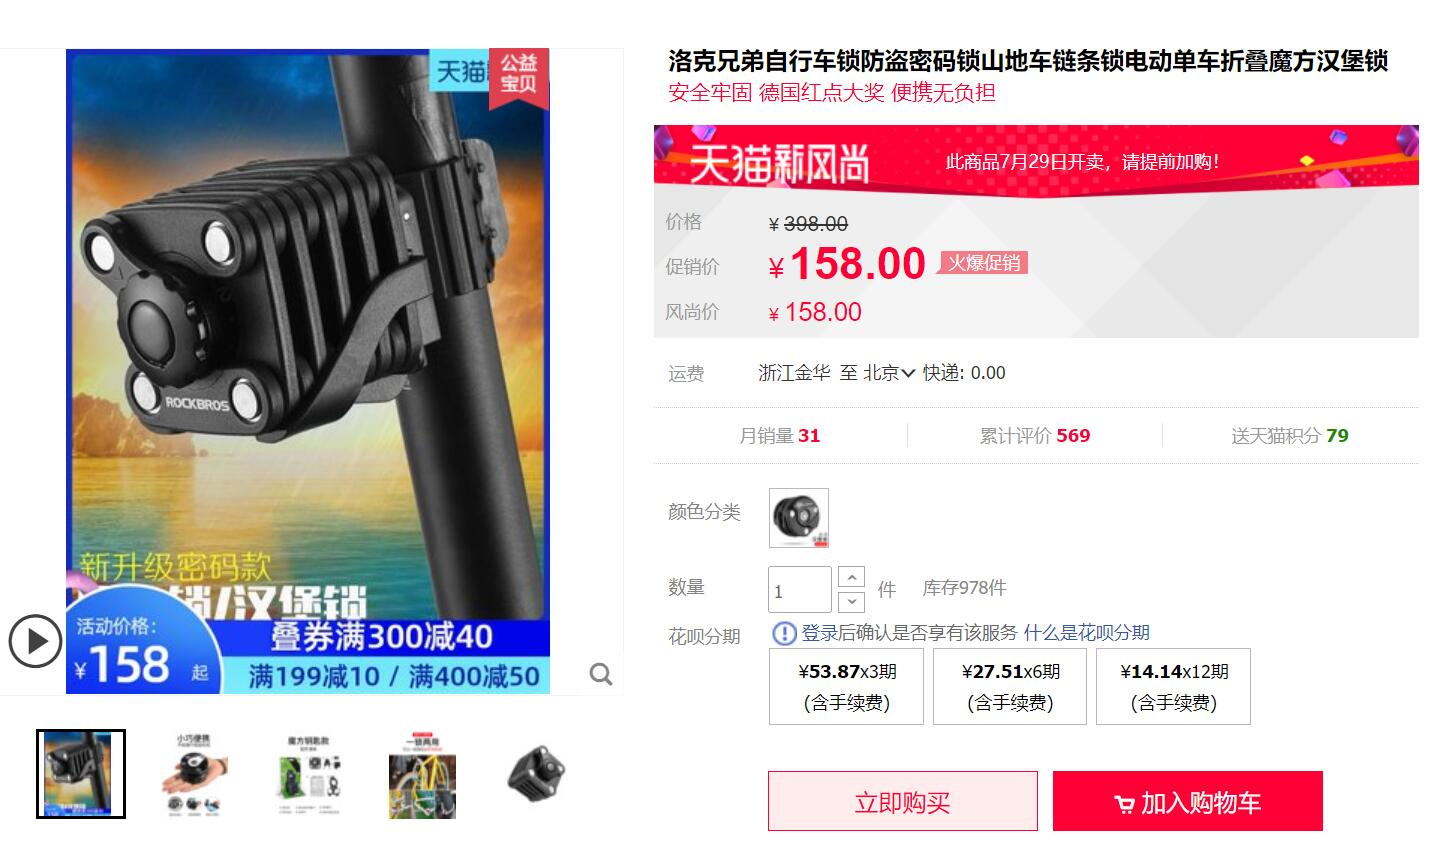
\includegraphics[width=0.7\linewidth]{fig/魔方锁}
            \caption{魔方锁}
        \end{figure}
        

        \item 码表
    
        码表的差距非常大,根据你的需求不同,价格也就不同。淘宝上便宜的码表只有19元,而贵的码表可以贵到两三千。
        
        如果只是想简单的记录一下数据,看看自己哪年哪月哪日骑过什么什么路,那就看你平时用的骑行软件适配什么码表,就买什么码表。比如行者的 ''小G``

        如果不是想搞竞速需要专业训练的话,行者的''小G``足够满足需要了。''小G``可以提供时速,最高速度,平均速度,坡度,累计骑行距离。更好的是,它可以记录你的骑行轨迹和数据保存在码表中,在你有空的时候,可以通过蓝牙来把码表中的数据导入到你的行者APP中。

        \begin{figure}[H]
            \centering
            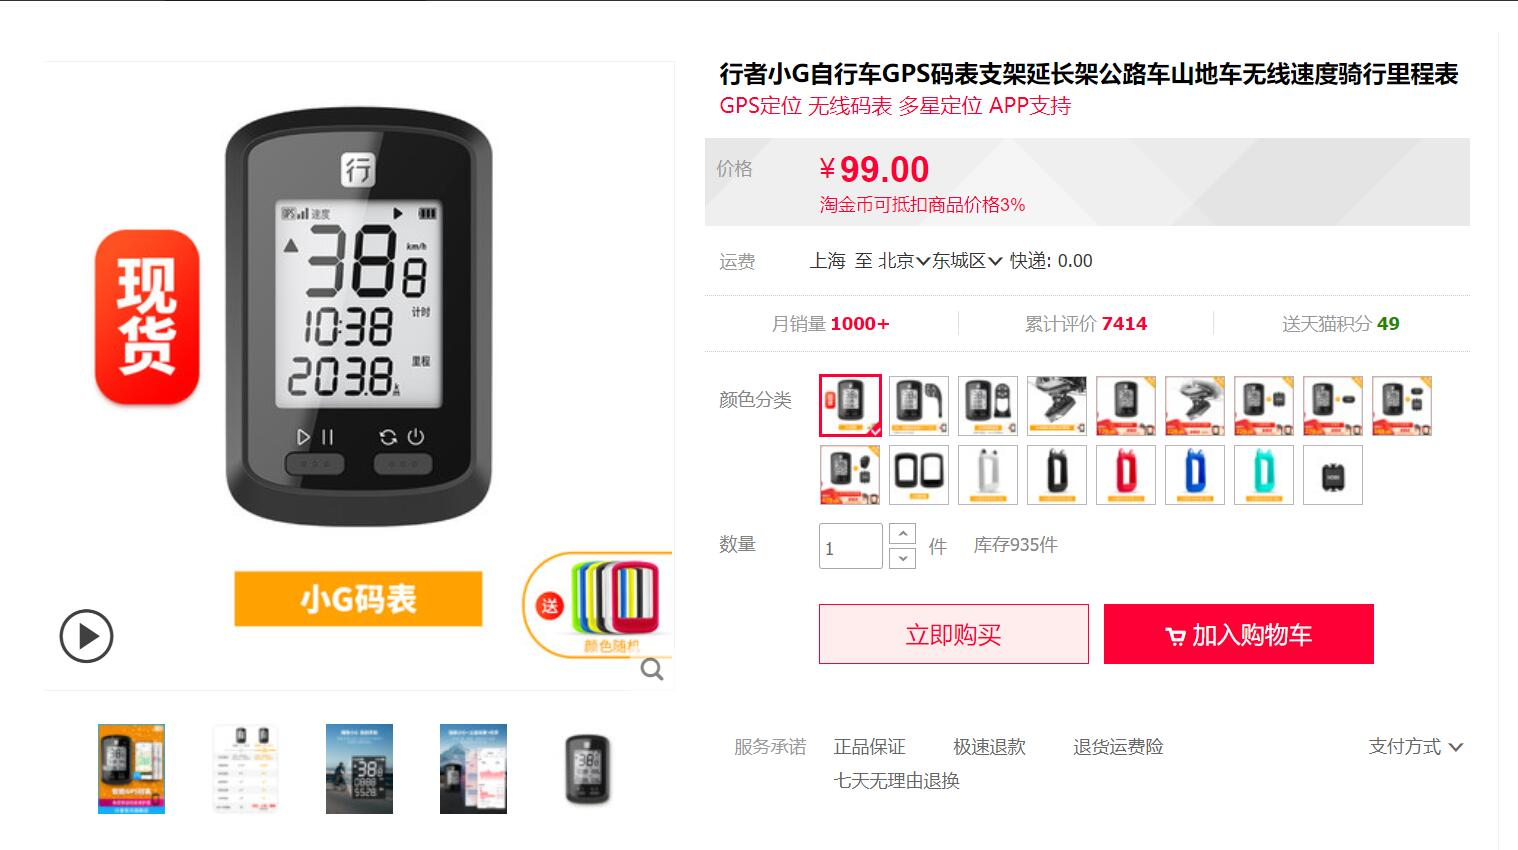
\includegraphics[width=0.7\linewidth]{fig/小G}
            \caption{}
        \end{figure}
        
        如果需要心率计和踏频计来辅助训练的话,可以购买行者的''小G+``并购买相应配件。

        
        如果想走向专业的话,还是要入佳明的。可以去了解了解一下佳明520,530,830。再贵就不推荐了。注意:如果选择要买专业码表,那么还应该有一个功率计和心率带来配合使用!因此考虑预算的时候还要把功率计和心率带的花销考虑进去。
        \item 功率计
        
        \item 心率带
        
        \item 踏频计
        
        \item 驮包 

        长途骑行不建议背包,对后背和肩膀的压力很大,建议把行李放在驮包中。
    
        驮包可大可小,理论上应面对不同的场合选择不同大小的驮包,但由于经费等问题,往往我们只会有一个大驮包。在需要拿的东西比较少的时候时,可以把书包放在货架上用绑绳绑好,即可免去购买小驮包。
    
        在爬一些很陡的坡的时候(参考太舟坞最后一个坡),如果货架上有一个大驮包,车辆很容易翘起后轮,造成摔车。这种时候应推车前进。
    
        推荐产品:
    
        淘宝店铺名称: GDW高大威装备
        \begin{figure}[H]
            \begin{center}
            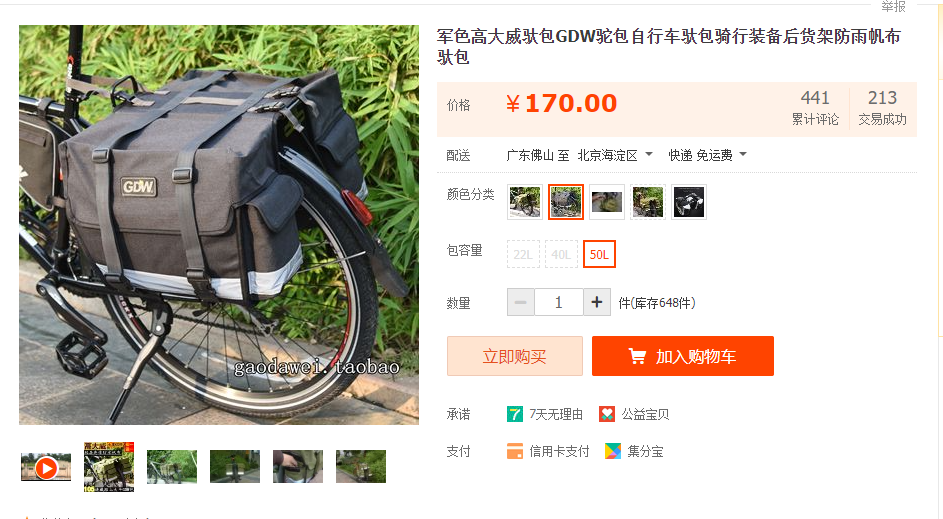
\includegraphics[scale=0.3]{fig/高大威_驮包.png}
            \end{center}
        \end{figure}
        淘宝店铺名称:波尔兄弟 单车户外运动装备
        
        犀牛驮包

        参考价格:¥100~200
        \item 手电筒 
    
        一般由队长负责携带,在需要夜骑的时候分发给大家(两人一个)。

        \item 尾灯
    
        一般由队长负责携带,在需要夜骑的时候分发给后骑。

        \item 车撑
        
        诚然,车撑在一定程度上有损车的美观度,但多人长途旅行旅行(暑期),有车撑会方便的多。不过一定要买质量好的车撑,货物多的时候车撑很容易坏。
        
        \item 货架

        货架的挑选有很多细节:有预留孔的,没有预留孔的,所有的预留孔都有的,有的孔有有的没有的,快拆的非快拆的,实心的非实心的,带坐垫的不带坐垫的,带挡板的不带挡板的。

        像下图这样的,就是没有挡板的货架。平时往上面放个东西还可以,但是不能放驮包。因为驮包的两侧会和轮胎发生摩擦。所以如果想走暑期的话,这样的货架可以不用考虑了。(除非你走暑期不带驮包?emmmmm,大胆的想法)
        \begin{figure}[H]
            \centering
            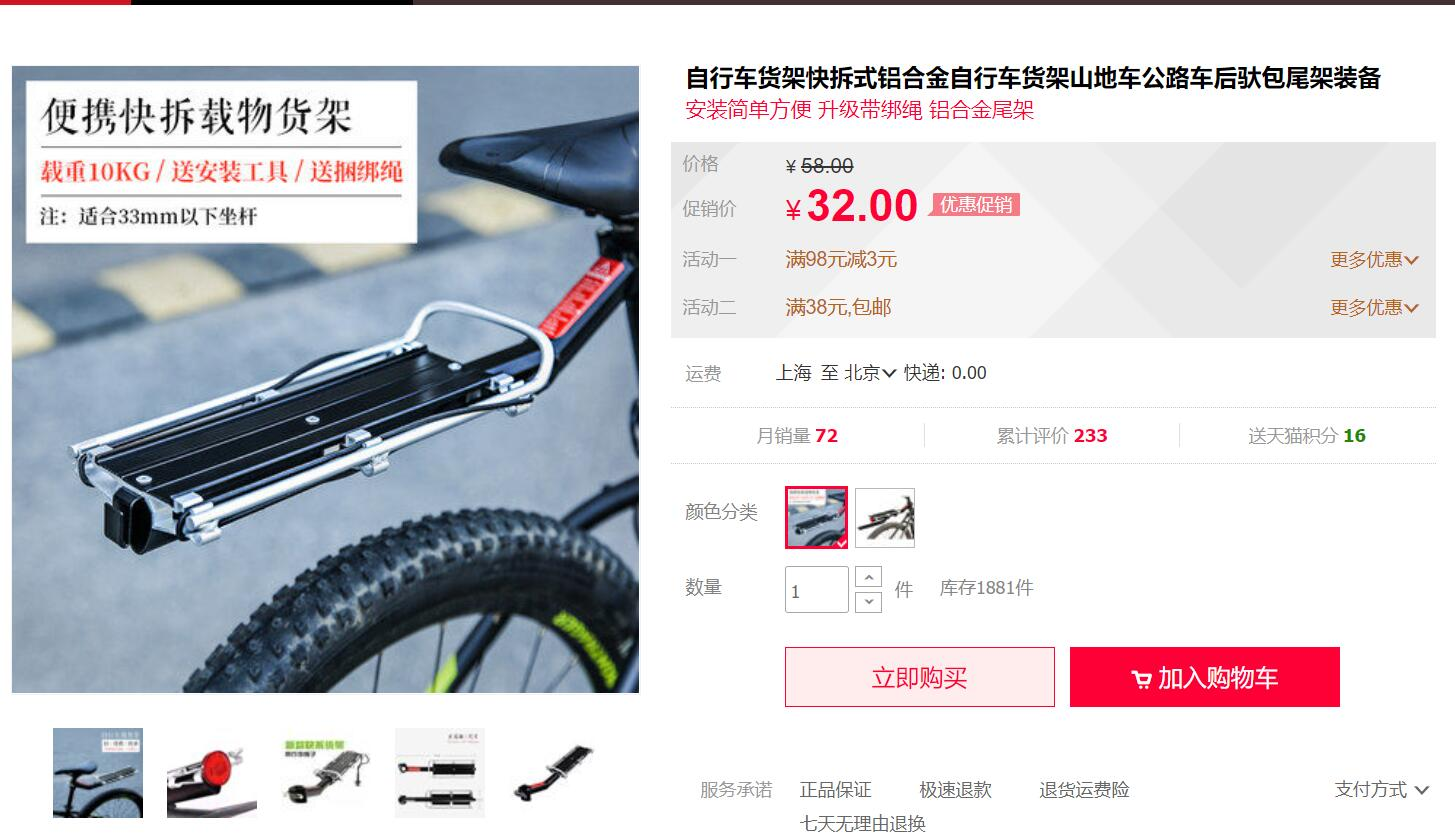
\includegraphics[width=0.7\linewidth]{fig/货架_无挡板}
            \caption{无挡板的货架}
        \end{figure}
        
        如果自己愿意的话,可以在网上一点一点挑,但是仍然存在买到之后不能成功安装甚至不能退货的可能。最省事的办法是去车店,但是肯定会贵一点。
        
        在淘宝下单前,应给店家车的照片并告诉车的型号,而且还要跟店家确定如果不能安装成功,能否退货,不支持退货的一定不要购买!!!

        参考价格:¥30——¥130

        不推荐的淘宝店家:
        
        GDW高大威装备——我自己在他们家买过一个货架,发现安不上,居然不给退货!!!不过我当时也懒得跟他多叭叭,好好沟通的话应该也会给退货的。
        
        \begin{figure}[ht]
            \begin{center}
            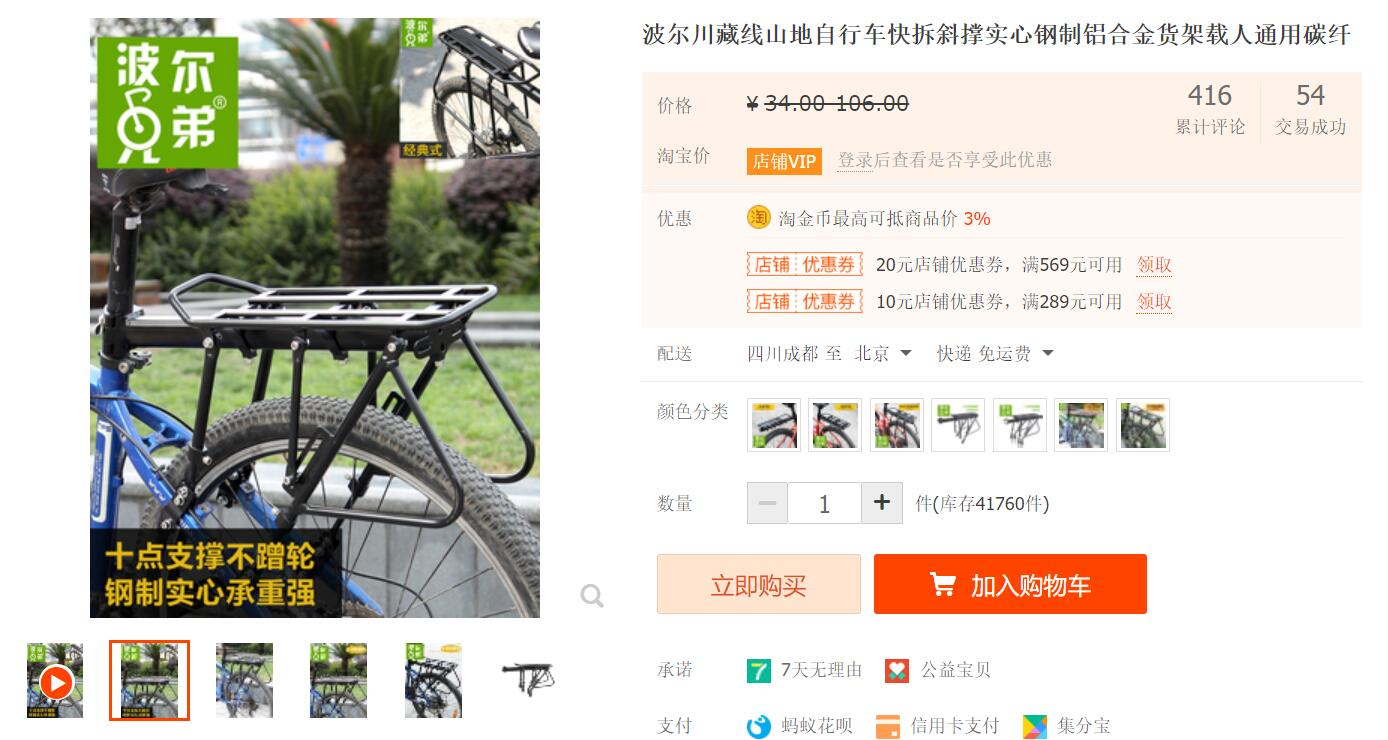
\includegraphics[width = 0.8\textwidth]{fig/波尔兄弟_货架.jpg}
            \end{center}
        \end{figure}

        \item 手机支架  
    
        价格大约在30r左右。

        根据个人习惯选择是否安装手机支架。前骑必须要有一个。

        即使你不需要手机来导航,手机支架也有它的好处。它可以把你的手机放在一个你比较方便看到的地方,也不需要额外的手来抓着它。如果放到口袋里,很容易漏接电话。而且放在手机支架上,放歌也比较方便。

        差的手机支架可能有以下问题:
        \begin{itemize}
            \item 手机支架安装不牢,乱晃
            \item 原本卡的很紧的手机随着旅途的颠簸会逐渐松动,甚至掉落
        \end{itemize}

        推荐的产品

        淘宝店铺名称:rockbros旗舰店

        \begin{figure}[H]
            \begin{center}
            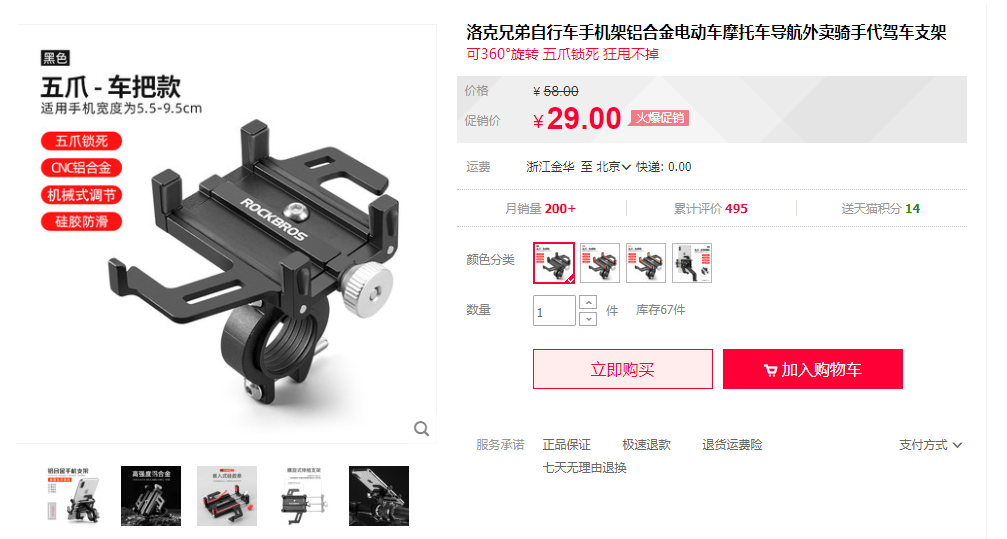
\includegraphics[width = 0.8\textwidth]{fig/洛克兄弟_手机支架.png}
            \end{center}
        \end{figure}
        不推荐买塑料的,感觉不是很靠谱。

        \item 坐垫
        
        如果刚开始骑长途车,往往会感觉屁股很疼,这时候可以考虑买一个坐垫。但事实上,如果选择了一个很软的坐垫,屁股或许没那么痛了,但这会在你每次踩踏的时候发生泄力,所以会让你更累。
        
        更好的处理方案是,练就一个铁屁股。
        \item 管包 
        
        根据个人习惯选择是否携带。
        \item 雨衣    
        
        如没有携带雨衣,可向车协购买一次性雨衣
        \item 护膝
        
        护膝分成两种,一种是运动护膝,一种是保暖护膝。运动护膝适用性比较广,在一定程度上可以减少膝盖的磨损。保暖护膝往往之后在寒冷的天气里才会使用。

        \item 水壶架
        
        一般的车会有两个安水壶架的地方,小一点的车只有一个。

        水壶架的大小也是一个需要注意的点,小水杯放进大水壶架里可能会掉(一般不会掉,但是在过减速带或者xc的时候掉的可能性大大增加)。大水杯(比如脉动)放不进大水壶。最省事的判断大小是否合适的方法是带着水壶去车店看看实物。


        
        还有的水壶架是可以绑在车身上的,不需要使用预留孔,换句话说可以让你装更多水壶。

%        \begin{figure}[htp]
%            \centering
%            \label{fig:}
%            \includegraphics[width=0.%7\linewidth]{fig/免打孔水壶架}
%            \caption{免打孔水壶架}
%        \end{figure}
        

        \item 水壶
        
        有专门的骑行水壶,大约是四五十元就可以买到。骑行水壶的特点是可以单手操作,省去了拧去瓶盖之类的操作。有的是需要挤压的,有的是吸的,有的是需要把盖子咬下来的。

      \begin{figure}[htp]
           \centering
           \label{fig:99}
           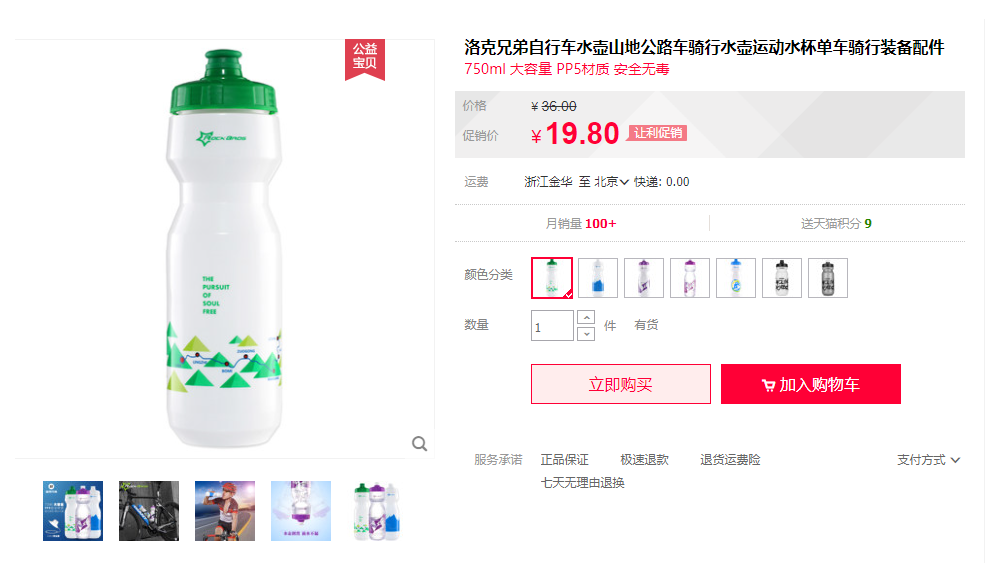
\includegraphics[width=0.7\linewidth]{fig/洛克兄弟-水壶}
           \caption{洛克兄弟水壶}
       \end{figure}
       
    \end{itemize}
\section{生活用品} 
    \begin{itemize}
        \item 充电宝
        \item 小零食
        \item 洗面奶
        \item 牙刷
        \item 防晒
        \item 洗衣粉
        \item 电吹风
    \end{itemize}
    \section{团队用品} 
    \begin{itemize}
        \item 后骑包
    
        一般由后骑携带。后骑包中应至少包括26,27.5寸的内胎各1个、撬胎棒3个、组合1个、磨胎棒2个、胶水1个、补胎贴6个

        \item 队医包    
    
        一般由队医携带

        \item 插排
        
        住宿的时候有时需要给大量设备充电:充电宝,手机,车灯,码表。而且双人间里可能会住进来三四个人,所以有一个插排还是很有必要的。
        
        推荐使用这样的方形插排,携带方便,并且有usb插头可以使用。

        \begin{figure}[H]
            \centering
            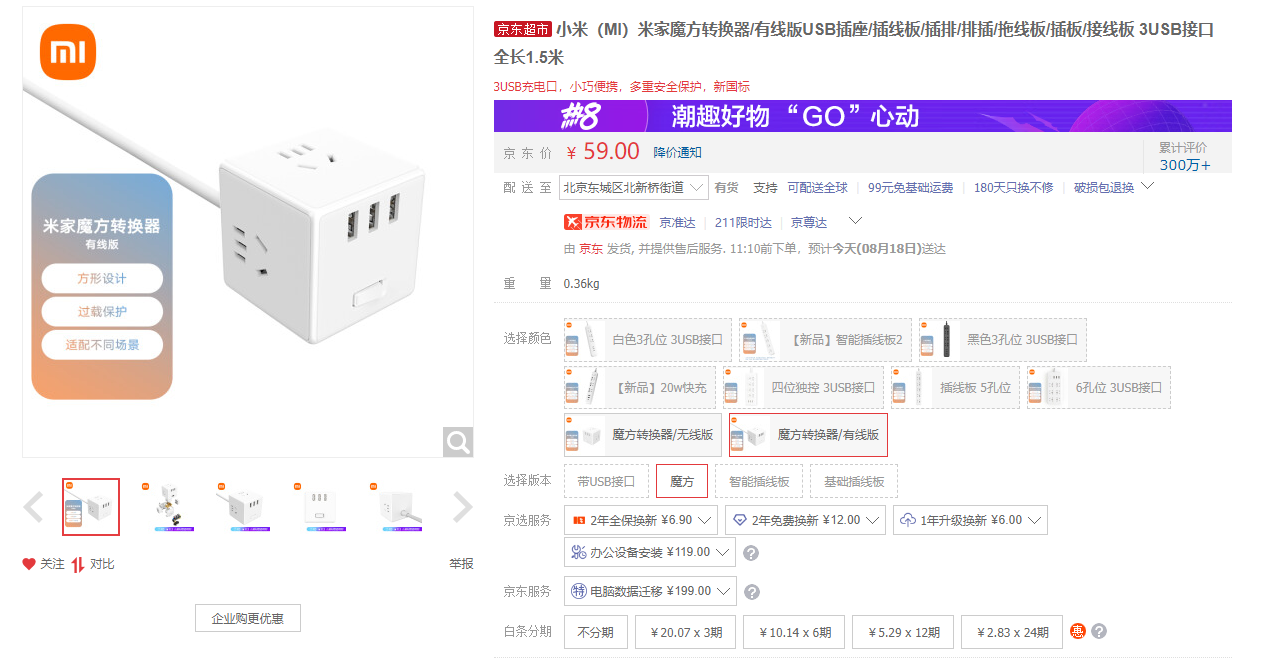
\includegraphics[width=0.7\linewidth]{fig/插排}
            \caption{小米插排}
            \label{fig:}
        \end{figure}
        

        \item 垃圾袋   
    
        一般由后骑携带

        \item 防潮垫 
    
        防潮垫的作用很大,它可以让我们在大多数时候都能坦然的坐在地上而不用担心着凉或者弄脏衣服。另外,它也可以让我们睡上一觉。

        推荐尺寸:大小:120cm*200cm 厚度 6mm

        参考产品:
        \begin{figure}[H]
            \centering
            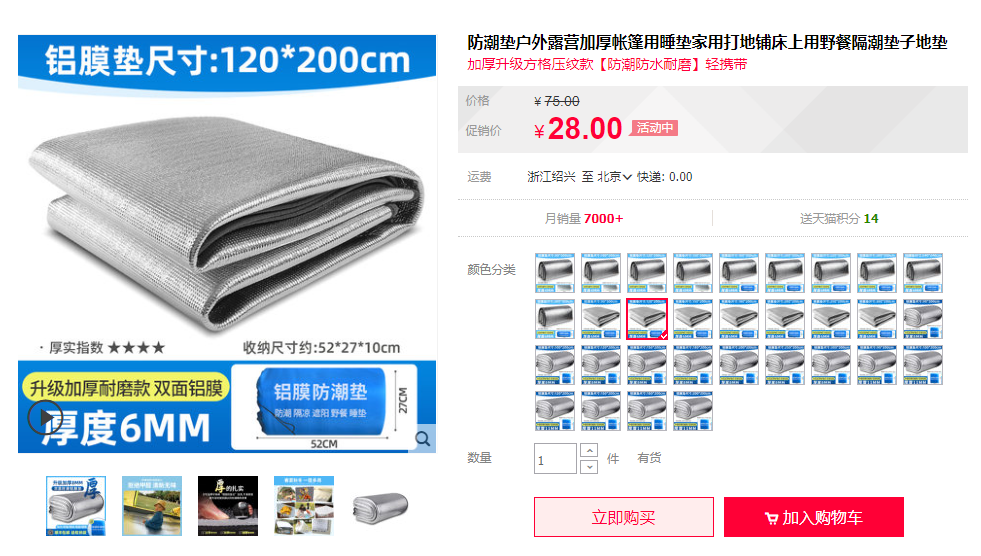
\includegraphics[width=0.7\linewidth]{fig/防潮垫}
            \caption{防潮垫}
            \label{fig:}
        \end{figure}
        

        \item 补胎工具
        \begin{itemize}
            \item 磨胎棒
            \item 撬胎棒
            \item 补胎片
            \item 补胎胶
            \item 打气筒
        \end{itemize}
        \item 棋牌    
    
        一般由后骑携带
        \item 记号笔
        
        方便在一些不便于用水性笔书写的地方做好标记,比如:
        \begin{itemize}
            \item 在防潮垫上标注正反
            \item 在相同的骑行水杯/驼包上标注其主人
            \item 在墙上写字留念\footnote{注意:应当在专门的留言墙或在墙壁主人允许的墙体下写字/绘画}
        \end{itemize}

        \item 哨子
        
        \item 扎带

        装车的时候会用到,车上的线也可以用这个来绑。

        \item 旗杆:两米一到两米二
        
        旗杆可以在出发地进行购买,可以选用的材质为:不锈钢,PVC管,竹竿。其中不锈钢管的重量较大,不做推荐。
        
        \item 大旗(队旗/会旗) 推荐尺寸:建议比144cm*96cm 小一号。(还没有搞清楚应该用多少的)
        
        注意:如果旗杆短且旗帜比较大,在爬坡的时候容易出现旗子卷进后轮的情况。
    \end{itemize}

    \section{自行车} 
    
    没有自行车也没有关系,可以跟实践部租车,一天10元。不过我们还是建议拥有一辆自己的自行车。目前车协中最多人骑的车是美利达的挑战者300,价格大约在3000元左右。

    如果经验不是很丰富的话,不建议在网络购买。

    每年的春季学期和秋季学期我们都会组织一波团购,到那时一起买车的话会便宜很多。

    参考车辆:

    捷安特xtc800,美利达公爵600,美利达挑战者300
\section{救命装备}
\begin{itemize}
    \item 保温毯
\begin{figure}[H]
    \centering
    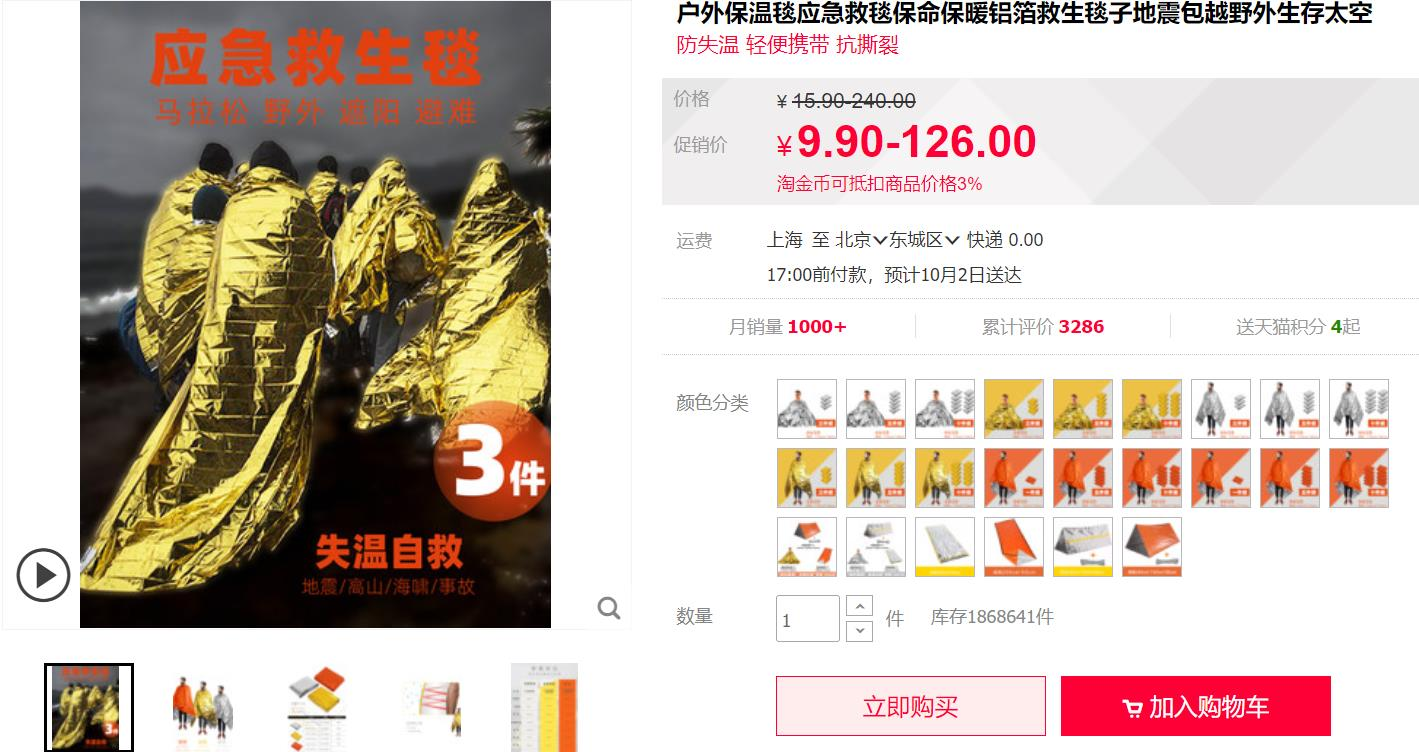
\includegraphics[width=0.7\linewidth]{fig/保温毯.jpg}
    \caption{保温毯}
\end{figure}

体积小巧,一般用于低温环境下,可保持自身大部分热量不散发,维持体温。此外,它在光照下具有强烈的反光,更容易让营救的人员发现。

保温毯正确使用方法:\href{https://www.bilibili.com/video/BV1yf4y1h7Hh}{bv1yf4y1h7Hh}
\item 对讲机

可以在不需要任何网络支持的情况下,进行谈话。适用于网络不稳定,经常穿梭无人区的暑期队伍。购买民用对讲机即可。使用体验非常好,方便,打开后摁住就可以说话。

\item 氧气瓶

高原旅行使用氧气瓶可快速缓解高反。氧气瓶不能带上火车飞机,只能当地购买。氧气瓶规格按需购买。
\end{itemize}
\chapter{交通工具违禁品}
\section{飞机}
\subsection{禁止随身携带或托运}
\begin{itemize}
    \item 枪支、军用或警用械具(含主要零部件)及其仿制品
    \item 爆炸物品,如弹药、烟火制品、爆破器材等及其仿制品
    \item 管制刀具
    \item 易燃、易爆物品
    \item 腐蚀性物品
    \item 毒害品
    \item 放射性物品
    \item 其他危害飞行安全的物品
\end{itemize}
但是嘛,这些东西你一般不会带,也没有。
\subsection{咱们需要注意的}
\begin{itemize}
    \item 茶水饮品:茶水饮料是不能携带上飞机的,进安检时必须将杯子液体全部倒出来。
    \item 水果刀:一般刀刃不超过6cm的水果刀,只能通过行李托运,不可随身携带。
    \item 手机电池:手机电池只能装在手机中随身携带而不能通过行李托运,移动电源不超出20000毫安可以随身携带。
    \item 化妆品:对容量大于100ml的化妆品建议将化妆品放于行李托运。防晒喷雾、洗发水、沐浴露等小于100ml可随身携带。
    \item 药品:固态药品、少于100ml的液态药品可以携带。单件超过100ML的液态药品,而且必须在飞机上服用,需要医院证明、处方等。
    \item 酒类:酒类不能随身携带,可托运。酒精度24度以下(含24度)的酒类物品,托运的数量不受限制。酒精度在24度(不含24度)至70度(含70度),托运的总量不得超过5升;酒精度在70度(不含70度)以上不能托运。
    \item 五金工具:不能随身携带,可托运。
    \item 液体喷雾发胶,可以托运.发蜡一般是分两种的,膏状发蜡,可以带上飞机;泡末发蜡,像摩丝一样进行压缩罐装的,是易爆品,禁止携带和托运。(不会有人带着发胶走暑期吧)
    \item 不能带氧气瓶。 
\end{itemize}
对于旅客提出需要暂存的物品,民用运输机场管理机构应当为其提供暂存服务。暂存物品的存放期限不超过30天。民用运输机场管理机构应当提供条件,保管或处理旅客在民航安检工作中暂存、自弃、遗留的物品。
\section{高铁/火车}
\subsection{禁止携带}
与飞机大致相同,不一一列举。
\subsection{咱们需要注意的}
\begin{itemize}
    \item 禁止携带刀尖角度小于60度,刀身长度超过150毫米的各类道具。其他刀尖角度大于60度,刀身长度超过220毫米的各类刀具。
    \item 限带两盒安全火柴、两个普通打火机。
    \item 自喷压力容器不得超过120ml,(我们的防晒喷雾就是这个)。
    \item 氧气瓶也不能带。
\end{itemize}
\section{长途汽车}
\subsection{禁止携带}
与飞机、高铁、火车大致相同,一般违禁品咱都没有。
\subsection{咱们需要注意的}
\begin{itemize}
    \item 限带包装完好的白酒2公斤。
    \item 限带打火机2个。
    \item (氧气瓶)
\end{itemize}
对于长途汽车违禁品的信息不多,但是易燃易爆的咱就别带了,夏天温度高,在行李舱里容易发生危险。
\chapter{各部门实用信息}
\section{宣传部}
\begin{itemize}

\item 百度百科:\href{https://baike.baidu.com/item/%E4%B8%AD%E5%9B%BD%E5%86%9C%E4%B8%9A%E5%A4%A7%E5%AD%A6%E9%98%B3%E5%85%89%E8%87%AA%E8%A1%8C%E8%BD%A6%E5%8D%8F%E4%BC%9A/1861065?fr=aladdin}{中国农业大学阳光自行车协会}
\item 搜狗百科:\href{https://baike.sogou.com/v45363368.htm?fromTitle=%E4%B8%AD%E5%9B%BD%E5%86%9C%E4%B8%9A%E5%A4%A7%E5%AD%A6%E9%98%B3%E5%85%89%E8%87%AA%E8%A1%8C%E8%BD%A6%E5%8D%8F%E4%BC%9A}{中国农业大学阳光自行车协会}
\item 哔哩哔哩:\href{https://space.bilibili.com/266648273?from=search&seid=13669577487834144080}{阳光车协}
\item 新浪微博:\href{https://weibo.com/u/2026266875?is_all=1}{阳光车协}
\item 邮箱1:sunnybikefromcau@163.com
\item 邮箱2:ygcxbgs@163.com
\item 行者骑行:中国农业大学阳光车协
\item 抖音短视频:CAUsunnybike
\item 微信公众号:阳光车协
\item 微信主页君:ygcx20010315
\item QQ主页妞:1757504646
\end{itemize}
\section{活动部}
推荐使用行者骑行制作路书,网页版:http://www.imxingzhe.com/

晚训相关内容请看第 \pageref{sec:晚训} 页 
\section{实践部}
\begin{table}[htbp]
    \centering
    \begin{tabular}{|l|l|}
    \hline
        车店/车棚 & 联系方式     \\ \hline
        东区美利达 & merida\_xyl      \\ \hline
        西区美利达 &     \\ \hline
        北辰捷安特 & meng-yang555555    \\ \hline
        车棚 & 13520061361     \\ \hline
    \end{tabular}
\end{table}
\begin{table}[H]
    \centering
    \begin{tabular}{|c|c|c|c|c|c|}
    \hline
                                   & 零售价        & 车型           & 零售价        & 车型           & 零售价       \\ \cline{2-6} 
                                   & 1398       & 探索者100       & 2098       & 达卡616        & 898       \\ \cline{2-6} 
                                   & 1798       & 探索者300       & 2698       & 达卡620        & 1098      \\ \cline{2-6} 
                                   & 2198       & 探索者500       & 3398       & 达卡620D       & 1198      \\ \cline{2-6} 
    \multirow{-5}{*}{车型}           & 2698       & 探索者X         & 3498       & 达卡624        & 1298      \\ \hline
                                   & 3398       & 探索者600       & 3998       & 达卡624D       & 1398      \\ \cline{2-6} 
                                   & 3998       & 克罗威90        & 1798       & 知音           & 1398      \\ \cline{2-6} 
                                   & 4998       & 克罗威100       & 2598       & 达卡624HD      & 1598      \\ \cline{2-6} 
    \multirow{-4}{*}{挑战者300}       & 7098       & 拓荒者2S        & 2698       & 安琪N3         & 1298      \\ \hline
    挑战者SL1                         & 4098       & 拓荒者1S        & 2198       & 飞翔20         & 1298      \\ \hline
    挑战者SL7                         & 7098       & 野狼1          & 2298       & 飞翔30         & 1598      \\ \hline
    维多利亚500                        & 1698       & 野狼2          & 2598       & 飞翔50         & 1998      \\ \hline
    维多利亚700                        & 2698       & 野狼5          & 3698       &              &           \\ \hline
    维多利亚800                        & 3398       & 野狼7          & 4698       &              &           \\ \hline
    维多利亚600                        & 2098       & 朝圣           & 2798       &              &           \\ \hline
    莱得91                           & 1498       & 天籁N3         & 1598       &              &           \\ \hline
    斯特拉92                          & 1998       & 铁马           & 798        &              &           \\ \hline
    斯特拉93                          & 2998       & 郁金香          & 798        &              &           \\ \hline
    95D                            & 4298       & 安琪           & 798        &              &           \\ \hline
    斯特拉95                          & 3998       & 美琪           & 798        &              &           \\ \hline
    斯特拉碟刹大王                        & 6098       &              &            &              &           \\ \hline
    \end{tabular}
    \caption{21年度美利达主要部分车种零售价表7月12日(西区美利达)}
\end{table} 
\section{办公室}
\subsection{购买保险}
可在下面两个网站购买保险:
\begin{itemize}
    \item 美骑保险 https://bx.biketo.com/
    \item 百川保险 https://www.besttrav.com/doc/bc-introduction-fwnew.htm
\end{itemize}

\chapter{车协管理经验}
\section{执委会}
\subsection{秋季学期第一次执委会 2021.9.5}
开学后马上就要召开第一次执委会,会议应当包括以下内容:
\begin{itemize}
    \item 找秦皇岛负责人。
    \item 开展招新活动,刷楼,海报,百团大战,收新老会员会费,新生见面会,招新推送,恢复晚训的推送。
    \item 秦皇岛前的骑行活动。
    \item 换届:换届的推送,物资的交接,在车协历年路线图中添加今年的路线。
\end{itemize}



\subsection{秋季学期第二次执委会 2021.10.9}
1.2021年招新总结及收尾 A.新生见面会——人数共招新141+人 B.招新并未停止——冬训、暑期拉练仍旧会有新生加入; C. 海报+招新视频;三版海报;多部视频,公主楼大屏幕播放 总结: 很辛苦,很优秀 附:2021年招新开销: \notes{把这里改成跟第一次执委会的样式}

1)执委提出招新意见关注社长群消息,按要求领物资;

2)新生见面会人数少,零食剩余,原因与其他组织活动冲突,不决定改变时间;

3)凤凰岭活动百团之前,地点可换,加油探路;

4)刷楼海报数量注意,省着发,多印点;

5)刷楼尽早。西区、烟院能省就省;

6)军训期间——提前准备!形式+礼物(西瓜、批发小零食、赞助等);

7)烟院招新:躺尸式摆摊招新,只做一天

希望未来:百团易拉宝,推送型,讲解详细的,比海报更具象。烟院招新易拉宝 

2.秦皇岛 总结:干货性总结,重点前期准备,10月30号23:59截止。重点在人数,新老比,男女比例。慎重分仨队,多关注体力,太离谱劝退。执委间配合沟通需加强。队长准备好处理突发情况。李籽林事件,发烧状况。摔车较重可直送夏阿姨家。 详见队长总结。

3.各部门总结这一个月的工作 + 规划 

1)办公室 东区: 招新拉新人,收会费,统计工作。两次活动,报名表、策划。百团物资、其他物资。

活动名单日常办公室负责,秦皇岛队长负责。策划队长负责。活动职务安排队长负责。 

西区:没做什么。队医包,没做什么。

队长前期工作,分工明确,前期工作间配合。 

会长: 秦皇岛报名表需更精致,报名表审核随机@2~3人,至少回复个好! 

2)实践部 郭正伊:限制人数,直接以车给限制。 

会长:补充新胎(美嘴、法嘴别省事)多整点,补好的胎接着用,第二次扎就可以放弃,后骑包,

马睿恒:车辆大排查,统计,新牌。清理车辆,车棚练习。团购11月5日。 

3)宣传部 陈嘉瑜:八九篇推送、俩食品。审查问题,先跟个人说。 

严天龙:工作提早说。说明白。 

4)活动部 肖心宇:啥也没干。确实水!  

游安旭:没干活! 

会长:活动部核心。

之后活动自觉点。会长助理。之后统领。

要对活动有期待。团委挂名不重要!我是核心、灵魂。活动部确实没干啥!

72周年可夸。期待新活动,带新活动! 

5)外联部 杨艳周:拒绝奶茶店,谈了个餐饮(蛋糕店),自己找上门来到不靠谱。

拉赞助说完了。跟峰云社取经,没学着啥。

外联积累。现在没啥大动作。

洛克兄弟继续谈,要大家商量。

银杏林外联部、活动部合作,有更好活动,可替换掉。

其他高校车协联动,没啥实质性的,联动太麻烦就没啥意义了。 

校内社团外联,重点红十字会,两家多合作,队医培训找他们。

加强队医培训。药品可以跟他们聊聊。 

肖心宇:从红十字会招新,多跟外校mm联动。格局打开,着眼北京,异想天开。 

会长:重点红十字会,外校联动不用太关心。

赞助多考虑,先发执委。 

4.接下来的活动 时间线:10月15日夜游京城  队长:王上林、陈嘉瑜,策划以前的    不带旗         10月16日八大处  队长:肖心宇             (10月10日12:00出策划给宣传部,周一中午出推送审核,下午2:00出推送) 10月23日银杏林 队长:严天龙  外联加油!   提前一周找队长!!!!! 10月24日暑期报告会暨冬训宣讲会 冬训队长马睿恒  海南!!!     主要负责人游安旭 借教室、零食,所有暑期队长PPT,冬训队长PPT,先报告后宣讲,冬训选拔方法PPT理事会负责。     去督促宣传部做简短的报告册,找老人督促要材料,十来页A4纸,不用太正式,征集时间截止13日,定稿时间17日。 10月30日香山防火道  11月07日 冬训拉练开幕  车牌宣传部设计,实践部负责 收集照片制作明信片外联负责 宣传部把金主的尾巴做精致 外联多跟金主聊,转发推送,宣讲恰饭……多和爸爸聊,哄好了钱都好说,要可持续发展 多找新人聊天!!!!!!!!!  5.冬训 提上日程,活动部安排''积分``''预告``''队友互评``''晚训``等等,在晚训期间了解大家的性格,让阳光们了解''冬训``这个活动。 
\subsection{秋季学期第三次执委会 2021.11.07}

1. 总结秦皇岛后面的活动:

夜游京城,八大处,冬训宣讲会,洗车 八大处:严天龙;八大处可能短,面积小;明年八大处还可以考虑其他的活动 洗车:太乱,游安旭:即使分组,还是很乱,工具找不到;执委来的很乱, 建议:分时段安排执委(很重要),不拆链条,简化秦皇岛的洗车,时间观念,流水线,检车的时候着重强调车上物品,实践部联系借车的时候问一下车主车上贵重物品(人多就不要拆链条,一般秦皇岛活动之后,没必要带新人教很细,之前的洗车是没有拆链条,以后义乌修车活动再教)  夜游京城:回来的时间有点晚,明年不要刷奥园,不走那段路,有时间去前门(明年要去);路线问题,今年的路线挺好,但是明年再说改进路线,前骑应该问''人齐了吗``(最重要的)''再问准备好了吗``。  冬训宣讲会:明年可以提前到六点半,明年争取公三招聘大厅  太舟坞:挺合适的活动 

银杏林:明年如果有这个活动,可以找一个替代的 

2. 秦皇岛之后除了洗车的周末,其他的每个周末都要安排骑游活动,夜游京城那周末的是两个活动。 3. 拉练:由于封校,2021年冬训拉练无法正常进行,采用其他活动替代。

把跑步、活动形式细化-具体到队长、项目 跑步放在东区,定向放在西区,顺序:定向,跑步,定向,跑步 定向:一队7人左右,分三队,一张地图,收手机,四个点,不同的地点出发,要报名表,策划,三个队伍都有零食奖励,第一名的队伍先选零食以及积分1分,第二名0.5。 跑步:不定向的周,只跑步,2+13或者2+15(波比跳不方便) 体测:目前的考虑是男生6公里6分半,女生稍微少一点慢一点,配速7分左右 4. 更换车牌:实践部找商家,问要求,这样宣传部才能设计,下学期出活动的时候戴上。
 
\subsection{秋季学期第四次执委会 2022.1.1}
1.	回顾冬训前期准备

① 蟒山拉练,可以安排午饭,燕山文化广场附近村,放坡下来吃饭再回去;爬坡练得少,体力可能行,骑行技巧缺少;队员熟悉度低。(往年一次不过无补测,今年疫情问题少拉练可补,具体情况看队长与实际情况)。

② 安全意识,新队员的安全意识还不够:绑带、放坡书包掉停靠了左边。   

后续需要对队员的安全意识进行强调提醒,2022找回状态~

③ 宣传部收集冬训体测照片视频★

④ 冬训队队内没有私约晚训,本应该有(天气冷,但是不能荒废),想到就干,权衡一下,克服一下。

⑤ 机票,住宿,路上多拍点高质量好些的照片视频(成队人数:14)

⑥ 冬训拉练执委也要多关心多参与

⑦ 冬训体测花销200左右,租车新成员免费,只需要出油费

2.	冬至包饺子

① 提前一周准备

② 灿灿学堂,只需要工本费,无场地费,人均26元

3.	车棚(开学两周内处理完,实践部)——车牌(实践部\&宣传部,开学整好)——租车钱

① 统计车数,统计数与实际停放数比例不要差太大,老会员(可能常借车,自己不常骑的)的适量可多放(提前和阿姨打好招呼)。什么车停半年、停一年,尽量清楚,表格

新老大群里公告说一下情况,统计拉车主群

② 新长久停的要提前统计,补钱。废旧车处理

③ 120元再谈谈,尽量符合阿姨心理预期——统计车数

④ 先把这学期的价钱结了,新且停车棚的补钱

⑤ 寒假把车牌设计出来1.15.23:59(严天龙),下单(商家找好了,找王上上,若其他问题严天龙可以重新找,下单),排号(直接找新车主入群),挂牌(开学,检车发一部分,余下直接帮他们挂上去)

⑥ 学期底统计,所有表发给办公室,办公室统计名单和钱,发给实践部,实践部把钱发给车主,1月15前号完成

4.	洛克兄弟的大旗★

洛克兄弟那边提供设计,我们整旗;1.25前得设计图,靳维轩问

5.	工具箱★

下学期开学实践部整理,标签

6.	周边、文化,B站视频上传★

① 周边推送,甲鱼,下学期有活动再发

② 文化推送,惊鸿,寒假完成,下学期发布

③ 暑期视频,队伍视频先下架,再与车协合作上传

7.	十佳社团·问题反思

① 材料?

② 不改变自我前提下,有这个意识,不用太刻意,把握方向,靠拢一下党向、公益性(答辩时注意注意注意)

③ 实践、路线

④ 以后暑期注意一下,为社团长期发展考虑

⑤ 活动中都带上团旗,一起拍照(黄洪洋)

⑥ 和学校团委互动太少,团委方面组织的视频可以参与一下,金色希望、五月花海、校庆嘉年华的回顾推送发到团委那边,要重视学校的活动,别水。

8.	跑步、拉练执委别摆烂,更积极参与点,尽到自己的义务,''不能光寻思着玩``,下学期热情点

9.	暑期

(1)	个人意愿/想法/川藏线

油:巴拉巴拉···搭档—预期严天龙,路线—川藏318

龙:搭档—油

马:若凑齐三条队,就走川藏,

周:简单的线,实践或短途,带女副队

郭:实践,不确定

林:不确定

一个队伍不能只有一个女生;

川藏线,商业化有,但是自然条件确实恶劣,多想点

寒假找心态,想清楚,路线、食宿、预算、队伍、阵容、准备

\subsection{春季学期第一次执委会 2022.3.6}

第一次执委会会议记录

暑期

1、游安旭-骑行队:非常渴望走这条线,个人选择,虽然商业化很明显,11个或者12个HC坡,川藏线;从成都出发骑到拉萨,25天版,再加上从北京到成都有28到30天,预留出一定的时间;攻略有很多;队费不算景区,预计最少4000(不够);预报名还是会有,但是今年要避免分散队伍,预报名开始到预报名结束之前所有队长不知道每个队都有谁;体测标准按照去年的标准,所以不用怎么改,跑步体测的标准不能降;队伍建设,成队之后对内约跑步,约活动,尽可能聚在一起。没成队之前,在大群多私约,梳理整体队长的形象。(关于探路问题。。。换届问题。)

2、小马,wss-实践队:路线选择:最美公路S201,G108,加上考虑周边的可以玩的景点,终点是九寨沟;包头是交通枢纽,北京直达,整条景观有变化;路书已经做完,有吃有住,每天100左右,不是很紧;爬升两万出头,主要是在后期的秦岭和九寨沟,前期不是很难,先易后难;从出发到九寨沟路程22天,九寨沟附近可以可以去别的地方玩,实践时间还不确定,暂定在四川做,在陕西部分做,今年的情况不是很清楚,正在问红十字会(可以用志愿抵消时长)还有学校,但是不是很急;有大城市可以追车。10-12人左右,最多14人(意见:倒着骑,但是九寨沟放在后面可能比较好,比较期待;尽量避开城市中心的路;沿途气候变化比较大,注意提前的准备,干湿差别比较大;实践做学校的比较省事;红十字基金会在全国各地有一些扶贫的基地,之前是联系他们在当地做实践;一定要问清)

3、杨艳周-短途团:从锡林郭勒-漠河,总长1500km,成队之后再商量要不要加上公路,最少连骑到休息总共20天,实际爬升会比路书很多,可以砍头可以去尾,时间控制在总共25天;越过大兴安岭之后会有景观的变化;时间可以参考塞北寻星的安排;漠河可以包车回去;尽可能避开疫情区;找副队长,双线培养清明前找人,发展新人;五一之前尽可能解决这个问题(提问:可能会有找不到住的地方,解决办法,从高德上找电话询问住的地方;可以坐车去北极村)

4、会长讲话:① 副队长问题——名义上的副队长成队之后选新人(给新人的这个称号),成队之前至少两个执委搭班组织一个队伍,为了培养新人的责任心,否则会新人参与不到前期的准备中,而且新人在一个队伍中占比比较多,可以提出更多的意见;杨艳周没有执委搭档,要么冬训队员,要么老人,要么执委,要么大四这群人,一定要选一个可以搭伴。(情侣上路会影响队长的决策,影响队长的理性思考,没得商量)② 里程问题:必须在暑期宣讲会上缩短几百公里,展示在PPT上1500公里左右,成队上路之后再商量,再加路线,考虑到新人的体力问题,最开始对自己能力不自信,所以不要把特别详细路书放上去。要与骑行队分开

清明:

1、由于农大不调休,今年可以时间长一点。

2、郭正伊、贺靖婷队长,一人找一个新人,带新人队长

3、清明之前如果解封的话,可以出去玩,景点选择:戒台寺,太舟坞比较合适,(最早3月20号解封)

4、清明活动(节的前两天都可以),十渡不怎么样,黄花城(可以办篝火晚会,所以向北大取经),还是两天的活动,不要办三天的活动,可以发前站准备篝火晚会 。

生日会,冬训报告会

1、流程:放视频,发抽奖券,活动开始,会长发言,冬训队长上台报告带队员,抽奖;后半段是生日会,放祝福视频,小游戏,然后理事会发言,揭幕路线,三个队长自我介绍,不用详细介绍暑期路线,唱会歌,吃蛋糕,合照(尽可能花里胡哨一样)。(3月20日晚上)

2、负责人:姚琳文,袁菁宏,主持人找一男一女,活动分的细一点,分给每个人,制定活动策划(3月11日),定教室,考虑公三招聘大厅(交给杨艳周,不行就借教室),可以申请外校人员入校,但是外校还没开学

3、锦上添花细节:可以放往年的会服,挂在墙上,找到车协20周年之前的会服,20周年会服,新一版的会服,大脸的会服(wss还有小马有),带个衣架。

4、宣传部:要单纯祝福视频,面向所有的新老阳光征集视频(发到邮箱),通过预告生日会的推送征集(尽可能省事,下周四晚上发出去),里面截止日期是3月16日(下下周三);办公室(3月7号晚上之前发邮件)要给所有的有联系的车协发公开邮件要祝福视频,都发车协的邮箱(3月16日是别的车协的截止日期)(发邮件注释横竖屏的格式,宣传部的需要格式,原话画质;发的邮件从原来发的邮件改);外联,细聊三个车协,北林,华科,蚂蚁,徐泽敏(烟院以及所有附近);海报,不用易拉宝,背景就是总路线,然后把三条线路加粗;关于邀请外校的,杨先跟他们联系;冬训报告会PPT(3月16日);生日报告会的PPT也要安排人做(主持人做)。

暑期宣讲会

1、去年是清明的最后一天,今年是清明的第四天(4月5号),礼拜二,这样大家都回来了,时间很充足,从简,没有花里胡哨的东西(零食吃剩的就行),答辩,实践部买车,不用游戏和抽奖——王上林负责,写策划,有那些事,谁负责,什么时候截止。

2、流程:暑期视频(B站都有视频),主持人宣布开始,直入主题,讲PPT,然后问问题,问完之后理事会介绍选拔方案,实践部买车团购(可以提前发团购推送(3月9号毛子交稿子)通知性质的,放个群二维码),推荐买车,最后答疑

3、装备可能之后会团购

春季招新

1、摆摊:规模比较小,可以老人带新人,可以拿暑期宣讲会的海报,先不订负责人,学校的
暑期的选拔

1、理事会总负责,理事会建预备群,不能建小群,冬训成队队员可以加1分

2、晚训积分:第一周是执委会负责,剩下四周找四个新人一人带三次,刚好一个新人加一分;队长一定要积极主动,给新人树立好的队长形象,让新人重视起来。

3、对外一致宣称没有补测,统一口径,第一次体测之后才说

4、拉练:第一次妙峰山;第二次,去年是潭王路(不限制),但是提前探路;第三次,五一原则上不能换,如果要换,必须同类型,单程130KM以上,爬升1500以上,有乐趣(要考虑新人的想法);第四次,去年是禅妙阳(可以换),参照原来的路线,拉练能安排午饭就安排午饭,但是尽可能;第五次,韭园,要探路

5、体测:五月底

6、积分:找新人记,同时培养下一个办公室主任。

7、有奖牌:写一个''妙``;还有奖品不管新老都要发

外联

1、大家的态度比较消极,对于赞助的态度应该比较正面的一种态度,要上心;例子,之前的报告会把赞助忘了,不能忘,现在着手 准备给洛克兄弟的履约报告,把活动的照片都放在上面,有意识收集照片,外联部要商量,每一项都要展示出来,每一个推送的链接都要放在上面,告诉他们我们做的还不错,态度一定要好。

2、所有的会的策划负责人,做PPT的时候,选主持人的时候都要着重提醒重视这个赞助,

3、冬训视频可以片头片尾加上黑底的logo,找这种大牌子的赞助是一件非常光荣的事情,一定要重视。

4、也可以多聊点赞助,在会旗上可以加logo

5、做会服的那家店给全国很多学校提供赞助,所以可以找他们聊,从下一届会服开始都可以加洛克还有这家店的logo

6、改正观念,我们影响力:推送,会服,会旗;通过影响力去赢得赞助是一件很光荣的事。

7、把新的工作交给外联部,方便外联部的传承,也可以联系打印店,参考一下往届花了多少钱。

8、外联问问洛克兄弟是否可以定做骑行服

换届

1、多找点接班人,看好人,多聊聊,多交流

2、多上点心,六月下旬换届。

培训

1、五一之前的一个下午(参加五一的一定要去):职务培训,队长培训,安全培训,越野和知识科普培训,活动部负责,

2、修车培训:和义务修车一起搞,以操代练,必须解封之后才能,四月中下旬才能搞

3、五月的花海,还要和冬奥有联系,修。。五环车,实践部负责,
文创活动

1、可以挂坠(艺术字)

2、''拐个弯就到了``(三角的路标);圆的红色路标(''当心放坡``);''山地车如何拉爆公路车``

3、可以网上找梗图,自动填字

4、赵瀚坤负责。


\subsection{春季学期第二次执委会 2022.4.16}
执委会记录

1.	分享会与生日会

油:分享会太长了

靳:总时长长,形式新颖(队员一个一个讲)提前两周准备

黄:通过分享会让人更了解车协和某个地方。问答环节

毛:注意来的少的新人,记得送蛋糕
游戏要参与感强,私聊邀请老人分享故事,生日会让老人回忆点什么东西。

写总结,要找得到。

生日会列个时间表。展现出高质量内容。

2.	夹缝中生存

不要声张卖周边	


注意风险

找上门的外联要分辨

3.	暑期

4月23日下午三点宣讲会

主持人:贺敬婷、郭正伊

周三发推送,周一审核

海报:周三贴最好  

PPT:除了队伍部分理事会做

活动审批、借教室:靳维轩

报名时间:4月23日-5月7日

队长按短版路线讲

选拔方案:人数、标准、情侣

晚训积分10次/15次,不够申诉,体测原标准

4.	培训

团队骑行规则及骑行安全:活动部
义务修车修车培养:实践部

队长培训:马睿恒

运动损伤防治:赵瀚坤(标准晚训动作)

车辆调校及骑行姿势:靳维轩

山地越野:靳维轩

变速、铺装路放坡:靳维轩

五一之后的第二三周

2分/次,分成两次

5.	会刊:负责人:养颜粥肖心宇;带新人

6.	收集体测成绩排行榜:跑步爬坡男生女生分开1617181920


排名姓名成绩年份

体测回顾拉链回顾收集到公众号底栏
7.	车协珍贵文物联系学校档案馆

8.	整理后骑包

\chapter{校方交流流程} 
\section{借教室流程}
\label{sec:借教室}
直接去东区公三A338借教室,无需提前准备资料,如果需要用多媒体的话需要在借教室的时候主动说明。

\subsection{借教室权限}
只能以社团身份借用,不可以个人身份借用
\subsection{借教室流程}
完成活动申请→至少提前两个工作日线上申请借教室→等待短信通知
\subsection{活动申请}
按照社团工作管理方法,社团办活动、借场地必须要先有活动申请,如果是日常活动则不需要。

像执委会这种活动属于日常活动,无需活动申请直接借教室即可。

像冬训队成队会议这种活动不属于日常活动,按理需要先办活动申请,但是考虑到活动申请比较费时费力,并且只是开个小会、参与人数很少动静很小,所以社工部这边就给大家走个方便,也给算日常活动了,直接申请即可。

像暑期宣讲会、百团见面会这种大型活动,就需要先办活动申请
\subsection{如何线上申请借教室}
在此仅展示一般活动借教室
1关注''中国农业大学学生社团工作委员会``

2后台发送''场地借用``,收到自动回复之后再发送''场地1``,获得指导

3根据第2条的指导要求,进行线上申请

4预约→选择时间和场地→填写会议主题和参会人数(各项要求均需填写在会议主题中,如''阳光车协+冬训队成队会议(日常活动)+教室容量30以上+杨艳周+17717191874+东校区,需要使用多媒体,希望借到可活动桌椅教室如二教221、120``)

%\section{报销打印费}
\section{报销}
\subsection{开票信息}
\begin{itemize}
    \item 抬头:中国农业大学
    \item 类型:单位
    \item 税号:12100000400018162G
    \item 单位地址:北京市海淀区圆明园西路2号
    \item 单位电话:010-62732433
    \item 开户银行:中国建设银行北京上地支行
    \item 银行账户:11001045300053003131
\end{itemize}
\subsection{注意事项}
\begin{itemize}
    \item 支付与订单截图必须完整,即订单截图包含商品所有种类、数量以及订单编号,支付截图必须有订单编号
    \item 纸质版发票拍照放入word,并且在规定时间内再将纸质发票交到336
    \item 电子发票截图放在word当中
\end{itemize}
\subsection{报销模板}
\begin{figure}
    \centering
    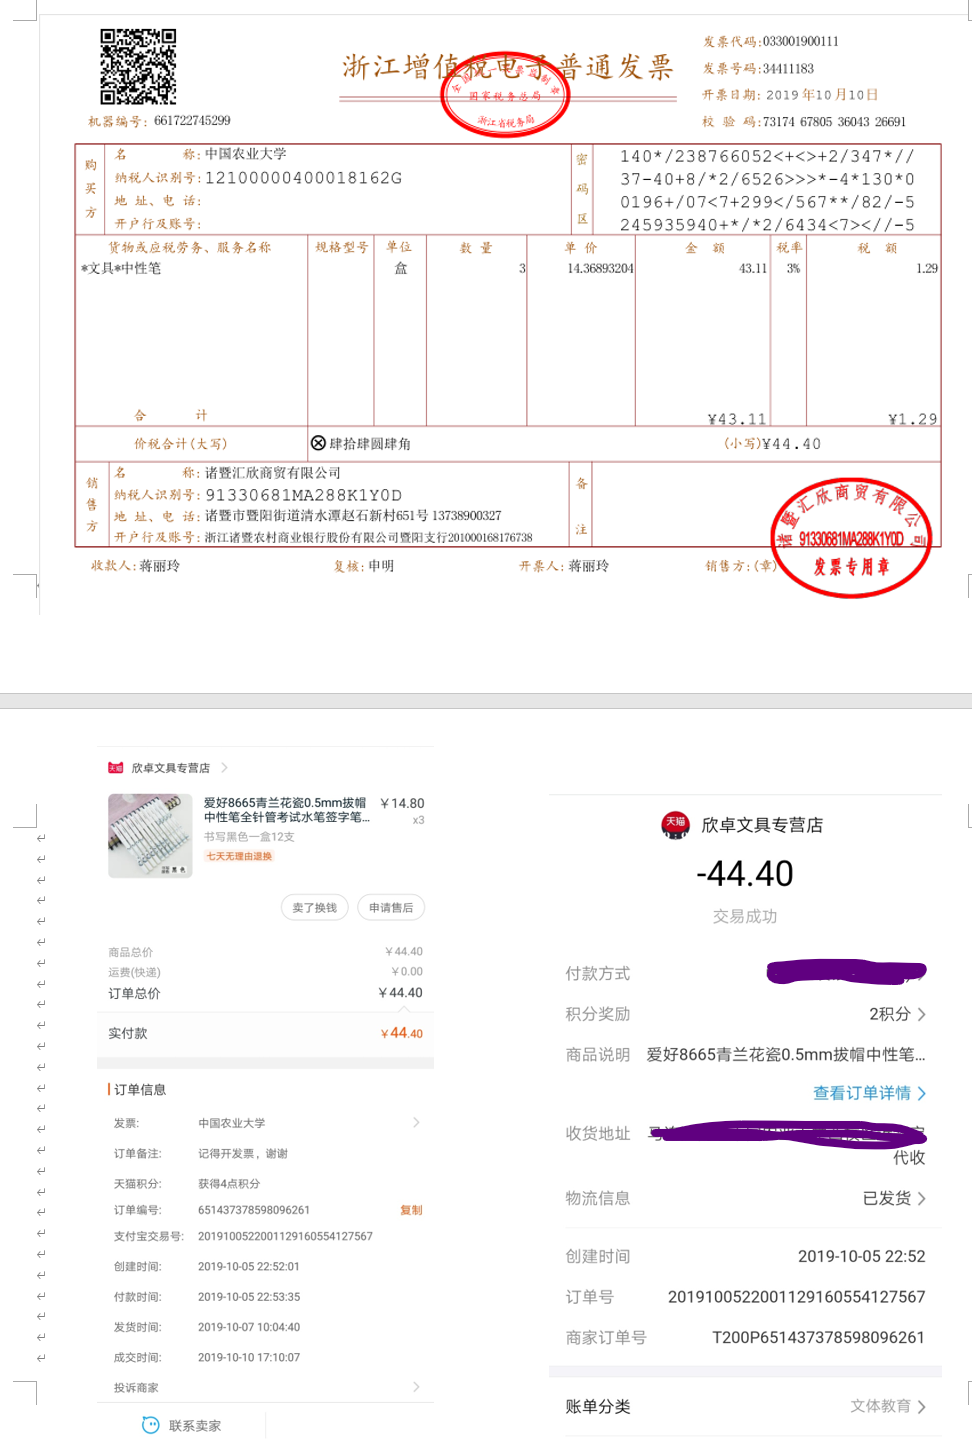
\includegraphics[width=0.8\textwidth]{fig/发票报销.png}
    \caption{支付与订单截图在同一页,发票在一页;两张顺序:先支付与订单截图,再发票
    即,同一商品占据两页}
\end{figure}

\chapter{附录}
\section{路书制作方法}
\label{chapter:路书制作方法}
这里我以行者为例。

1.首先打开行者官网 \href{http://www.imxingzhe.com/}{http://www.imxingzhe.com/}。

        \begin{figure}[H]
            \begin{center}
            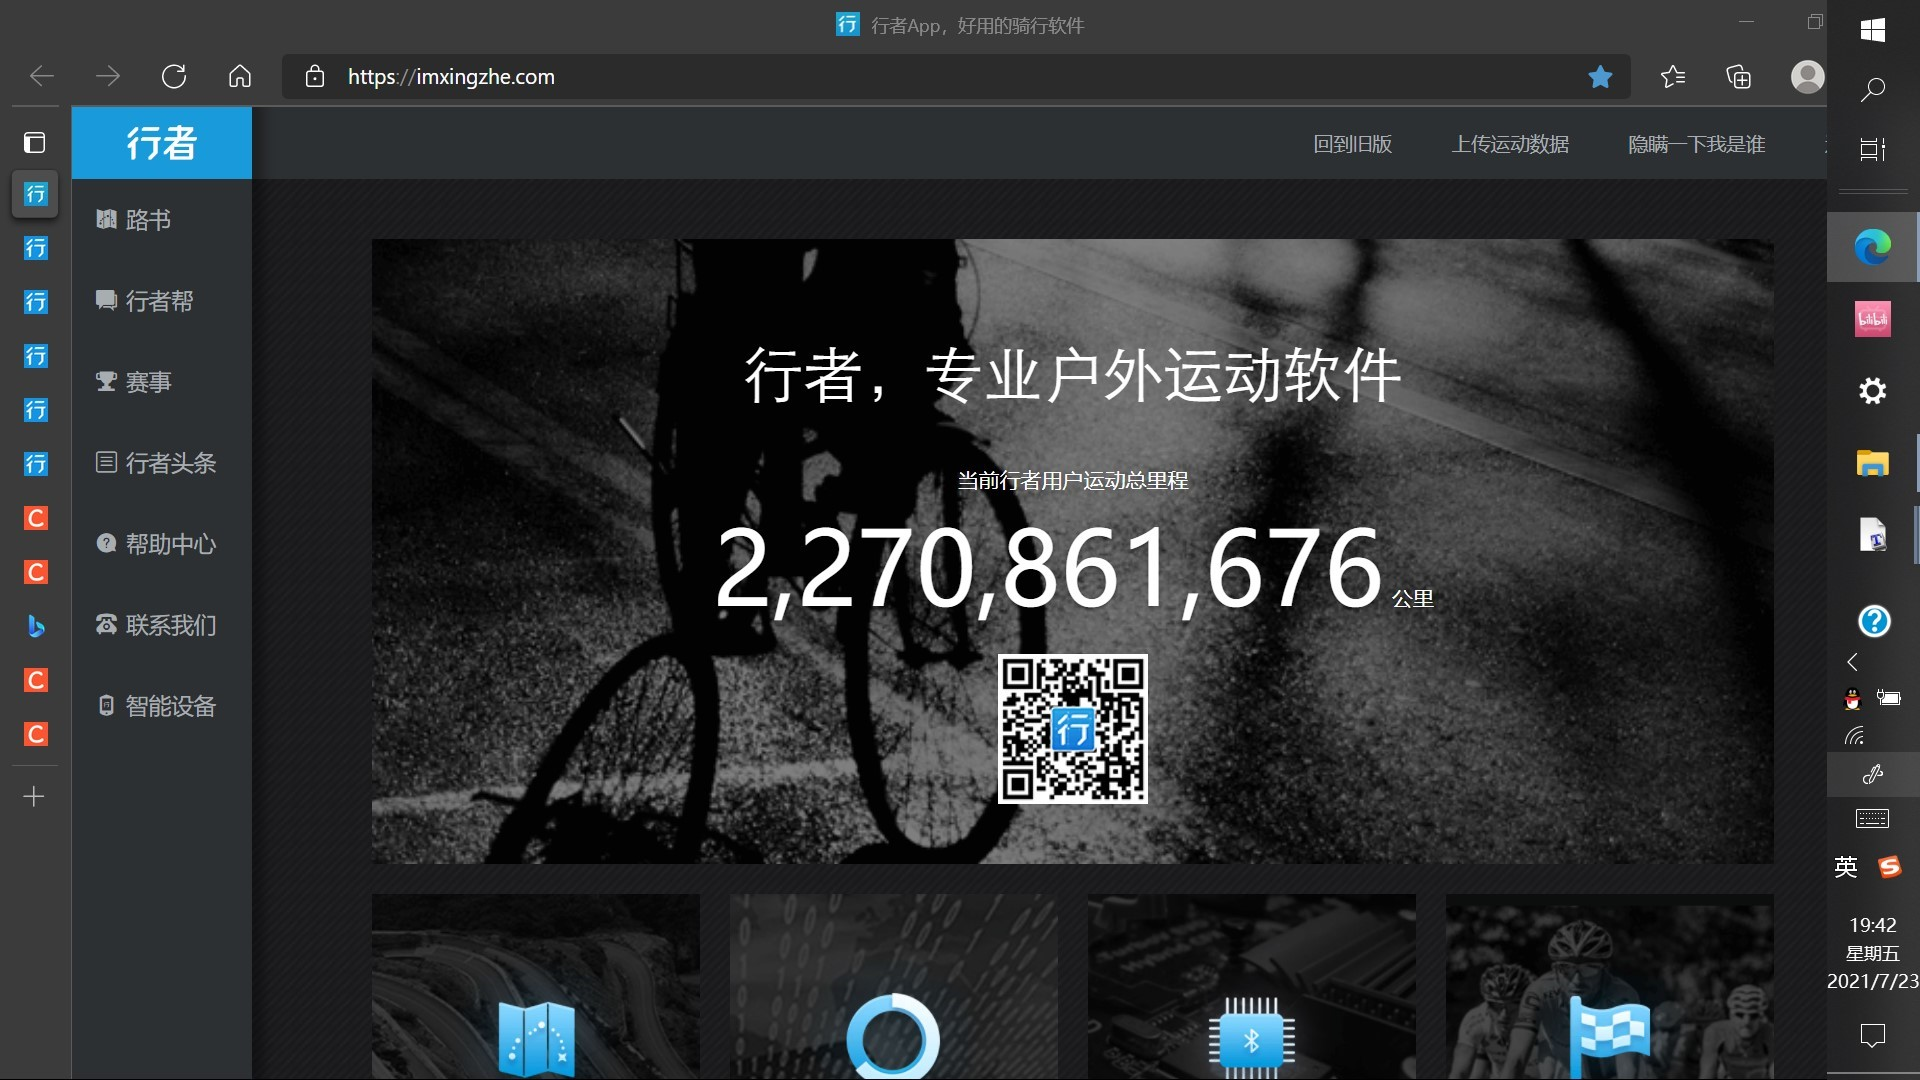
\includegraphics[width=0.6\textwidth]{fig/行者1}
            \end{center}
        \end{figure}

2.点击左侧菜单栏''路书``后点击''制作路书``。
       \begin{figure}[H]
            \begin{center}
            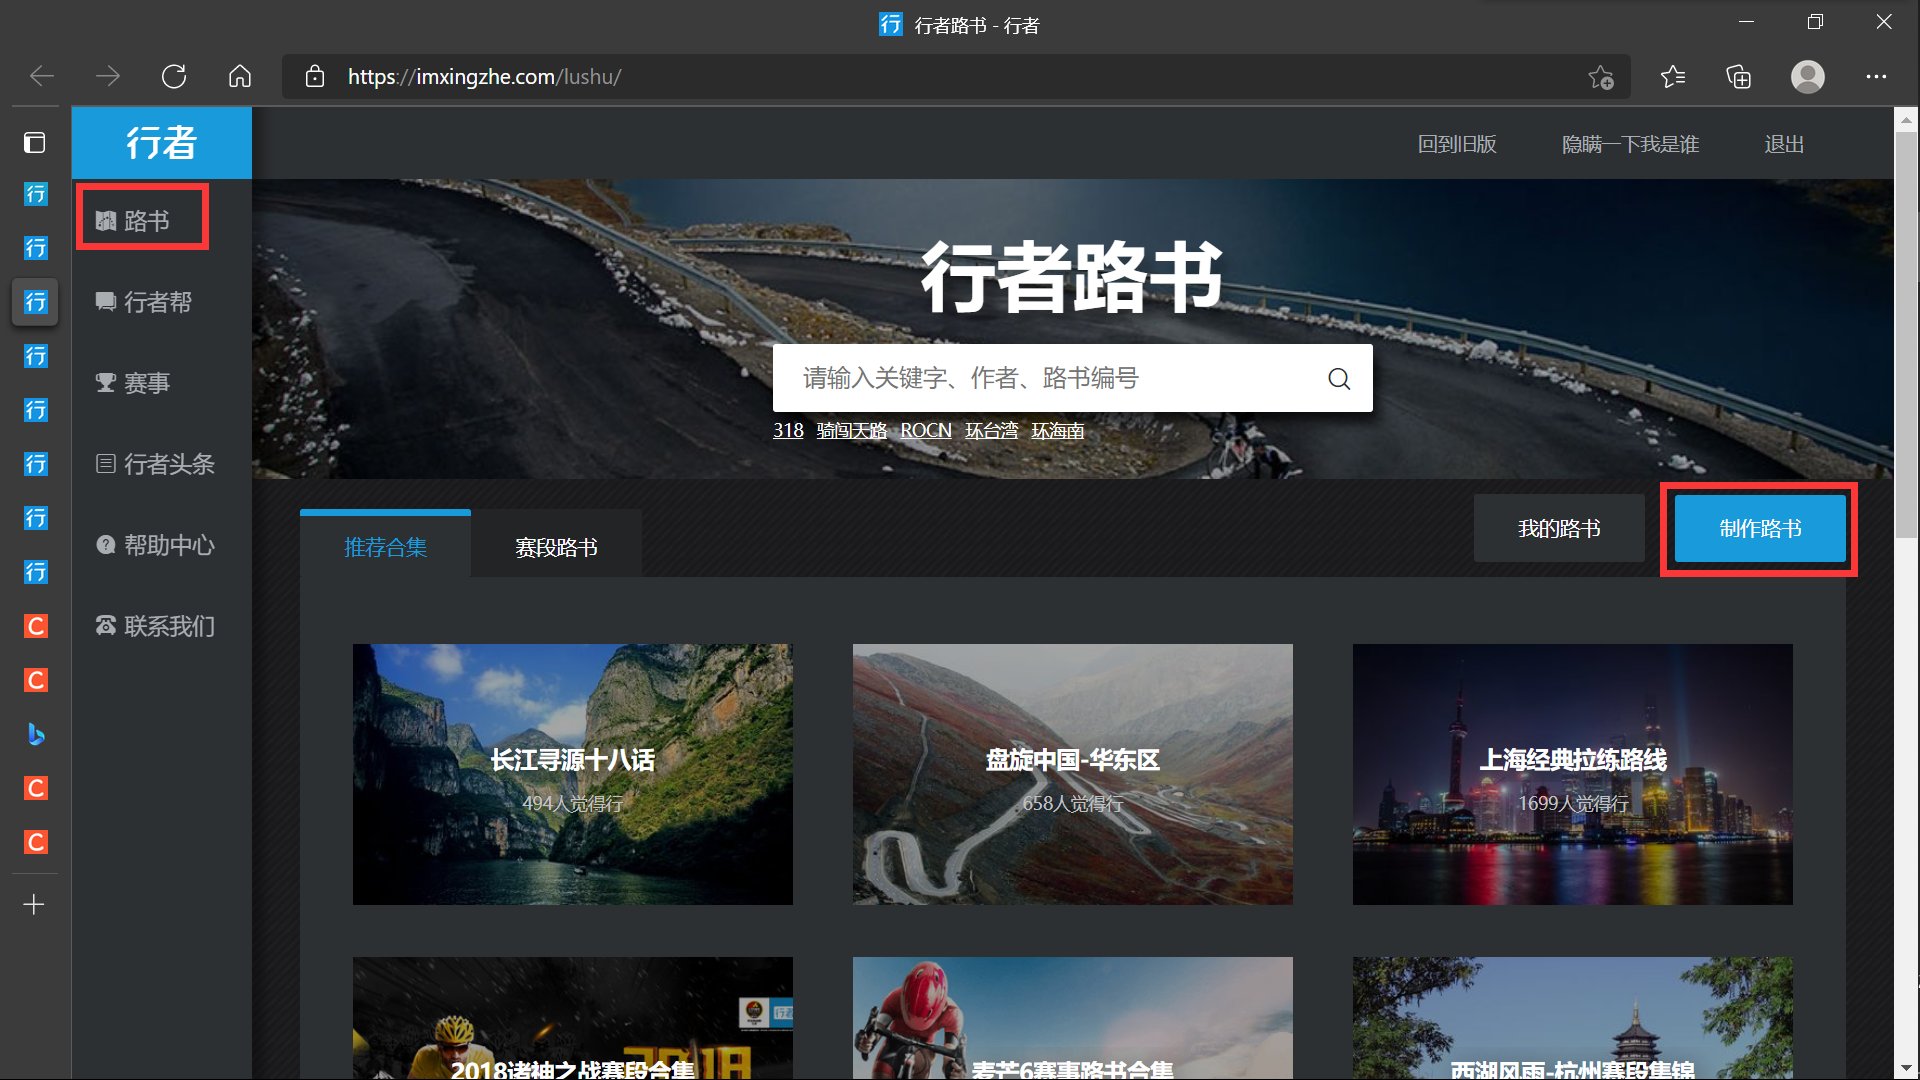
\includegraphics[width=0.6\textwidth]{fig/行者2}
            \end{center}
        \end{figure}

3.选择''百度模式``。
       \begin{figure}[H]
            \begin{center}
            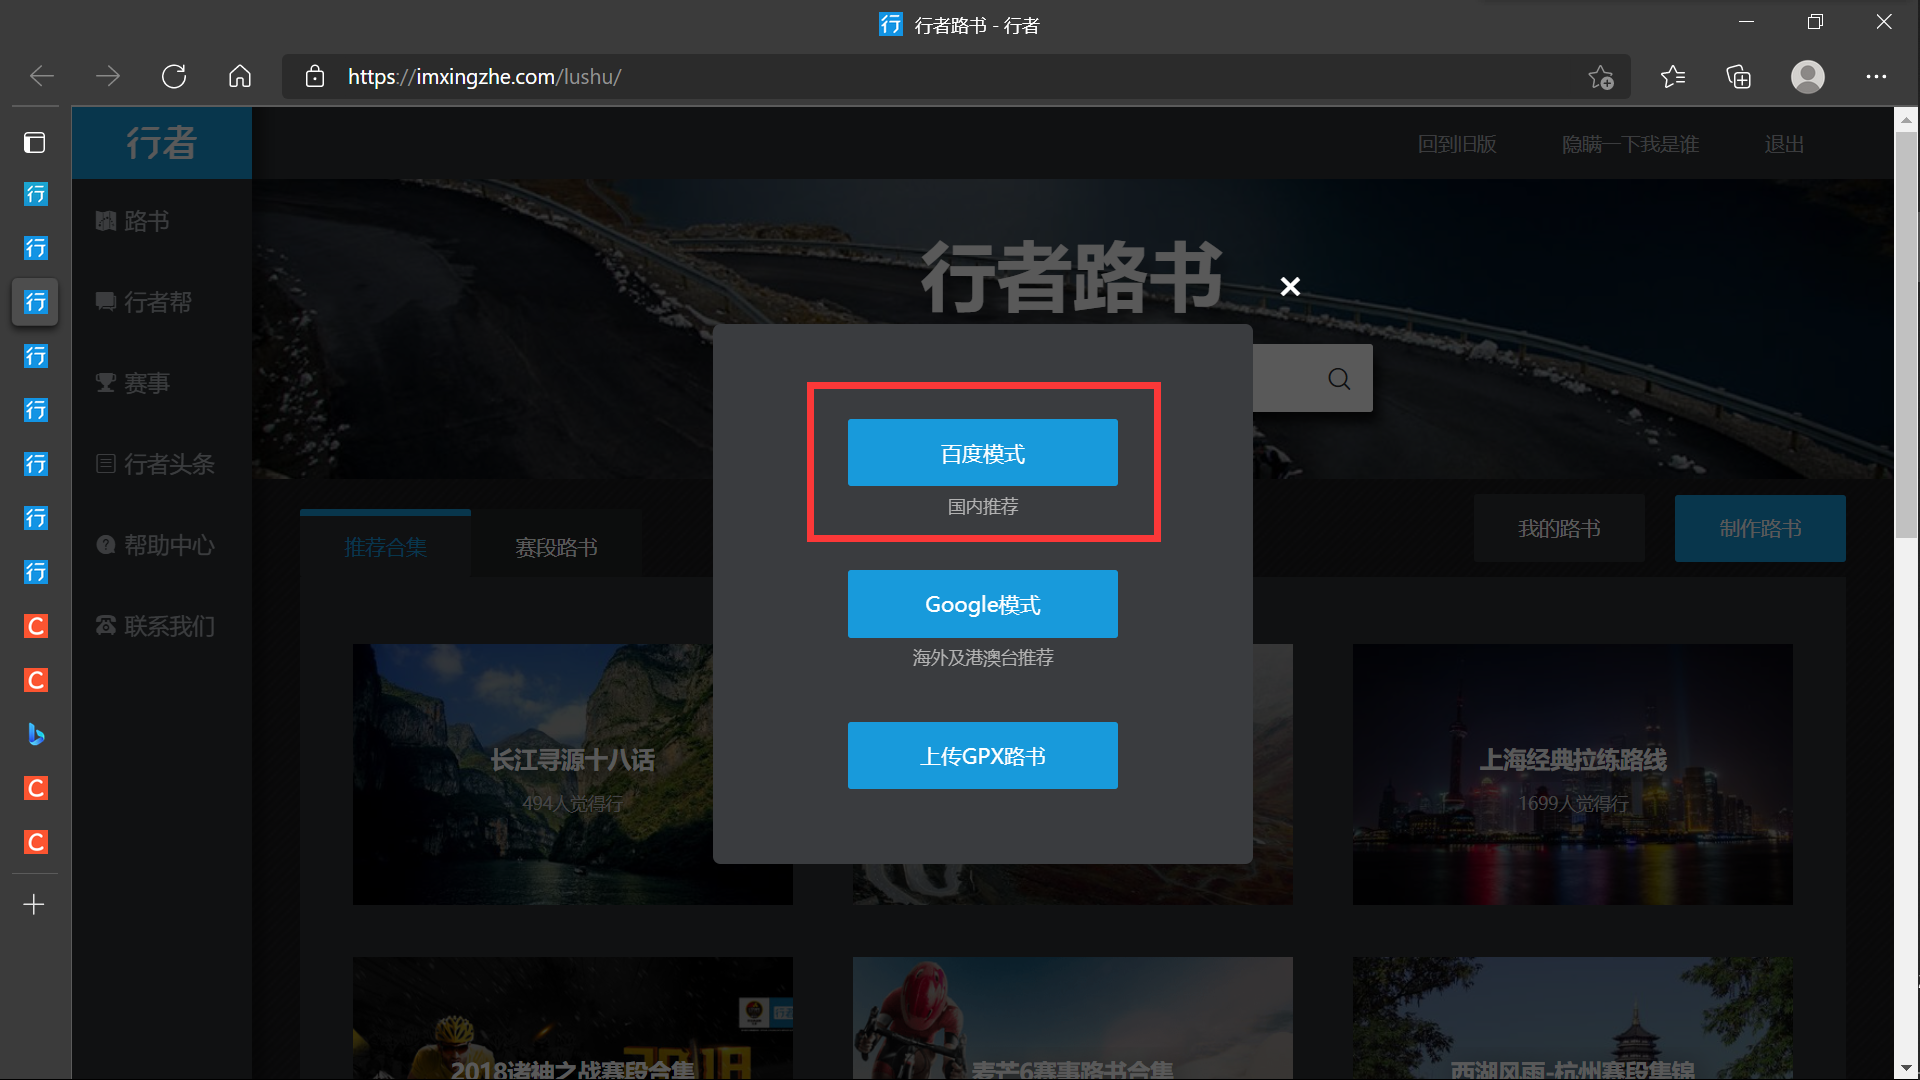
\includegraphics[width=0.6\textwidth]{fig/行者3}
            \end{center}
        \end{figure}

4.在这里可以搜索地名
       \begin{figure}[H]
            \begin{center}
            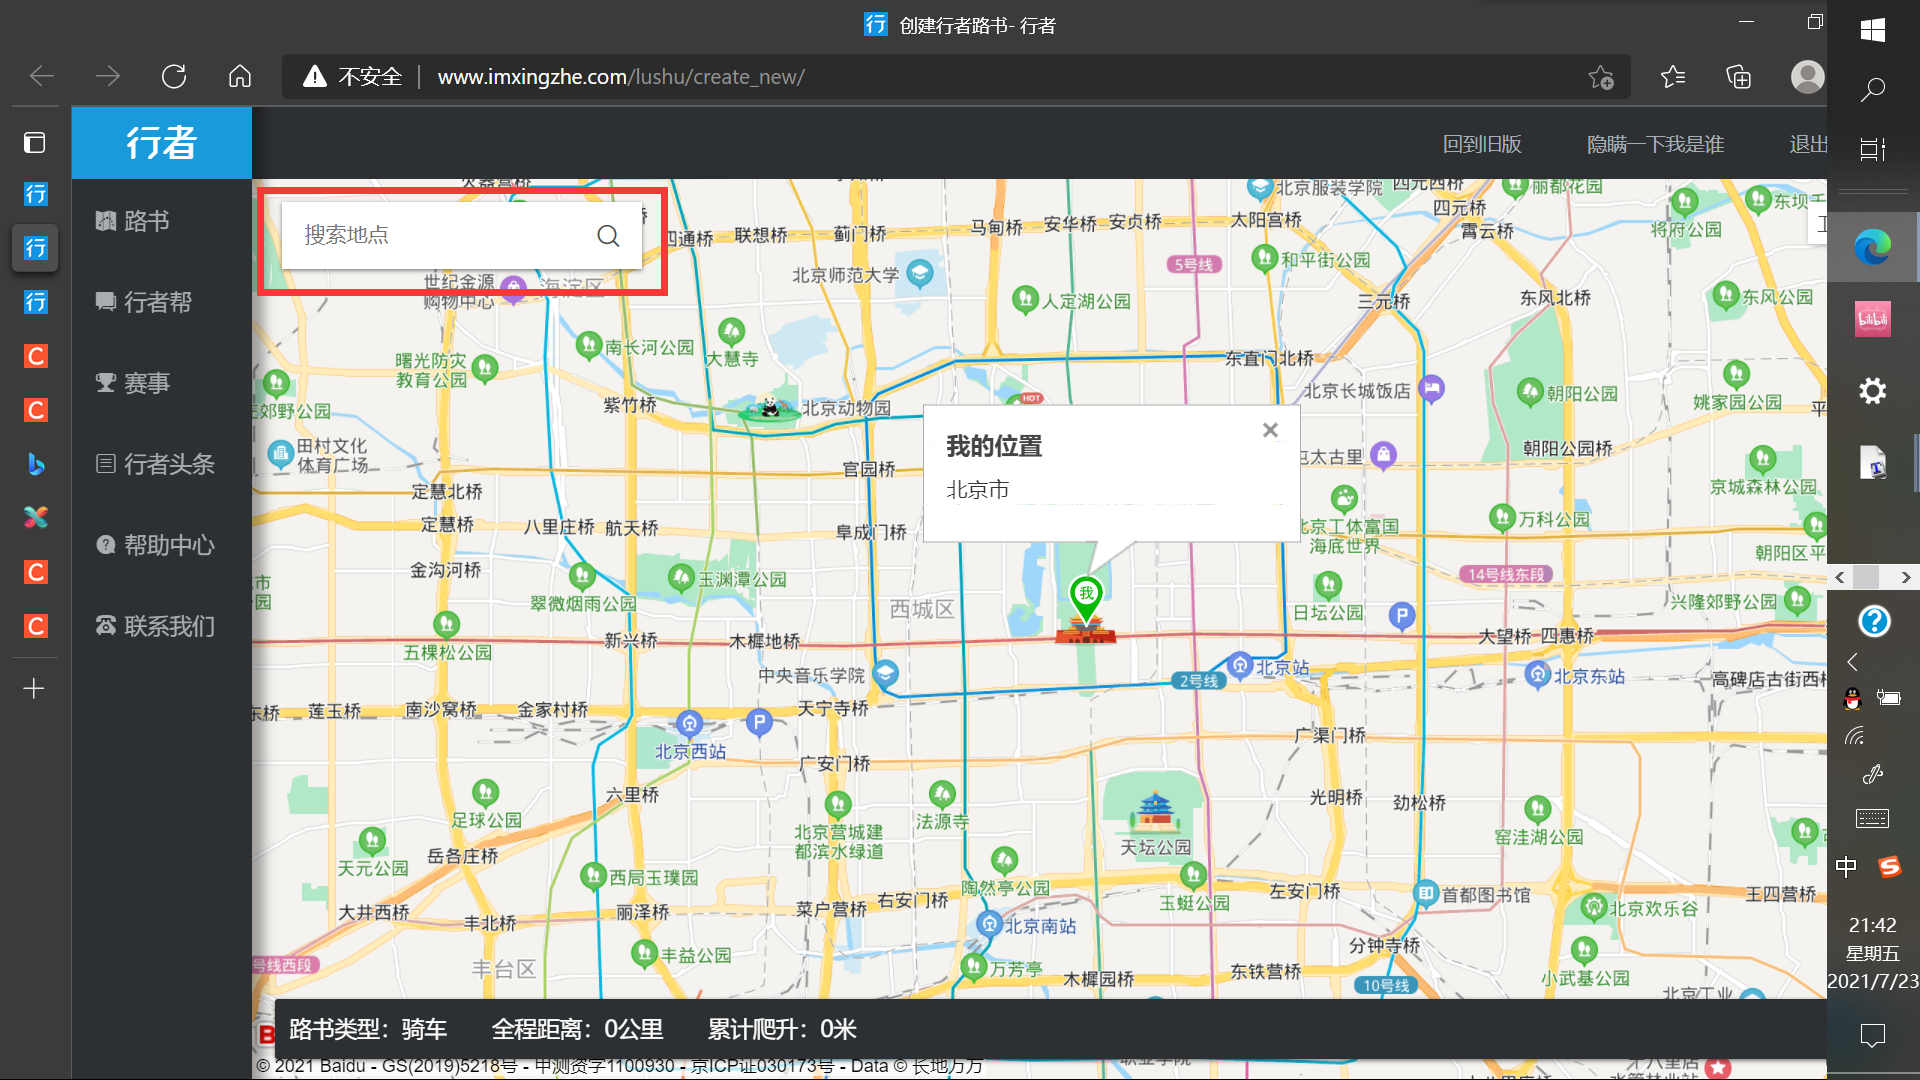
\includegraphics[width=0.6\textwidth]{fig/行者4}
            \end{center}
        \end{figure}

5.以起点为''中国农业大学东校区``,终点为''中国农业大学西校区``为例。
       \begin{figure}[H]
            \begin{center}
            \includegraphics[width=0.6\textwidth]{fig/行者5}
            \end{center}
        \end{figure}

6.选择具体起点位置,右击选择''创建起点``。
       \begin{figure}[H]
            \begin{center}
            \includegraphics[width=0.6\textwidth]{fig/行者6}
            \end{center}
        \end{figure}

7.在预期路线上选择途经点,陌生路线建议探路。途经点生成之后可拖动。
       \begin{figure}[H]
            \begin{center}
            \includegraphics[width=0.6\textwidth]{fig/行者7}
            \end{center}
        \end{figure}

8.在经过一系列创建途经点操作后,形成了一条完整的线路,如图。
       \begin{figure}[H]
            \begin{center}
            \includegraphics[width=0.6\textwidth]{fig/行者8}
            \end{center}
        \end{figure}

注意事项:

1.在道路四通八达(如城区)的时候,自动生成的路线不是理想路线时,可通过设置更多途经点,来纠正成理想路线。

2.设置途经点过多,画面拥挤时,可通过点击已生成的途经点,点击取消''显示途经点``来隐藏。
       \begin{figure}[H]
            \begin{center}
            \includegraphics[width=0.6\textwidth]{fig/行者9}
            \end{center}
        \end{figure}

3.点击已生成的途经点,可以添加备注,手机导航路书时点击途经点可以看到。
       \begin{figure}[H]
            \begin{center}
            \includegraphics[width=0.6\textwidth]{fig/行者10}
            \end{center}
        \end{figure}

4.建议除休息点以外的途经点全部隐藏。

\section{北京高校车协通讯录}
\label{ssec:北京高校车协通讯录}
\begin{table}[H]
    \centering
    \tiny
    \begin{tabular}{|c|c|c|c|c|}
    \hline
        学校 & 协会名称 & 协会成立日期 & 协会官方邮箱 & 协会微信公众平台 \\ \hline
        华北科技学院 & 华科车协 & 2003/3/28 & huakechexie@126.com & 华科车协CACS \\ \hline
        北京交通大学 & 交大车协 & 2000/9/1 & 15221277@qq.com & bjtu cycling(交大车协) \\ \hline
        中国政法大学 & 万里自行车协会 & 2001/9/1 & wanlichexie\_cupl@163.com & wanlichexie \\ \hline
        对外经济贸易大学 & 蚂蚁车协 & 2004/4/6 & 465707976@qq.com & 蚂蚁车协公众号 \\ \hline
        北京体育大学 & 北体车协 & 2013/9/24 & bsucycle@163.com & 北体车协 \\ \hline
        北京联合大学 & 自行车协会 & 2016/9/30 & 1289681197@qq.com & BuuCycling \\ \hline
        北京信息科技大学 & BISTU\_CAST单车社 & 2015/9/1 & 1453898960@qq.com & 无 \\ \hline
        北京林业大学 & 悦野车协 & 2004/11/5 & bjfuyueyechexie@163.com & 北林悦野车协 \\ \hline
        中国地质大学(北京) & 中国地质大学游骑兵自行车协会 & 2004/11/5 & cugbcycle@163.com & 中国地质大学自行车协会 \\ \hline
        北京航空航天大学 & 北航行者自行车协会 & 2010/10/7 & xingzhechexie@163.com & 北航行者车协 \\ \hline
        华北电力大学 & 征途车协 & 2007/5/18 & chexie@163.com & 华电征途车协 \\ \hline
        北京物资学院 & 北京物资学院FAR骑行社 & 2011/10/15 & bwufar@163.com & 无 \\ \hline
        北京石油化工学院 & 鹰隼车协 & 2013/4/15 & biptchexie@163.com & BIPT北石化骑行社 \\ \hline
        北京邮电大学世纪学院 & 骑迹车协 & 2014/3/21 & bysjqiji@163.com & 北邮世纪骑迹车协 \\ \hline
        北京印刷学院 & 印迹车协 & 2014/5/23 & bigc\_yinjichexie@163.com & BIGC车协 \\ \hline
        北京工业大学 & 北京工业大学BJUT骑行社 & 2006/4/2 & bjutchexie@foxmail.com & 北工大骑行社 \\ \hline
        北京化工大学 & 追风车协 & 2006/11/9 & buctzhuifeng2014@126.com & BUCT追风车协 \\ \hline
        北京科技大学 & 贝壳车协 & 2001/5/20 & ustb\_bike2001@163.com  & 贝壳自行车协会 \\ \hline
        首都经济贸易大学 & CUEB校车队&车协 & 2017/9/28 & RIDECUEB@163.com & 经贸骑行社 \\ \hline
        首都医科大学 & 首都医科大学自行车爱好者协会 & 2013/9/4 & ccmubike@163.com & CCMU车协小伙伴 \\ \hline
        中国地质大学 & 中国地质大学游骑兵自行车协会 & 2004/11/17 & cugbcycle@163.com & cugbcycle \\ \hline
        中国农业大学 & 阳光自行车协会 & 2001/3/15 & sunnybikefromcau@163.com & 阳光车协 \\ \hline
        防灾科技学院 & 震远自行车协会 & 2013/11/5 & zhenyuanchexie@163.com & zhenyuan3355 \\ \hline
        北京电子科技职业学院 & nexus & 2015/5/8 & 2576940249@qq.com & 无 \\ \hline
        北京吉利大学 & MAX车协 & 2011/10/23 & maxchexie@163.com & 北京吉利大学MAX自行车协会 \\ \hline
        中国人民大学 & 中国人民大学自行车协会 & 2012/4/16 & rucchexie@163.com & cycling\_RUC \\ \hline
        中国石油大学(北京) & 流云车协 & 2004/4/10 & liuyunchexie@126.com & 流云车协 \\ \hline
        中国人民公安大学 & 骑兵车协 & 2012/5/5 & cappsuc@126.com & cappsuc—new \\ \hline
        北京大学 & 北京大学自行车协会 & 1995/10/25 & beidachexie@126.com & capu北大车协 \\ \hline
    \end{tabular}
    \caption{北京高校车协通讯录}
    \label{tab:北京高校车协通讯录}
\end{table}
\clearpage
\section{团队骑行安全协议}
请参与活动人员仔细阅读以下协议内容,并在免责声明处相应位置签字。
\begin{enumerate}[label={\chinese*、}]

\item 队员必须听从队长及主要负责人的工作安排,如有异议协商解决。

\item 队长有权利在活动前以合理理由劝退某些已报名的队员。

\item 队员不得中途退出活动或私自离队;在到达目的地后亦不可擅自离队活动。

\item 严禁未经允许的情况下戏水游泳。

\item 严禁酗酒、吸烟、赌博。

\item 保管好自己的自行车,尤其是借车的队员,请认真爱护车辆并在活动结束后听队长安排清洗护理;如有损坏、丢失的情况,需按原价赔偿。

\item 骑行过程中:
\begin{itemize}
\item 严格遵守交通规则;
\item 严禁队员擅自超越前骑;
\item 行进中严格服从前骑或队长指挥,保持单列或双列队形,禁止三列及三列以上并行。
\item 禁止相互追打、竞速。
\item 下坡时,要保持队形,不得猛冲,不得无故超车;
\item 骑行中队员不得用耳机听mp3等音乐播放设备;
\item 队长有权利阻止队员进行无把握的xc放坡,爬树等行为。
\item 队员在骑行过程中,如果有体力不支或身体不适的情况,要及时向队长或相关负责人反映,队长会根据队员的实际情况及时调整骑行速度和休息时间。
\end{itemize}
\item 队员须在活动中自觉维护个人、协会及学校的形象。
\item 保护环境,禁止乱扔垃圾,乱涂乱画。
\item 队员有权监督队长等活动负责人是否遵守上述规定。
\item 队员须先重视、确保自身安全,在有能力的情况下再帮助他人。
\item 不能让女队员单独离队。
\item 团队中各职务务必遵守职务要求。
\item 注意保持车距适中,速度越快,相邻车辆之间距离应越远。
\item 不允许在队伍中急刹车,车子出问题时应先示意后方队员,再出列减速靠边停。

\item 不戴头盔严禁上路。

\end{enumerate}
\newpage
\thispagestyle{empty}
\begin{center}
\heiti\Huge 免责声明
\end{center}

户外运动本身具有一定危险性和不可预知性,参加者必须均为满18周岁且均被视为具有完全民事行为能力的人,参加者必须对自己的行为以及造成后果负责。活动队长以及有团队职务的成员需接受全体队员的监督,有责任在《团队骑行安全协议》范围内保证队员人身安全;有责任与财务商议控制活动花费并公开账目。除此,甲方不对任何户外活动本身具有的风险以及队员违背《团队骑行安全协议》所造成的任何后果负责。\notes{我也不知道为什么这一页能被搞得这么畸形。。。}

\begin{enumerate}
    \item 队员在认真阅读《团队骑行安全协议》后在下方横线上签字,签字表示完全理解并认可《团队骑行安全协议》以及《免责声明》所述全部内容。
    \item 所有队员应严格遵守协议的要求,若违反上述规定,队长有权作出相应惩罚,一切后果自负。
    \item 本协议在活动出发前统一上交活动队长管理。
    \item 该协议与活动最终解释权归属阳光自行车协会理事会。
\end{enumerate}

\vspace{0.3cm}

请务必认真阅读以上内容后签字。

\vspace{0.3cm}

甲方:\underline{中国农业大学阳光自行车协会}

\vspace{0.3cm}

乙方:\underline{~~~~~~~~~~~~~~~~~~~~} 

\section{学习渠道}
\begin{center}
    \begin{tcolorbox}[title=一些推荐的线上资源,text width = 0.8\linewidth]
        \begin{itemize}
            \item B站:
            \begin{itemize}
                \item 知名菜腿
                \item ClUB100
                \item 吴云飞是三脚超人
                \item DS-Studio 
                \item 计指导
                \item 单车基械匠
                \item 迈金科技
                \item 雪大爷是你大爷
                \item 乐百客Lebycle单车
            \end{itemize}
            \item 微信公众号:
            \begin{itemize}
                \item 单车志
                \item 版主聊车
                \item 北京高校车协联盟
                \item 银锤男SilverHammerMan 
                \item 单车基械匠
                \item Cycling point
                \item FixedGear 2021
                \item 美骑
                \item 57318骑行川藏吧           
            \end{itemize}
            \item 书籍:
            \begin{itemize}
                \item《山地车圣经》
                \item《单车圣经》
            \end{itemize}  
        \end{itemize}
    \end{tcolorbox}
\end{center}

\section{常见问题}
\begin{tcolorbox}[title=为什么禁止情侣上路]
    情侣上路会面临很多问题,例如:

    \begin{itemize}
        \item 如果因为ta犯了错,受到了队长的批评,另一半该怎么办?是看着ta被骂不吱声,还是为了自己的恋爱关系而包庇犯错的ta?
        \item 你是前骑,你的另一半摔车了,你是会留下来陪她还是继续履行前骑的职责?
        \item 大家一起的玩的时候,是否会发生发生情侣两个人玩在一起,不与他人互动的情况?
    \end{itemize}

    另外,学生时代的爱情是脆弱的,但我们的队友情确实坚固的。情侣分手之后,队员聚餐是否还能聚齐?
\end{tcolorbox}
\begin{tcolorbox}[title=为什么要让女生在队列前面]
    这是对女生的保护措施之一。

    前骑后的位置是最舒适的位置,能享受到前骑的破风作用。虽然队伍前方风阻不是最小的,但在后面的话,往往会因为种种原因需要不停的追队伍,相对看来队伍前列更为轻松。而且,前面的位置也更加安全,因为来自前骑的口号一定是最有效,最及时的。
       \begin{figure}[H]
            \begin{center}
            \includegraphics[width=0.6\textwidth]{fig/蹭风队形}
            \end{center}
        \end{figure}
\end{tcolorbox}
\begin{tcolorbox}[title=''人酒坡``是什么]
    ''人`` 指的就是身边的队友

    ''酒`` 指的就是活动结束后的酒局

    ''坡`` 指的就是爬坡

    这就是所谓的车协三宝。
\end{tcolorbox}
\begin{tcolorbox}[title=为什么要发短信]
    确实,在现在这个新时代,发微信发群公告似乎更加方便。但是短信可以让大家感觉到重视。因此,短信是一定要发的。

    发短信的场合有:检车短信(活动报名成功短信)、体测短信、成队短信。
\end{tcolorbox}
\begin{tcolorbox}[title=为什么不能吃饺子/面]

\end{tcolorbox}
\begin{tcolorbox}[title=为什么拉练的过程中不能推车]

\end{tcolorbox}
\begin{tcolorbox}[title=为什么要坐硬座]

\end{tcolorbox}
\begin{tcolorbox}[title=为什么不推荐把手机放在手机支架上导航]
\begin{itemize}
\item 支架与眼睛间的角度、距离问题,导致手机导航在晴天下容易看不清
\item 极度费电
\item 对手机伤害大(暴晒,雨)
\end{itemize}

\end{tcolorbox}
\begin{tcolorbox}[title=为什么下坡的时候要把档位调大]
    众所周知,下坡的时候速度比较快,如果不换大裆,很容易发生踏空的现象。而一旦下坡的过程中,前方出现了意外情况,需要加速,或者可能只是慌乱中踩了一下踏板,一旦踏空,都会使驾驶者心理更加恐慌,从而发生意外。
\end{tcolorbox}
\begin{tcolorbox}[title=驮包与旗杆不相容?]
非也非也,只要把旗杆固定在后上叉和货架上就可以让旗杆远离车座,所以放弃后下叉吧。还有,旗杆绑车左侧。
       \begin{figure}[H]
            \begin{center} 
            \includegraphics[width=0.3\textwidth]{fig/驮包和大旗}
            \end{center}
        \end{figure}
\end{tcolorbox}
\begin{tcolorbox}[title=怎样背驮包]
如果我们用手提着驮包,它不仅会妨碍我们走路,还会占用一只手。
        \begin{figure}[H]
            \begin{center}
            \includegraphics[width=0.2\textwidth]{fig/菁宏驮包}
            \end{center}
        \end{figure}
一前一后地把驮包扛在肩上会感觉轻很多,还不占手。
        \begin{figure}[H]
            \begin{center}
            \includegraphics[width=0.2\textwidth]{fig/王上林驮包}
            \end{center}
        \end{figure}
放在头上也不是不行。       
        \begin{figure}[H]
            \begin{center}
            \includegraphics[width=0.2\textwidth]{fig/林琛宇驮包}
            \end{center}
        \end{figure}
\end{tcolorbox}
\begin{tcolorbox}[title=这份手册为什么要用 \LaTeX 来写,\LaTeX 相比于 word 有什么好处]
    \begin{itemize}
        \item  控制感。凡是刚刚学会了 \LaTeX 的会有种感觉,就是其他的工具不想用了,\LaTeX 输出质量和控制感,令人非常愉悦,比如一个命令,可以让整体的格式变化,一个命令可以产生非常棒的输出效果。自己改改东西,整体会变成非常自己喜欢的样子,令人心旷神怡。
        \item  便于传输和多人协同编译。众所周知,在一个人的电脑上写好的 word 文档,在另一个人那里可能格式完全不一样了。而 Tex 文件作为一个文本文件,不会在传输的过程中发生格式的变换。同样的,一份写的很好的 word 文件,在被另一个 word 使用者改写后,很容易发生格式失控的情况,并且其他的人很难知道他究竟动了哪里造成了这样的情况。
    \end{itemize}

\end{tcolorbox}
\begin{tcolorbox}[title=为什么车协总是有这么多nt规定,比如不允许擅自超越前骑或者指责前骑]
    如果一个规定,被写成大字,贴在你一眼就能看到的地方。

    那么,很有可能,上面的内容是由鲜血换来的教训。
    
    比如,进工地要带安全帽。
    
    水泥墙面不应该掉砖头,否则就是墙面有问题。
    
    但你不应该用自己的脑袋赌它没问题。
\end{tcolorbox}
\section{值得被记住的话} 
\begin{itemize}
    \item 车是载体,情最动人
    \item 铁打的车协,流水的阳光
    \item 做执委最重要的是自己先玩好
    \item 我说车协千万好,不如一次秦皇岛
    \item 一个人可以骑得更快,一群人可以骑的更远
\end{itemize}
\section{注释}
\listoftodos[Notes]
\section{短信/通知模板}
\label{ssec:晚训通知}
\begin{center}
    \begin{tcolorbox}[title=晚训通知,text width = 0.8\linewidth]
        @ 全体成员 \#晚训通知\#
    
        东区负责人:XXX
        
        西区负责人:XXX
        
        集合时间签到时间:n:nn-n:nn
        
        集合地点:
        
        东区:操场西南角
        
        西区:操场沙坑处
        
        晚训内容:2圈热身+N圈慢跑(变速跑)+1圈冲刺跑,外加俯卧撑等一系列上肢锻炼
    
        \end{tcolorbox}
    \end{center}

\label{subsec:检车通知}
\begin{center}

    \begin{tcolorbox}[title=检车通知,text width = 0.8\linewidth]
        
    亲爱的阳光: 
    
        恭喜你成功报名xxx活动,此消息来自本次活动队长xxx和xxx。现通知有关xx日(周x)检车的相关事宜,务必仔细阅读以下内容:
              
        【检车流程】签到→领取安全协议→队长发言→有车的开始检车/没车的由实践部带去车棚取车→检车→试骑→借车的归还至车棚/解散
              
        【时间】xx日(周x)中午12:30
              
        【地点】东区:奥运场馆西侧雕像旁\par 西区:7号楼和8号楼之间的空地处
              
        【注意】 请检车人员带好手机
              
        【检车要求】必须本人到现场,原则上不允许请假,若实在无法参加,请于今晚23点59分前联系我,说明原因。迟到且未提前请假者,需视情况处罚跑圈/检讨,严重者取消活动资格!
              
        再次强调时间,请勿迟到,请勿迟到,请勿迟到!!!
              
        收到请于今日23:59前回复``xx收到'',例:张三应回复``张三收到''
    \end{tcolorbox}
    \end{center}

\begin{center}
    \begin{tcolorbox}[title=新生见面会短信,text width = 0.8\linewidth]
    \end{tcolorbox}
\end{center}

\begin{center}
    \begin{tcolorbox}[title=体测通知,text width = 0.8\linewidth]
    \end{tcolorbox}
\end{center}

\begin{center}
    \begin{tcolorbox}[title=成队通知,text width = 0.8\linewidth]
    \end{tcolorbox}
\end{center}
\begin{center}
\begin{tcolorbox}[title=暑期跑步体测短信模板]
    
    阳光车协20xx暑期预备队员,你好:
    
    经过x周的晚训和拉练,通过努力,你已获得的积分满足暑期选拔方案中的体测要求,直接获取到参加阳光车协20xx年暑期远征选拔体测资格,现正式通知你:跑步体测时间为本周X(x月xx日)xx:xx,地点在车协东区晚训处;妙峰山骑车体测时间为下周X(x月x日),详细情况请关注公众号及相关通知。
    
    请于今晚xx:00前回复''收到+姓名``。
    
    祝取得满意体测成绩,体测,加油!
    
    阳光车协理事会
    \end{tcolorbox}
\end{center}
\begin{center}
    \begin{tcolorbox}
    
        跑步体测
        
        【签到时间】
        
        志愿者:18:00-18:10
        
        暑期预备队员:18:20-18:30
        
        【签到地点】
        
        东区操场西南角
        
        【流程】
        
        签到→发放号码布→男生热身(两圈慢跑+准备活动)→男生开跑→男生结束→男生拉伸/女生热身→女生开跑→女生结束→女生拉伸→吃瓜
        
        【注意事项】
        
        1. 体测前有课的小阳光,准备一些吃的在四点左右吃掉,保证能量充足
        
        2. 带一件长袖,跑完注意保暖
        
        加油!
        \end{tcolorbox} 
\end{center}

\section{头盔清洁}
\label{sec:头盔清洁}
\begin{itemize}

\item 清洗外壳

直接清洗剂+常温水,泡+刷。
\begin{figure}[ht]
\centering
\includegraphics[width=7cm]{fig/头盔清洁1}
\hspace{10pt}  %2张图片的水平距离
\includegraphics[width=7cm]{fig/头盔清洁2}
\end{figure}

\item 清洗扣带

扣带是接触脸的东西,吸收汗水,特别脏,所以要来一剂猛的,多点洗剂,刷干净了。

\begin{figure}[H]
    \begin{center}
    \includegraphics[width=0.4\textwidth]{fig/头盔清洁3}
    \end{center}
\end{figure}

\item 清洗内衬

内衬取下,手洗即可。
\begin{figure}[H]
    \begin{center}
    \includegraphics[width=0.4\textwidth]{fig/头盔清洁4}
    \end{center}
\end{figure}

\item 干燥
 
通风阴凉处晾干,不要用吹风机长时间吹泡沫部分。

\end{itemize}

简单清洁只须清洗扣带、内衬,擦拭外表面。

%\chapter{车协物品}
%\section{宣传用品}
%\section{骑行用品}
%\section{修车物品}
%\begin{itemize}
%    \item 组合
    
%    顶尖品牌:PARK\ TOOL 有点小贵

%    质量差的组合会把螺丝拧滑丝,车协可以买一个质量好一点的组合比如PARK TOOL 。
    
%    如果是自用的话,可以买便宜一点的。

%    推荐产品:淘宝搜索洛克运动户外专营店,在店铺里搜索''补胎``,一套家伙才19.8,便宜好用
%    \begin{figure}[H]
%        \begin{center}
%        \includegraphics[scale=0.3]{洛克兄弟_补胎工具.png}
%        \end{center}
%    \end{figure}
%\end{itemize}
\chapter{后记}
\section{第一版后记}
又是一年秦皇岛。

满打满算,这本手册已经写了一年了吧。这一年来,我在这上面花了很大的辛苦,一点一点地修改手册结构,格式,内容。就像是看着孩子的成长一样,我看着它一点一点变得更好,真的很开心。

在2021年换届的时候,我把它打印了十份,给了下一届执委,得到了广泛的好评。

在今年实践队的社会实践的过程中,我把接下来一年的手册维护任务交给了王上林,看起来她很靠谱的样子。

总感觉自己有很多话想说,可真的坐在电脑前,我却不知道该说些什么了。

就这样吧。
\hfill 张\hspace{3mm}阳 \hspace{10mm}

\hfill 2021年秋,农大\hspace{2mm}
\end{document}